% Template for BSc final reports
% CAE Department - Istanbul Technical University
%
% INSTRUCTIONS
% (1) Compile using LuaLatex (it is the successor of pdflatex). To check this on Overleaf, click on the Menu on the top left.
% (2) Complete the SETUP below
% (3) Students of Istanbul Technical University can claim a free premium Overleaf account, please check
% Claim the free premium account because as your report becomes more and more complex, you may reach the timeout limit of the free account.
% Alternatively you may setup LateX compiler in your machine and use GitHub or similar environments for teamwork.

%%%%%%%%%%%%%%%%%%%%%%%%%%%%%%%%%%%%%%%
% DO NOT MODIFY FROM HERE ...
\documentclass[10pt]{itu_cae_dissertation}

\usepackage[style=ieee,backend=biber,hyperref=auto]{biblatex}
\addbibresource{references.bib}



% ... TO HERE
%%%%%%%%%%%%%%%%%%%%%%%%%%%%%%%%%%%%%%%


%%%%%%%%%%%%%%%% SETUP %%%%%%%%%%%%%%%%
%%%%%%%%%%%%%%%%%%%%%%%%%%%%%%%%%%%%%%%
% EDIT THE FOLLOWING INFORMATION WITH YOUR DATA
% IF YOU ARE DOING AN MSC IGNORE PART B
% LINES STARTING WITH % ARE COMMENTS. UNCOMMENT JUST ONE OF A SET OF OPTIONS
% MAKE SURE YOU CHECK AND UPDATE ALL INFORMATION, INCLUDING SUBMITYEAR


%%%%%%%%%%% PART A %%%%%%%%%%%
% PICK A DEGREE FROM THE LIST BELOW 
% BY COMMENTING OUT/IN YOUR DEGREE
% DO NOT MODIFY THE NAMES
%\degree{MEng}
\degree{BEng}
%\degree{MSc}

\title{Modbus Based Smart Energy Tracking and Control and System}
\subtitle{} % use \subtitle{} to remove the subtitle
\lecture{KON 4902 Control $\&$ Automation Engineering Design II}
\author{Kürşat Döşkaya \\ Kenan Selçuk \\ Burak Uğur}
\sid{040200512, 040200509, 040170140} % Fill your student ID to here
\supervisor{Dr. Onur Akbatı} 
\submityear{2025}



% PICK A COURSE FROM THE LIST BELOW 
% DO NOT MODIFY THE NAMES
\course{Control $\&$ Automation Engineering}
%\course{Robotics $\&$ Autonomous Systems Engineering}



% Do you want a list of figures?
% Do you want a list of tables?
% Do you want an acknowledgement page?
% Do you want a list of acronyms?
\setboolean{list_of_figures}{true} % false or true - Default is true
\setboolean{list_of_tables}{true} % false or true - Default is false
\setboolean{acknowledgement}{false} % false or true - Default is true
\setboolean{acronyms}{true} % false or true - Default is true
\setboolean{symbols}{true} % false or true - Default is true

% If you want to print your thesis, consider changing the command below to true. If true, the command adds labels at the edge of the pages which will make easy to identify a chapter running through the pages with the finger. It is just a visual setting. The default values are different for MENG/BEng and MSc as a consequence of the different approval process. In any case, you can change this to either true or false as you prefer.

\setboolean{edge_labels}{true} % default is true 

%The preferred spacing for FYP/MSc reports is doublespacing. This is because it is easier for markers to annotate the document while marking. Some students require the implementation of the singlespacing option. This can be activated below by changing from true to false, but discuss this with your supervisor first.
\setboolean{double_spacing}{true} %Default is true. If you want to change this, ask your supervisor if they are OK with singlespacing.

%%%%%%%%%%% PART B %%%%%%%%%%% 
% Is this an interim report or final report?
\setboolean{final_thesis}{true} % true for final Thesis / false for interim report
%\secondmarker{Second Marker\\[2mm]{\large \textsc Dr Jane Doe}} %If you do not know who your second marker is, use \secondmarker{}

%%%%%%%%%%%%% END SETUP %%%%%%%%%%%%%%%
%%%%%%%%%%%%%%%%%%%%%%%%%%%%%%%%%%%%%%%


% ADDITIONAL PACKAGES
% You can add your packages below. Note that the following packages are already loaded: pgfcore, geometry, bookmark, graphicx, setspace, kantlipsum, fontspec, polygrossia (default English), minitoc, silence, background, xpatch, tikzpagenodes, totcount, fancyhdr, titlesec and the tikz libraries calc, shapes.symbols and shapes.misc  

%Examples
\usepackage{amsmath}
\usepackage{amsfonts}
\usepackage{siunitx}
\usepackage{listings}
\usepackage{algorithm}
\usepackage{algpseudocode}
\usepackage{tikz}
\usetikzlibrary{shapes.geometric, arrows}
\usepackage{adjustbox}
\usepackage{geometry}
\geometry{a4paper, margin=1in}
\usepackage{enumitem}
\usepackage{hyperref}
\usepackage{fontspec}
\usepackage{titlesec}
\usepackage{float}


%...

% ADDITIONAL COMMANDS
%Examples
\DeclareMathOperator{\diag}{diag}
\DeclareMathOperator{\vect}{vec}
%...


\begin{document}

\preamble % Do not change - required

% EDIT THE CONTENT OF THE FILES
% Abstract.tex
% OrigSta_Copyright.tex
% Acknowledgement.tex
% You can find them under the folder 
% "chapters" on the left column

% ADD AS MANY CHAPTERS AS NEEDED
% BY CREATING .TEX FILES IN THE FOLDER chapters
% AND ADDING \input{namechapter.tex} BELOW
\doublespacing % Do not change - required

\chapter{Introduction}
\label{ch1}

%%%%%%%%%%%%%%%%%%%%%%%%%%%%%%%%%%%%%%%
% IMPORTANT
\begin{spacing}{1} %THESE FOUR
\minitoc % LINES MUST APPEAR IN
\end{spacing} % EVERY
\thesisspacing % CHAPTER
% COPY THEM IN ANY NEW CHAPTER
%%%%%%%%%%%%%%%%%%%%%%%%%%%%%%%%%%%%%%%

\section{Motivation}

\begin{itemize}
    \item \textbf{Background and Context:}
    The increasing demand for energy efficiency, sustainability and cost optimization in industry has increased the interest in smart energy management solutions. One of the basic building blocks of these systems is the real-time collection of process data using communication protocols such as Modbus. Programmable Logic Controllers (PLCs) provide a reliable infrastructure for processing this data and implementing control algorithms. In this context, monitoring and optimizing energy consumption is of critical importance not only in reducing operational costs but also in contributing to environmental sustainability goals. This project aims to develop an innovative solution in the field of energy management by combining real-time data analysis and control algorithms.
    \item \textbf{Problem Identification:}
    Despite advances in automation, many industrial systems still face high operational costs and unnecessary environmental impacts due to inefficient energy use. Traditional energy management systems lack real-time data collection and advanced control mechanisms. This makes it difficult to detect abnormalities in energy consumption and to effectively execute optimization processes. Therefore, there is a need to develop intelligent systems that can perform real-time data analysis and optimize energy use using control algorithms such as PID, supported by Modbus-based communication. This project aims to provide a solution to the problem of inefficient energy management by developing an intelligent energy monitoring and control system using control algorithms. .
    \item \textbf{Significance of the Project:}
     This project integrates PLC infrastructure, communication protocols and real-time data analysis by developing a Modbus-based smart energy monitoring and control system. The aim is to optimize energy consumption, increase system stability and reduce operational costs by using real-time monitoring and control algorithms together. The solution developed in the study d offers a scalable structure that can be easily adapted to different industrial applications. Thus, it is aimed to make a significant contribution to energy efficiency and environmental sustainability goals.
    \item \textbf{Personal and Academic Motivation:}
    This study is directly compatible with our academic background in Control and Automation Engineering, combining theoretical knowledge with real-time monitoring, control algorithms and simulation-based system design. Through this project, we aim to develop our competencies in industrial communication, PLC programming, Modbus protocol usage and energy management. We also aim to create a strong infrastructure for our future career plans by contributing to global goals in the field of energy efficiency and sustainability.
\end{itemize}

\section{Design Criteria}
\begin{itemize}
    \item \textbf{Performance Requirements}
    \begin{itemize}
        \item The system must operate with accuracy to optimize energy consumption by at least 10.
        \item Real-time data monitoring time should be provided with a maximum delay of 1 second.
        \item The system must operate with over 95 stability and 98 fault tolerance.
    \end{itemize}

    \item \textbf{Technical Specifications}
    \begin{itemize}
        \item Hardware and software to be used: Siemens S7-1200 PLCSim, Modbus communication,MATLAB.
        \item Modbus
    \end{itemize}

    \item \textbf{Feasibility and Constraints}
    \begin{itemize}
        \item If implemented, the total system cost will be kept at a reasonable level.
        \item Power consumption will be minimized; data acquisition and control units will support low power modes.
        \item Hardware and software integration will be easy, making maintenance and expansion of the system practical.
    \end{itemize}

    \item \textbf{Scalability and Flexibility}
    \begin{itemize}
        \item The system will be modular and will allow for the integration of more sensors or different control algorithms in the future.
        \item It will be designed with flexibility to adapt to different production facilities and virtual factory environments.
    \end{itemize}

    \item \textbf{Safety and Reliability}
    \begin{itemize}
        \item Security measures (password protection, user authorization) will be applied to PLC communication.
        \item The system will be configured to switch itself to safe mode in case of communication interruptions.
        \item Hardware components will be tested periodically to ensure reliability.es
    \end{itemize}

    \item \textbf{Usability and Human Interaction}
    \begin{itemize}
        \item User-friendly monitoring and data analysis interfaces will be developed for operators.
        \item Easy and fast access to energy consumption and system status information will be provided.
    \end{itemize}

    \item \textbf{Environmental and Sustainability Considerations}
    \begin{itemize}
        \item Solutions that will increase energy efficiency will be preferred and carbon footprint will be minimized.
        \item If implemented, care will be taken to select recyclable materials in the components used.
    \end{itemize}
\end{itemize}
\section{Literature Review}
\begin{itemize}
\item \textbf{Previous Work:}
In the first examples of energy monitoring and control systems, manual data collection methods and local control systems were used. With the development of industrial automation, data transmission with Programmable Logic Controllers (PLCs) and Modbus protocol became widespread. Developed by Modicon in 1979, Modbus protocol has gained an important place in energy management applications by providing standard and reliable communication between different devices. Modbus RTU and TCP/IP based solutions have rapidly become widespread, especially for real-time monitoring of energy consumption and data transfer in factories.
\item \textbf{Related Studies:}
In recent studies, energy monitoring and control solutions developed with Modbus-based PLC systems are frequently used. For example, in the Sönmez study, applications were developed for monitoring and managing energy data with Modbus-supported automation systems. In the study conducted by Çetin, it was shown that energy efficiency could be increased by using control algorithms such as PID in motor systems. In addition, the ISO 50001 standard contributes to the continuous improvement-oriented structure of energy management systems.
\item \textbf{Research Gap}
When the existing studies are examined, it is seen that they mostly focus on monitoring energy data, and energy optimization applications with real-time control algorithms are limited. Although many systems perform the task of data collection, advanced control techniques for dynamic energy optimization are not integrated. This project aims to fill this gap by not only monitoring energy consumption, but also optimizing it by analyzing it in real time.
\end{itemize}

\section{Contribution of the Study}
\begin{itemize}
    \item \textbf{Scientific Contributions}
    \begin{itemize}
        \item A smart energy monitoring and control system integrated with Modbus communication has been designed.
        \item A PID-based control approach has been selected for real-time data collection and energy optimization.
        \item The developed system has been tested with comprehensive simulation studies based on Simulink.
    \end{itemize}

    \item \textbf{Technical Contributions}
    \begin{itemize}
        \item A real-time data acquisition and control platform was attempted to be created using Siemens S7-1200 PLCSim.
        \item A reliable communication infrastructure was attempted to be developed using TIA Portal software and Modbus protocol.
        \item System performance; accuracy, data transmission speed and stability were examined in terms of the system.
    \end{itemize}

    \item \textbf{Practical and Industrial Contributions}
    \begin{itemize}
        \item An attempt has been made to develop a system that can be applied in a virtual environment for industrial energy management.
        \item The system architecture has been designed to be easily adapted to a similar system in reality.   
        \item The developed solution serves the purpose of reducing energy costs and supporting sustainable production processes.
    \end{itemize}

    \item \textbf{Academic and Educational Contributions}
    \begin{itemize}
        \item A simulation-based work environment has been provided on control systems, industrial communication and energy management.
        \item Practical application experience has been gained on real-time data management, communication protocols and control algorithms.
       
    \end{itemize}

    \item \textbf{Societal and Environmental Contributions}
    \begin{itemize}
        \item It works to reduce the industrial carbon footprint by increasing energy efficiency.
        \item The project works towards environmental sustainability goals by optimizing resource use.
    \end{itemize}
\end{itemize}


\section{Structure of the Report}

This report is organized into several chapters, each covering different aspects of the study. A brief outline of each chapter is provided below:

\begin{itemize}
    \item \textbf{Chapter 1: Introduction}
    \begin{itemize}
        \item Provides background information and motivation for the study.
        \item Defines the research problem and objectives.
        \item Summarizes the structure of the thesis.
    \end{itemize}

    \item \textbf{Chapter 2: Literature Review}
    \begin{itemize}
        \item Reviews existing research and related works in the field.
        \item Identifies gaps and limitations in previous studies.
        \item Justifies the need for the proposed approach.
    \end{itemize}

    \item \textbf{Chapter 3: Methodology}
    \begin{itemize}
        \item Describes the theoretical foundations and mathematical models.
        \item Explains the proposed method, framework, or system design.
        \item Details the tools, software, and experimental setup used.
    \end{itemize}

    \item \textbf{Chapter 4: Implementation}
    \begin{itemize}
        \item Discusses the practical realization of the proposed method.
        \item Provides details on system architecture, hardware/software implementation.
        \item Highlights challenges and how they were addressed.
    \end{itemize}

    \item \textbf{Chapter 5: Results and Discussion}
    \begin{itemize}
        \item Presents experimental results, data analysis, and performance evaluation.
        \item Compares results with existing approaches.
        \item Discusses key findings and their implications.
    \end{itemize}

    \item \textbf{Chapter 6: Conclusion and Future Work}
    \begin{itemize}
        \item Summarizes the main contributions of the study.
        \item Discusses the limitations of the work.
        \item Suggests possible directions for future research and improvements.
    \end{itemize}

\end{itemize}


\clearpage
\doublespacing % Do not change - required

\chapter{Literature Review}
\label{ch2}

%%%%%%%%%%%%%%%%%%%%%%%%%%%%%%%%%%%%%%%
% IMPORTANT
\begin{spacing}{1} %THESE FOUR
\minitoc % LINES MUST APPEAR IN
\end{spacing} % EVERY
\thesisspacing % CHAPTER
% COPY THEM IN ANY NEW CHAPTER
%%%%%%%%%%%%%%%%%%%%%%%%%%%%%%%%%%%%%%%


\section{Historical Development of Energy Monitoring Systems}

The development of energy monitoring systems began with the increasing need for energy efficiency and consumption management. While only manual meter readings and periodic energy audits were performed at first, an evolution towards more continuous and real-time monitoring took place over time. Especially after the energy crisis in the 1970s, feedback systems began to be developed in order to change consumers' energy usage habits and increase efficiency.

In the early 2000s, the integration of SCADA and PLC-based systems into the field of industrial energy monitoring gained momentum. SCADA systems have become an important step in energy management by offering data collection, visualization and remote control functions together. PLCs, on the other hand, have contributed to automation processes with their high reliability and fast processing capacities.

On the building and residential scale, the use of smart meters has started a new era. Thanks to smart meters, not only total consumption but also consumption data separated by different time periods and devices can be collected. This development has played a critical role in increasing consumer awareness and supporting demand-side management applications.
In the 2010s, IoT (Internet of Things)-based solutions have become widespread in energy monitoring systems. It has become possible to collect, analyze and visualize instant data using IoT devices, sensors and cloud-based data processing platforms. Low-cost and powerful devices, such as Raspberry Pi, have begun to be used extensively in real-time energy monitoring projects in industrial facilities and buildings. In addition, it has become important not only to measure energy consumption but also to quickly detect critical changes with event-based monitoring. Instead of traditional time-based data collection methods, methods based on recording data when there is a significant change in energy use have been developed. Today, energy management systems supported by AI (Artificial Intelligence) and Big Data analytics are developing. These systems can analyze large volumes of data to detect anomalies, make consumption estimates and develop automatic optimization strategies.

\section{Modbus Based Energy Monitoring}

Modbus-based energy monitoring systems are widely used in industrial and commercial facilities that provide real-time and precise monitoring of electrical parameters (such as current, voltage, power, energy consumption). Modbus is preferred as the basic communication protocol in these systems. Developed in 1979, the Modbus protocol has become indispensable in energy monitoring systems thanks to its open standard structure, low-cost ease of implementation, and wide device compatibility.
Modbus collects data from energy analyzers, meters, and various monitoring devices and transfers data to a central server or software. This structure allows the system to operate reliably even in large-scale field applications.
Energy monitoring systems generally consist of measuring devices such as energy analyzers or smart meters, an RS-485 communication line, a data collection server, and user-friendly monitoring software. Data is collected using Modbus RTU or TCP/IP protocols and then recorded in databases and visualized in graphical interfaces.
For example, in the study titled "Development of a Real-Time Energy Monitoring Platform User-Friendly for Buildings", energy consumption data was transferred to the Arduino Mega 2560 microcontroller via the RS485 line with the Modbus RTU protocol. The collected data was transmitted to the server via the Ethernet module and visualized in real time in the web-based interface developed using the Node-RED platform.
\begin{figure}[H]
    \centering
    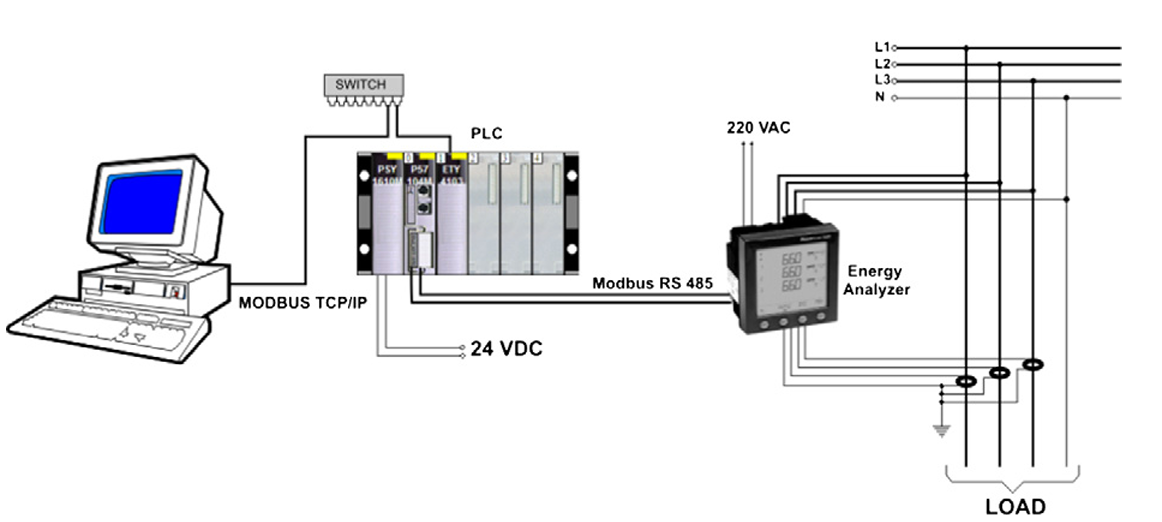
\includegraphics[width=0.8\columnwidth]{imgs/Schema of the proposed energy monitoring system.png}
    \caption[Short description for list of figures]{Schema of the proposed energy monitoring system }
    \label{fig-magnitude}
    \end{figure}%

    The reasons why Modbus-based energy monitoring systems are preferred are their open standard structure, easy expansion of the systems, compatibility with devices from different manufacturers, and low processing power requirements. Thanks to these systems, instant energy consumption in facilities can be monitored, measures can be taken to reduce consumption during peak load times, and overall energy efficiency can be increased. In addition, recording real-time consumption data allows for more accurate billing and the development of energy saving strategies by analyzing consumption habits.
    
    Advantages and disadvantages of Modbus communication protocol:
    \begin{table}[htbp]
        \centering
        \caption{Advantages and Disadvantages of Modbus Protocol}
        \begin{tabular}{|p{7cm}|p{7cm}|}
        \hline
        \textbf{Advantages} & \textbf{Disadvantages} \\
        \hline
        Open Standard: The Modbus protocol is free to use and compatible with devices from different manufacturers. &
        Limited data security: The Modbus protocol does not inherently have encryption or authentication mechanisms; extra security measures must be taken. \\
        \hline
        Easy integration: Many measuring devices can be easily connected to the network via RS-485 or TCP/IP infrastructure. &
        Slow data rate: Physical layers such as RS-485 offer low bandwidth, performance may be limited where very heavy data flow is required. \\
        \hline
        Low cost: Hardware and implementation costs are lower than other protocols. &
        Master-slave dependency: Due to the Modbus structure, only the master device initiates the query; the slave cannot send data on its own. \\
        \hline
        Wide industrial application: It has become the standard in many sectors such as power plants, factories, shopping malls, data centers. &
        Address limitation: Classic Modbus RTU networks have a theoretical limit of 247 devices. Larger networks require additional solutions. \\
        \hline
        \end{tabular}
        \label{tab:modbus_comparison}
        \end{table}
        



\section{Recommended Approaches}

As a real application, in the study titled "Automatic Meter Reading with LabVIEW Program for Real-Time Energy Monitoring and Consumer Awareness", a highly effective method has been developed in terms of energy saving and grid load balance. In the study, firstly, energy consumption data was collected instantly from smart meters installed in the field using RS-485 communication protocol. This data was processed with NI LabVIEW™ software and presented to consumers in a user interface both numerically and graphically. Thus, users were able to see their daily and instant energy consumption in detail and analyze their own consumption habits without waiting for billing periods. Not only monitoring software was used in the system infrastructure, but also a PLC unit was used to collect the data from the meters in a secure and regular manner, transfer them to the interface and monitor them. PLC played an active role in data communication in order to both collect the information obtained from the energy analyzers and facilitate real-time monitoring of the data. Thanks to this structure, the system has become more flexible, reliable and suitable for industrial use. In addition, different pricing strategies according to energy tariff slices have been integrated into the system design. Consumers are enabled to see the changes in energy prices instantly and thus are encouraged to prefer energy usage during lower tariff hours. In this way, not only individual energy savings but also the prevention of the load on the general network from concentrating during peak hours and a more balanced load distribution are provided. In the figure, the instant energy consumption values ​​collected from smart meters within the scope of the study carried out and the pricing information corresponding to these consumptions are reported in detail. The obtained data allows for real-time analysis of the consumption and cost relationship.



\begin{figure}[H]
    \centering
    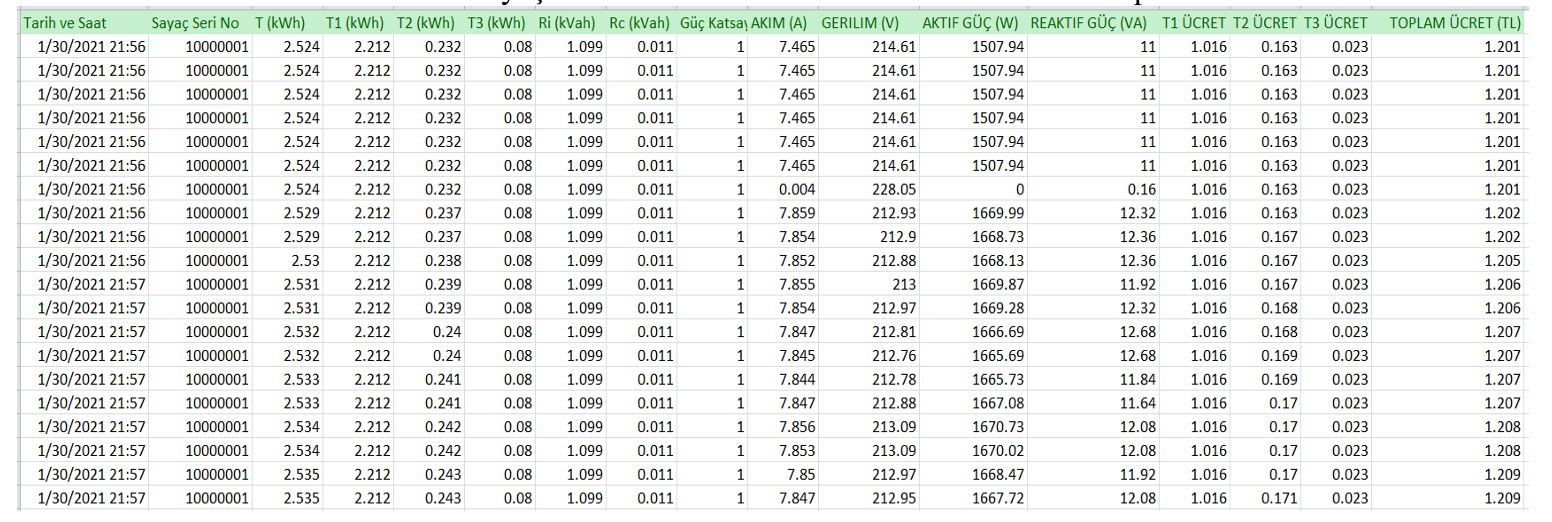
\includegraphics[width=0.8\columnwidth]{imgs/Report of Smart Meter Data in Excel Format.png}
    \caption[Short description for list of figures]{Report of Smart Meter Data in Excel Format }
    \label{fig-magnitude}
    \end{figure}%

    Another approach, "Integration of Modbus Ethernet Communication for Real-Time Electrical Power Consumption, Temperature, and Humidity Monitoring System", has been followed in order to solve the energy saving problem by using real-time data monitoring and management. In the study, electrical parameters such as voltage, current, power factor, as well as environmental variables such as temperature and humidity were collected from industrial energy analyzers. This data was recorded both locally and transferred to the cloud system via the ESP32 microcontroller. Thus, energy consumption and environmental conditions were continuously monitored, and early detection of abnormal consumption behaviors and environmental effects that would lead to loss of efficiency was provided. The measurement data obtained in the study was systematically categorized. In Table 1, data such as temperature, humidity, voltages, and currents collected from the devices used were recorded and analyzed in real time in Excel format. This data reveals the change in the temperature and humidity conditions of the electrical panel over time and the effect of this change on the energy parameters.

    \begin{figure}[H]
        \centering
        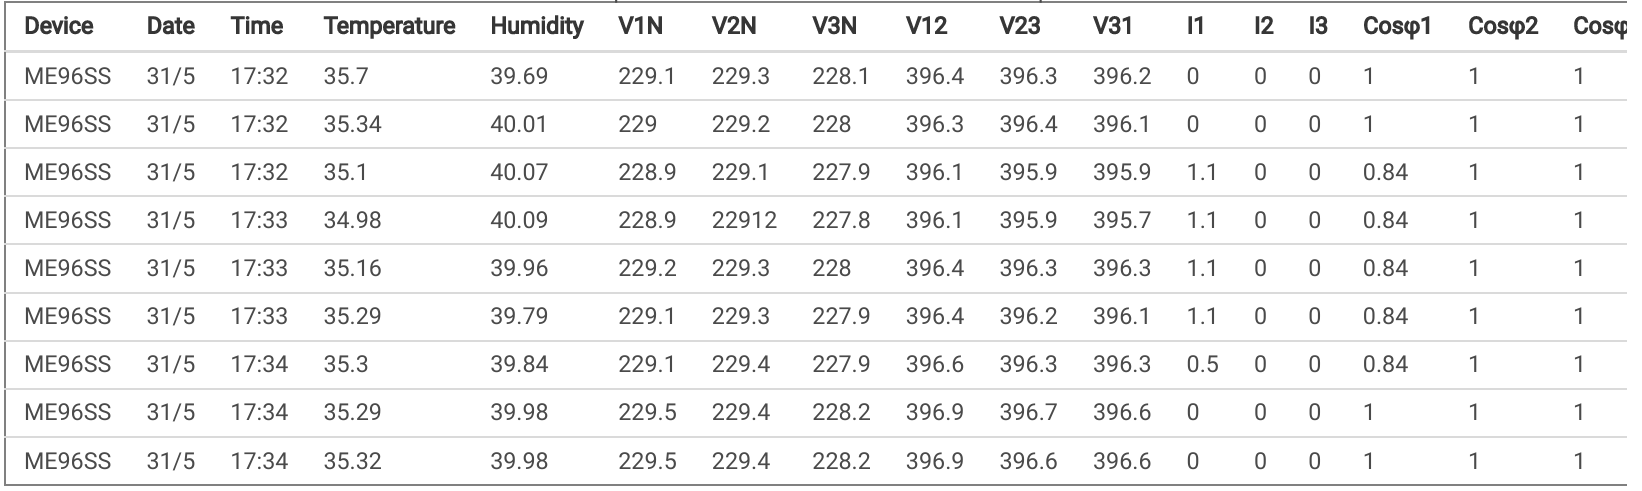
\includegraphics[width=0.8\columnwidth]{imgs/Electrical power data from the meter on the excel spreadsheet.png}
        \caption[Short description for list of figures]{Electrical power data from the meter on the excel spreadsheet }
        \label{fig-magnitude}
        \end{figure}%

        
\section{Induction Motor Energy Efficiency}

As part of a genuine literature review, the study titled “Energy Efficiency of Induction Motor Drives: State of the Art, Analysis and Recommendations” provides a detailed analysis of current approaches to improving the energy efficiency of induction motors. The authors systematically classified and analyzed 151 different literature studies in order to assess the current state of knowledge in this field.

The study emphasizes that despite global efforts to promote low-carbon energy sources, traditional fossil fuel-based systems still account for a high proportion of energy consumption. In this context, efforts to improve energy efficiency are coming to the fore. In particular, asynchronous motor drives, which are widely used in industry, account for a significant proportion of electrical energy consumption.

The study identifies five main and 48 sub-research areas aimed at improving energy efficiency and groups them under the following headings:

\begin{figure}[H]
    \centering
     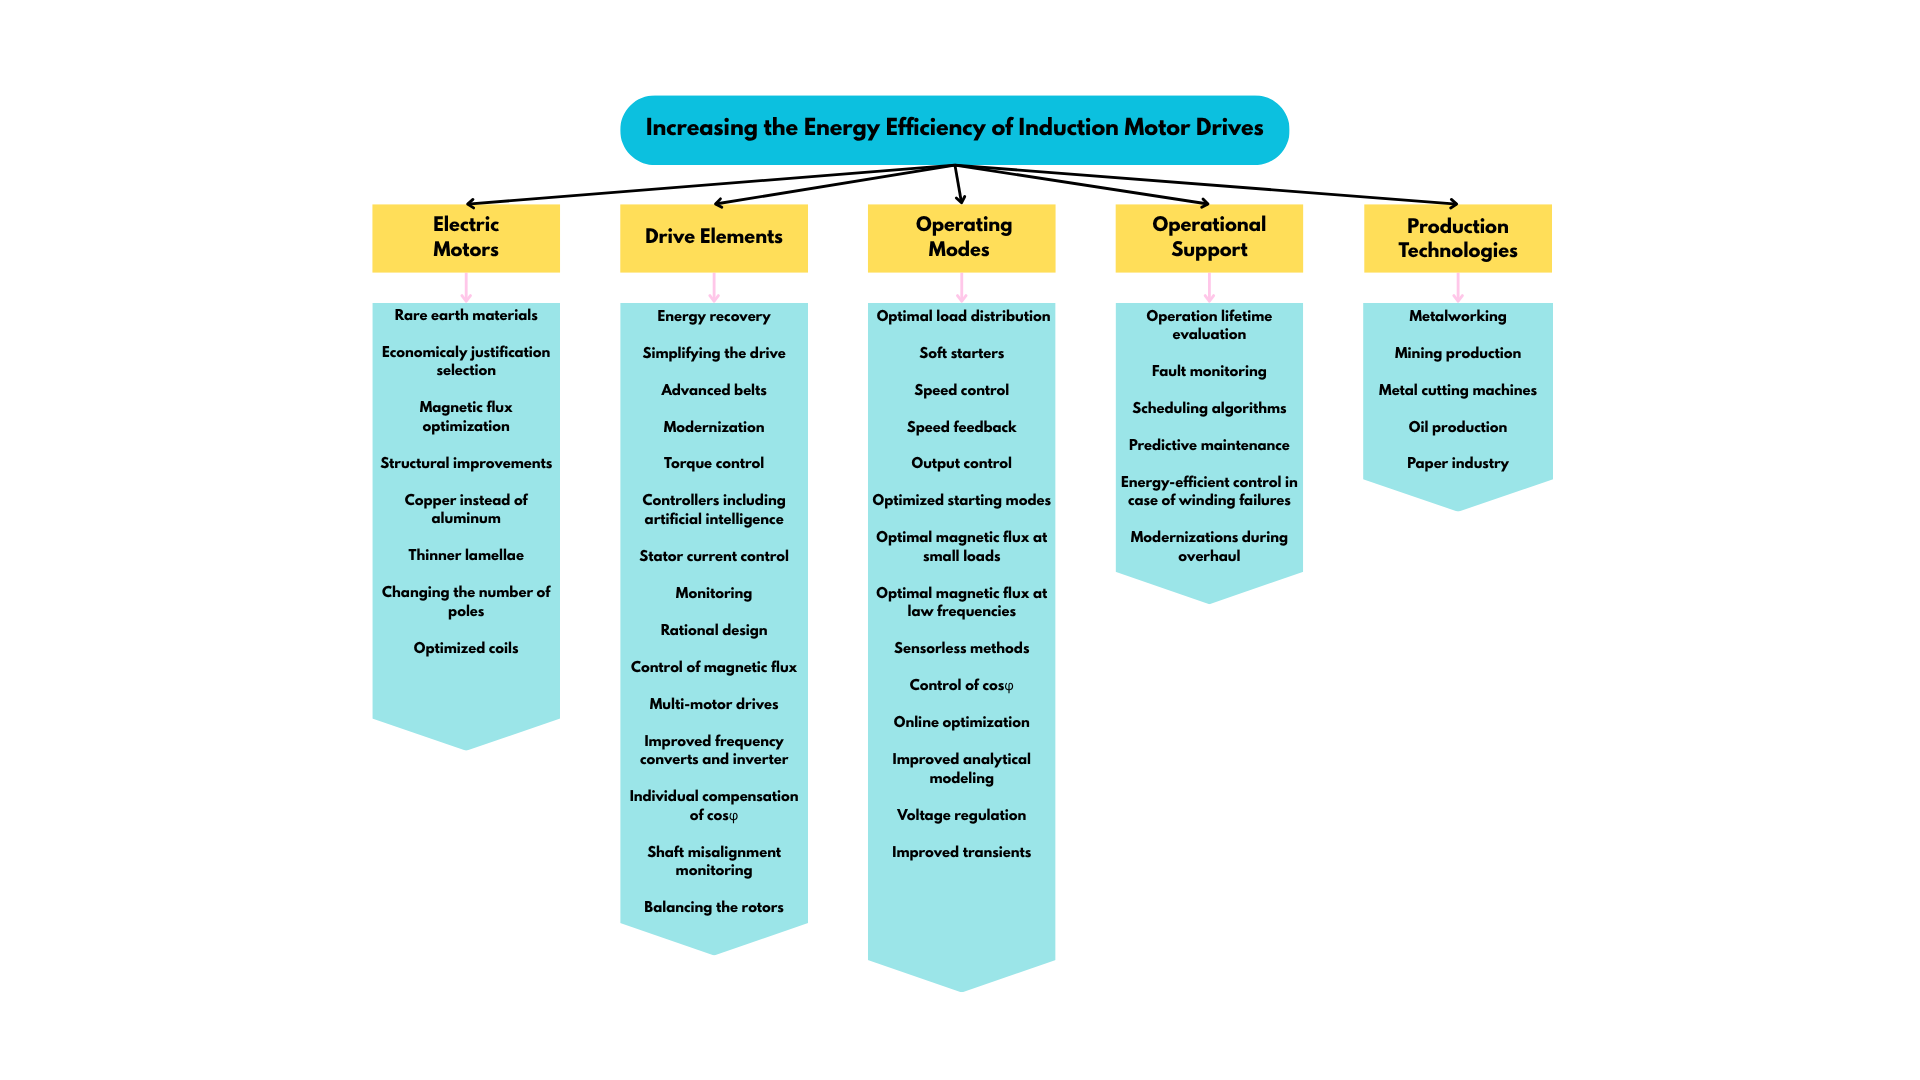
\includegraphics[width=0.8\columnwidth]{imgs/Optimal load distribution (1)} 
    \caption[Short description for list of figures]{Energy efficiency and Groups }
    \label{fig-magnitude}
    \end{figure}%

    


According to the analysis results, studies in the areas of “load distribution optimization” and “predictive maintenance” stand out in terms of the number of citations. However, it is also noted that factors such as field-based energy consumption measurements, the competencies of energy managers, and analyses of the current state of systems also play a decisive role in energy efficiency studies.

Based on the findings, it is recommended that future research prioritize issues such as the development of data collection systems, improving measurement accuracy, and creating decision support models for energy managers.

In this context, our study aims to optimize energy management through control strategies implemented on the operating mode of the asynchronous motor, thereby increasing the amount of energy saved. In line with this objective, it is planned to develop dynamic control algorithms suitable for the motor's load profile and operating conditions. This will ensure system-level efficiency and contribute to sustainability goals by reducing total energy consumption.


As part of a thorough literature review, the study titled “Endüstride Yüksek Verimli Motor Kullanımın Enerji Verimliliğine Etkileri” published by Üser et al. (2004) comprehensively examines the role of using high-efficiency motors in industry in reducing energy consumption. This study examines the energy savings and cost advantages of using high-efficiency motors instead of standard-efficiency motors in industrial facilities. The study details motor losses, efficiency calculation methods, and the technical characteristics of high-efficiency motors, and evaluates the performance of existing motors through applied measurements at Antalya ETİ Elektrometalurji A.Ş. The results indicate that transitioning to high-efficiency motors provides significant energy savings with a short payback period of approximately 19 months and offers an effective solution for improving energy efficiency in industrial facilities. The high cost of electricity compared to other energy types can provide significant cost advantages even when the savings rate is small. Electricity consumption in industrial facilities accounts for 10-25\% of total energy consumption, depending on the process, and in some cases, nearly 50\% of total energy costs are allocated to electricity. Therefore, electricity saving methods have the potential to significantly reduce total costs. Approximately 10\% of electricity consumption in industry is used for lighting and heating, while 90\% is used for electric motors. 95\% of these motors are alternating current short-circuit rotor asynchronous motors. Electric motors are used to convert electrical power into mechanical power. The fact that the majority of electrical energy in industry is consumed by motors highlights the critical importance of motor selection, operation, and maintenance in terms of energy savings.

{Losses Occurring When the Motor is Running Idle}: \\
When there is no load on the motor shaft, the rotor speed (nr) is close to the synchronous speed. The rotor speed is approximately 1\% less than the rotating field speed. In this case, the slip s is 1\%.

Asynchronous motors running at no load draw between 15\% and 50\% of their normal current (full load current) from the grid. When the motor is at no load, it draws the energy component of the current from the grid to compensate for the iron and friction losses of the stator and rotor. Additionally, it draws a certain amount of reactive component (magnetizing current). The motor's power factor at no load is low. The no-load losses can be summarized as follows: \\
• Iron losses (magnetic losses) are independent of load and remain constant.\\
• Friction (mechanical) losses are independent of load and remain constant. They may vary depending on motor speed.


Motor losses during load operation: \\
When the motor is idling, the slip amount s=1. When the load is applied, the rotor speed decreases and s increases. The cutting speed of the rotating field on the rotor windings increases. The electromotive force (emf) induced in the rotor increases. The phase currents increase. The current drawn from the grid by the motor increases. Accordingly, the losses under load can be listed as follows:\\
• Stator copper losses (primary $I^2R$ loss)\\
• Rotor copper losses (secondary $I^2R$ loss)\\
• Losses caused by load fluctuations

The energy loss rates that occur in the motors are given as percentages in Table 2.2.


\begin{table}[h!]
\centering
\begin{tabular}{|l|c|}
\hline
\textbf{Losses} & \textbf{\%} \\ \hline
Primary I\textsuperscript{2} losses & 5.6 \\ \hline
Secondary I\textsuperscript{2} losses & 2.7 \\ \hline
Core (iron) losses & 3.0 \\ \hline
Friction and windage losses & 1.4 \\ \hline
Losses due to load fluctuations & 2.3 \\ \hline
\textbf{TOTAL} & \textbf{15.0} \\ \hline
\end{tabular}
\caption{Ratios of Motor Losses}
\label{tab:losses}
\end{table}

Stator loss varies depending on stator current and resistance. The stator current expression is given in equation (2.1).

\begin{equation}
I_s = \frac{P_e}{\sqrt{3} \cdot U \cdot \cos\varphi}
\end{equation}

Here; $I_s$ is the stator current [A], $P_e$ is the electric power [W], 
$U$ is the voltage [V], and $\cos\varphi$ is the power factor. 
The rotor loss changes depending on the rotor resistance and $s$, 
and it is given in equation~(2.2).

\begin{equation}
\text{Rotor loss} = \frac{746 \cdot P_c \cdot f_w \cdot s}{1 - s}
\end{equation}


Here; $P_c$ is the output power in HP, $f_w$ is the total of friction 
and air friction losses, and $s$ is the motor slip. The rotor speed 
can never be equal to the synchronous speed of the poles $N_s$. 
In other words, the rotor speed is always less than the synchronous speed. 
There is always a slip.

Accordingly, the relationship between the speeds expressed by slip is shown in equation (2.3).

\begin{equation}
s = \frac{n_s - n_r}{n_s} \times 100
\end{equation}

The load-dependent variation of losses in an engine with up to 50 hp is shown in Figure 2.7.

\begin{figure}[H]
    \centering
    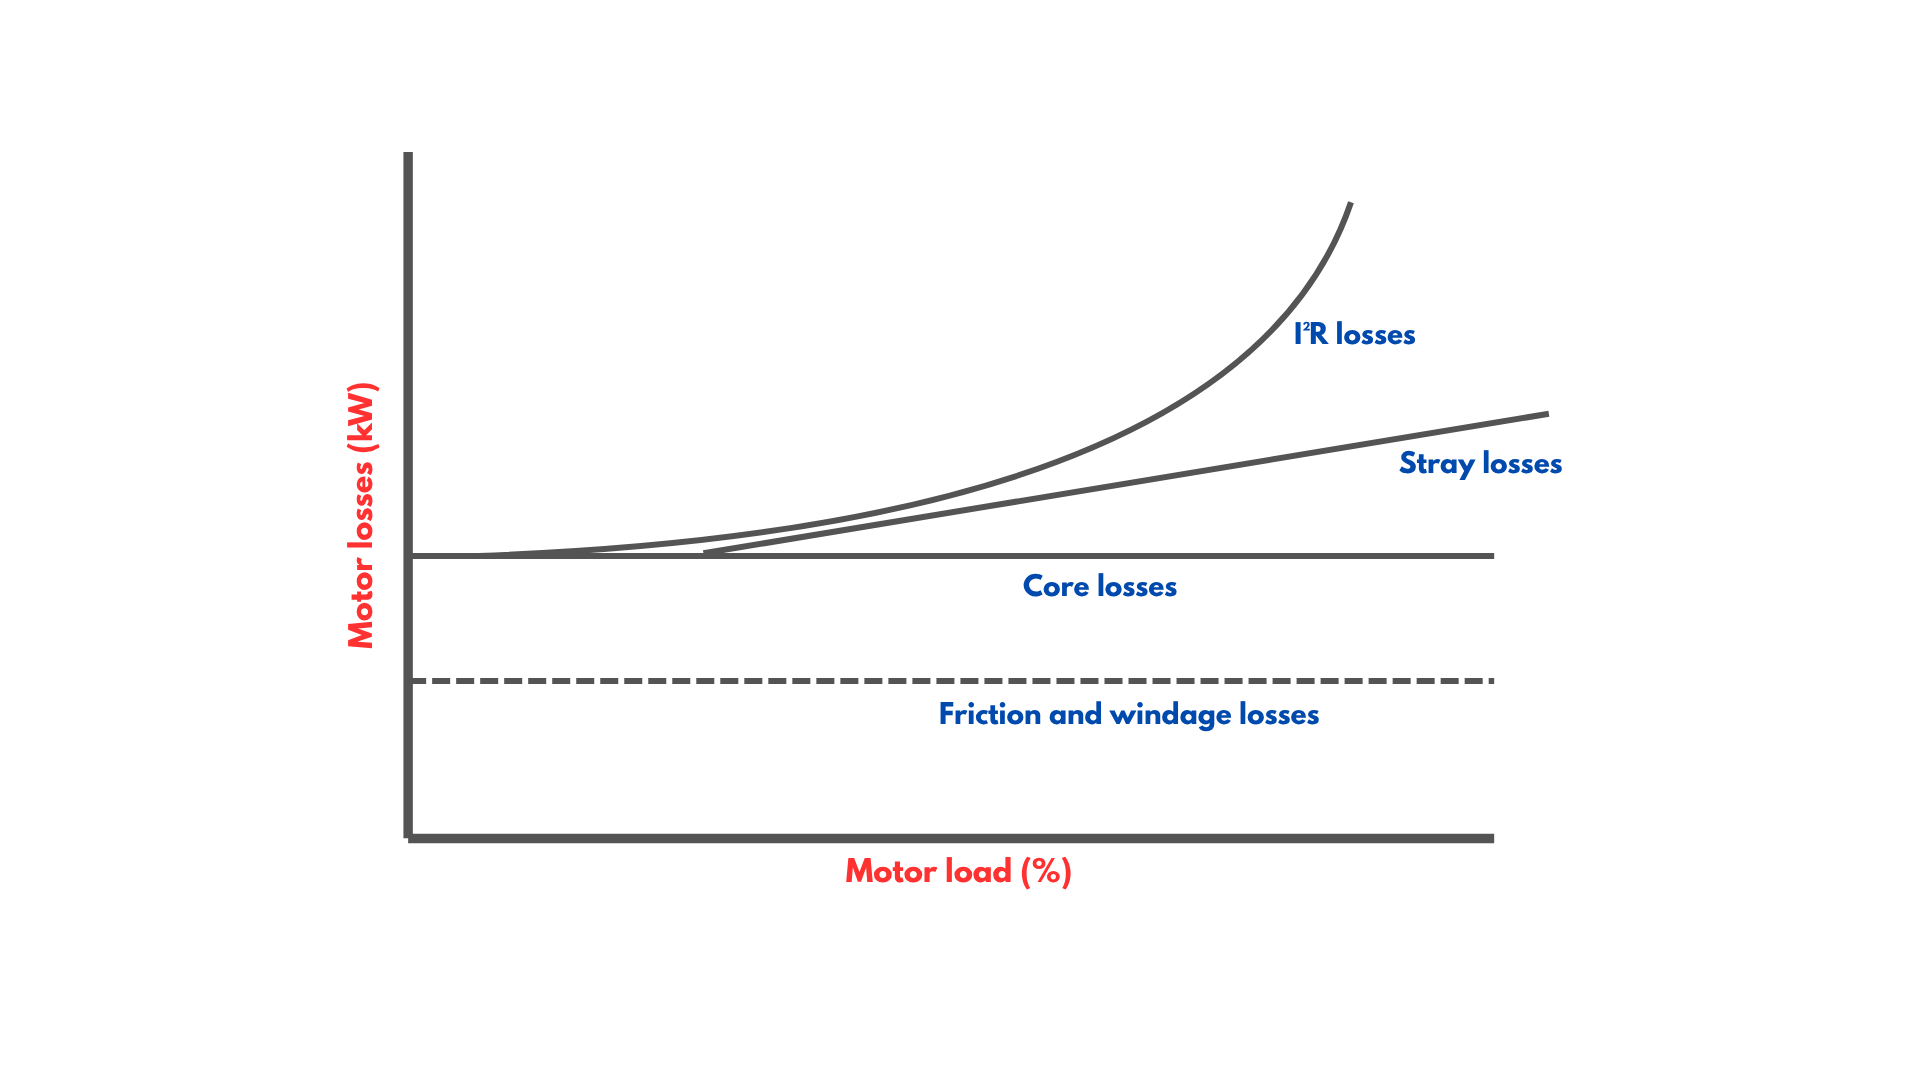
\includegraphics[width=0.8\columnwidth]{imgs/Motor losses (kW) (5).png}
    \caption[Short description for list of figures]{Changes in losses occurring in an engine up to 50 hp depending on the load }
    \label{fig-magnitude}
    \end{figure}%

In line with these theoretical foundations and experimental findings from the literature, our study focuses on applying targeted control strategies to manage the asynchronous motor’s operating modes in a way that minimizes unnecessary energy losses. By integrating real-time monitoring of motor load and slip with adaptive control algorithms, it becomes possible to dynamically adjust operating parameters to reduce copper, core, and mechanical losses. This approach not only aims to improve the overall efficiency of the motor system but also supports the long-term goals of industrial energy management by lowering operational costs and contributing to sustainability objectives.


In another study conducted by Çetin, Demir, and Çolak (2016) titled ''Energy Efficiency Analysis for Asynchronous Motors And Porsuk Vocational School Energy Efficiency Survey'', the high share of energy consumption and efficiency potential of three-phase squirrel cage asynchronous motors commonly used in industry were examined in detail. The study states that motor efficiency is the ratio of the power taken from the motor shaft to the electrical power consumed by the motor; efficiency losses are attributed to stator, rotor, iron, friction, and other losses. The information provided and the work conducted in the study are summarized as follows:

Electric motors are classified as direct current (DC) and alternating current (AC) motors. Ninety percent of electric motors used in industry are three-phase AC asynchronous motors, commonly referred to as squirrel cage motors. The reasons for this are their simple design, lower cost compared to other types, ease of maintenance, and the ability to connect directly to the AC grid. Therefore, the majority of energy is consumed by these motors. Significant energy savings can be achieved through energy efficiency studies on asynchronous motors. The use of high-efficiency electric motors is very important in reducing energy needs and costs. Efficiency in asynchronous motors is generally the ratio of the power taken from the motor shaft to the electrical power consumed by the motor. The difference between these two values represents the losses that are dissipated as heat energy and reduce motor efficiency. These losses are categorized as stator losses, rotor losses, iron losses, friction losses, and other losses. Today, these losses are being reduced, and higher energy-efficient asynchronous motors are being produced.

The first application based on efficiency in electric motors is the classification system adopted by CEMEP in 1998 to protect consumers and prevent unfair competition, known as EFF3, EFF2, and EFF1. This application covers motors ranging from 1.1 to 90 kW, with EFF3 being the lowest efficiency class and EFF1 the highest. In 2008, the International Electrotechnical Commission (IEC) published a new standard for efficiency classes, which became a European standard in 2009 and was adopted by the Turkish Standards Institute in 2010. These new efficiency classes are defined as IE1, IE2, IE3, and IE4. The IEC 60034-2-1 standard specifies the rules for motor efficiency testing methods, while the IEC 60034-30 standard explains the efficiency classes for electric motor groups directly powered by the grid. With the implementation of the IEC 60034-30-1 standard in 2014, the highest efficiency class became IE4, and the scope of efficiency was expanded. The IEC 60034-30-1 standard defines four IE (international efficiency) classes for all electric motors classified for sinusoidal voltage. According to this standard, efficiency classes are defined as shown in Table 2.3.

\begin{table}[h!]
\centering
\begin{tabular}{|l|c|}
\hline
\textbf{Standard Efficiency} & IE1 \\ \hline
\textbf{High Efficiency}   & IE2 \\ \hline
\textbf{Premium Efficiency}  & IE3 \\ \hline
\textbf{Super Premium Efficiency } & IE4 \\ \hline
\end{tabular}
\caption{Efficiency Classes}
\end{table}

The efficiency classes specified above apply to motors with a power rating between 0.75 kW and 375 kW, operating at frequencies of 50 and 60 Hz, and voltages up to 1000 V. The efficiency class of the motors is determined using the test methods specified in the IEC 60034-2-1 standard. The minimum efficiency value and the corresponding IE class of the manufactured motors must be indicated on the motor nameplates. An example of a motor nameplate is provided in Figure 2.8.

\begin{figure}[H]
    \centering
    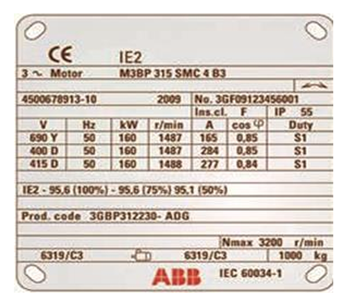
\includegraphics[width=0.6\columnwidth]{imgs/motor etiket resmi.png}
    \caption[Short description for list of figures]{Sample Motor Nameplate }
    \label{fig-magnitude}
    \end{figure}%

At the Vocational School, there are a total of 19 electric motors used for processes such as hot water transfer, irrigation, and circulation. An energy audit of these motors was carried out to find out how much energy could be saved and how long it would take for the investment cost to be recovered if the existing motors were replaced with high-efficiency motors. As a result of the inspections, the number and features of the motors used are shown in the table below.

\begin{table}[h!]
\centering
\begin{tabular}{|c|c|c|}
\hline
\textbf{Number of Engines} & \textbf{Engine Power (kW)} & \textbf{Motor Rotation Speed (rpm)} \\ \hline
11 & 0,55 & 3000 \\ \hline
5  & 1,50 & 3000 \\ \hline
2  & 1,50 & 1500 \\ \hline
1  & 0,75 & 1500 \\ \hline
\end{tabular}
\caption{Current Motor Information at School}
\end{table}

$P$ = Power ratings of the motors used (kW),\\
$\eta_1$ = Efficiency value of the old motors (\%),\\
$\eta_2$ = Efficiency value of the new motors (\%),\\
$n$ = Number of motors,\\
$t$ = Motor operating time (h),\\
$\alpha$ = Energy cost per hour (Eur/kWh)\\

Using these definitions, the calculations are performed with Equation~\ref{eq:1} and Equation~\ref{eq:2}, and the results are examined in Table~5 in the results section.

\begin{equation}
\label{eq:1}
\text{Annual Saving from Replacement} = (P \times \eta_1 - P \times \eta_2) \times \alpha \times t \times n
\end{equation}

\begin{equation}
\label{eq:2}
\text{Payback Period (Years)} = \frac{\text{Total Replacement Cost}}{\text{Annual Saving from Replacement}}
\end{equation}

In the calculations, the annual usage of the motors was assumed to be 4320 hours, and the unit cost of electricity was assumed to be 0.07 Eu/kWh. The review revealed that the motors had not been rewound previously, so the efficiency loss due to rewinding was not included in the calculation. The calculations were based on the efficiency of the motors at 100\% load (Direct Online). For motors currently in operation, the efficiency values of the motors were accepted as IE1 values defined in the IEC/EN 60034 30-1: 2014 standard. New motors were selected from the IE3 efficiency class due to the unavailability of IE4 motor production at current power levels and were included in the calculations at current purchase prices.

The issue of how to achieve efficiency and savings in asynchronous motors, which consume large amounts of electrical energy, has been addressed in conjunction with analyses of pump motors at the Vocational High School. Given the difficulties involved in generating electrical energy, it is clear that we must use it efficiently. The goal of efficient use is to reduce losses, consume less energy in production processes, provide savings to individuals or companies, and contribute to the national economy and environmental protection. Humanity's consumption of electrical energy is increasing faster than primary energy consumption, and this increase is occurring even more rapidly in our country due to our status as a developing nation. Therefore, electricity conservation should be given utmost importance, and awareness should be raised. As mentioned earlier, nearly half of total electricity consumption occurs in electric motors. Among these, pump systems account for 20\% of consumption. Therefore, implementing a high-efficiency design in pump systems would result in significant savings.

\begin{table}[h!]
\centering
\resizebox{\textwidth}{!}{%
\begin{tabular}{|c|c|c|c|c|c|c|c|c|c|c|c|}
\hline
\textbf{No} & \textbf{Process} & \textbf{Power (kW)} & \textbf{Speed (rpm)} & \textbf{Motor Qty} & \textbf{IE3 Eff.} & \textbf{Old Eff.} & \textbf{Annual Operating Hours} & \textbf{Annual Saving (EUR)} & \textbf{Motor Unit Price (EUR)} & \textbf{Total Replacement Cost (EUR)} & \textbf{Payback Period (Years)} \\ \hline
1 & Pump & 0.55 & 3000 & 11 & 0.772 & 0.658 & 4320 & 410.58 & 90 & 990 & 2.41 \\ \hline
2 & Pump & 1.50 & 3000 & 5  & 0.825 & 0.752 & 4320 & 266.87 & 130 & 650 & 2.44 \\ \hline
3 & Pump & 1.50 & 1500 & 2  & 0.853 & 0.772 & 4320 & 111.59 & 140 & 280 & 2.51 \\ \hline
4 & Pump & 0.75 & 1500 & 1  & 0.825 & 0.721 & 4320 & 39.65  & 105 & 105 & 2.65 \\ \hline
\textbf{Total} &  &  &  &  \textbf{19}&  &  &  & \textbf{828.69} &  & \textbf{2025} & \textbf{2.44} \\ \hline
\end{tabular}%
}
\caption{Porsuk Vocational School Electric Motor Analysis Results}
\end{table}

Each row of the efficiency calculation table contains the motor power and speed for the relevant process, IE1 efficiency values accepted according to IEC standards and new motor IE3 efficiency values, total operating hours of motors per year, annual savings achieved through energy savings, unit and total replacement costs of motors, and finally, the payback period of the investment. Process 1 has 11 asynchronous motors operating at 0.55 kW and 3000 rpm. The current motor efficiency values are accepted as IE1 at 65.8\%, and the recommended replacement motors are selected with an efficiency value of IE3 at 77.2\%. When calculated assuming that the motors operate for 4,320 hours annually, the efficiency improvement results in a total annual savings of 410.58 EUR for the 11 motors. The unit price of the new IE3-class motors is 90 EUR, resulting in a total investment cost of 990 EUR. When comparing the total investment cost to the annual savings, the payback period for the change is calculated to be 2.41 years.In process 2, replacing five 1.5 kW 3000 rpm motors with IE3 efficiency class motors instead of IE1 efficiency class motors results in an annual savings of 266 EUR. This recoups the total motor replacement cost of 650 EUR in 2.44 years. In Process 3, replacing two motors with a power rating of 1.5 kW and a speed of 1500 rpm results in an annual savings of 111.59 EUR. This recoups the replacement cost of 280 EUR in 2.51 years. In process number 4, the replacement of one motor with a power of 0.75 kW and a speed of 1000 rpm yields an annual savings of 39.65 EUR. As a result, the investment cost of 105 EUR is recovered in 2.65 years. In conclusion, a study conducted to improve motor efficiency classes in the system results in a total investment cost of 2025.00 EUR. As seen in the table calculations, improving motor efficiency values can result in annual energy savings of 828.69 EUR. This means that the total investment cost can be recovered in an average of 2.44 years, and significant savings can be achieved over the operational lifespan of the motors.

The connection between this study and our study is that both studies share the common goal of increasing energy efficiency. While the aforementioned research aims to achieve savings through the selection and replacement of high-efficiency motors on the hardware side, our study aims to achieve energy management through real-time monitoring of operating modes and optimization using control algorithms in existing asynchronous motors. Thus, in addition to approaches requiring hardware modernization, similar levels of efficiency gains and short payback periods can be achieved through control and monitoring-based strategies.

Kapsamlı bir literatür taramasının parçası olarak ele alınan “Design and Implementation of PLC-based Monitoring Control System for Induction Motor” başlıklı çalışma,elektrik tahrik sistemlerinde hareket kontrol teknolojilerinin gelişmesiyle birlikte, programlanabilir lojik kontrolörlerin (PLC) güç elektroniğiyle entegre kullanımının sanayi otomasyonunda sağladığı avantajları vurgulamaktadır. PLC’ler sayesinde motor kontrolü yüksek güç faktörü ile yapılabilir, üretim maliyetleri düşer ve sistem güvenilirliği artar. Literatürde DC makineler, step motorlar, relüktans motorlar ve lineer motorlar gibi çeşitli motor tiplerinin PLC ile kontrolüne yönelik çalışmalar bulunmakla birlikte, asenkron motorların PLC ile kontrolü üzerine yapılan yayınlar sınırlıdır. Bu makale, üç fazlı asenkron motor için PLC tabanlı izleme ve kontrol sisteminin tasarımını, donanım-yazılım entegrasyonunu ve test sonuçlarını sunmaktadır.
PLC; mikroişlemci tabanlı, endüstriyel ortamlarda otomasyon süreçleri için tasarlanmış bir kontrol sistemidir. Giriş/çıkış modülleri aracılığıyla sensörlerden veri alır ve aktüatörlere komut gönderir. Çalışmada kullanılan PLC modüler yapıdadır: CPU, güç kaynağı, dijital giriş/çıkış modülleri, analog giriş/çıkış modülleri ve programlama terminalinden oluşur. Bu yapı, ileride çoklu motor sistemleri veya bilgisayar bağlantısı gibi genişletmeler için esnek bir çözüm sunar.\\
\\
Deneysel sistem (Şekil 2.7), üç farklı modda çalışacak şekilde tasarlanmıştır:\\
    • Kapalı çevrim sabit hız kontrolü – hız ve yük akımı geri beslemeleri kullanılır, inverter çıkışı PLC tarafından kontrol edilir.\\
    •Açık çevrim değişken hız kontrolü – PLC devre dışı bırakılır, inverter sabit kontrol modunda çalışır.\\
    •Standart sabit gerilim–sabit frekans çalışması – kontrol sistemi tamamen devre dışı bırakılır.\\
\begin{figure}[H]
    \centering
    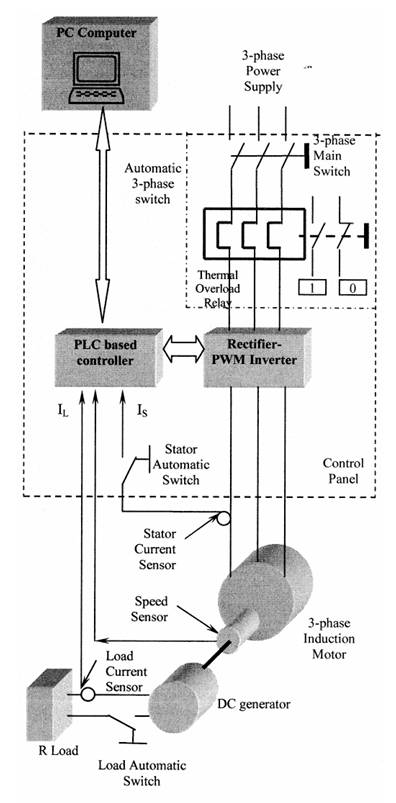
\includegraphics[width=0.4\columnwidth]{imgs/Electrical diagram of experimental system.png}
    \caption[Short description for list of figures]{Electrical Diagram of Experimental System }
    \label{fig-magnitude}
    \end{figure}%

Sistem, sarılı rotorlu asenkron motor (Tablo 2.6) ve değişken yük sağlayan DC jeneratörden oluşmaktadır. Üç fazlı güç kaynağı ana şalter, termik röle ve doğrultucu üzerinden IGBT tabanlı invertere bağlanmıştır. İnverter, DC gerilimi üç fazlı AC’ye dönüştürerek motorun statoruna uygular. PLC’ye bağlı hız sensörü (takogeneratör) ve akım sensörleri ile kapalı çevrim geri beslemeler sağlanmıştır. Kontrol panelinde anahtarlar, butonlar, sinyal lambaları ve seçiciler ile birlikte tüm modüller yer almaktadır.

\begin{table}[h!]
\centering
\label{tab:induction_motor_specs}
\begin{tabular}{|l|c|}
\hline
\textbf{Connection type} & $\Delta$/Y \\ \hline
\textbf{Input voltage} & 380/660 V ac \\ \hline
\textbf{Input current} & 1.5/0.9 A \\ \hline
\textbf{Rated power} & 0.6 kW \\ \hline
\textbf{Input frequency} & 50 Hz \\ \hline
\textbf{Pole number} & 4 \\ \hline
\textbf{Rated speed} & 1400 rpm \\ \hline
\end{tabular}
\caption{Induction Motor Technical Specifications}
\end{table}

\begin{table}[h!]
\centering
\label{tab:inverter_specs}
\begin{tabular}{|l|l|}
\hline
\textbf{Output voltage} & 380, 460 V ac \\ \hline
\textbf{Output frequency} & 0, 480 Hz \\ \hline
\textbf{Output current} & 2.5 A \\ \hline
\textbf{Output overload} & 150\% for 60 s \\ \hline
\textbf{Power supply voltage} & 380, 460--10\% V ac \\ \hline
\textbf{Input current} & 3 A \\ \hline
\textbf{Dissipated power} & 46 W \\ \hline
\end{tabular}
\caption{Inverter Technical Specifications}
\end{table}

Aşırı akım rölesinin çıkışı, üç fazlı gerilimi doğru akıma çeviren bir **doğrultucu (rectifier)**ya bağlıdır. Elde edilen doğru akım, yalıtılmış kapılı bipolar transistör (IGBT) tabanlı bir invertere giriş olarak verilir. İlgili teknik özellikler Tablo 2.7’de özetlenmiştir. Bu inverter, DC gerilimi tekrar üç fazlı AC gerilime çevirerek motorun stator sargılarına uygular.

Kontrolör, modüler tip bir PLC sistemi üzerine kurulmuştur. PLC donanımı şu temel modüllerden oluşmaktadır:\\
Merkezi İşlem Birimi (CPU): Programı çalıştırır, veri işlemlerini ve giriş/çıkış kontrolünü yönetir.\\
Dijital Çıkış Modülü (DOM) ve Dijital Giriş Modülü (DIM): Motorun çalıştırılması, durdurulması ve yön kontrolü gibi fonksiyonları sağlar.\\
Analog Giriş Modülü (AIM): Hız ve yük akımı sensörlerinden gelen sinyalleri alır.\\
Analog Çıkış Modülü (AOM): İnverterin kontrol sinyallerini üretir.
Güç Kaynağı Ünitesi: PLC’nin tüm modüllerine gerekli DC beslemeyi sağlar.\\

Sistem, iki geri besleme döngüsüne sahiptir:\\
Hız geri beslemesi: Motorun miline bağlı bir takogeneratör (kalıcı mıknatıslı DC motor) ile sağlanır. Takogeneratör çıkış voltajı motor devrine orantılıdır ve AIM modülü tarafından okunur.\\
Yük akımı geri beslemesi: Motor çıkışına bağlanan akım sensörü ile elde edilir.

Manuel kontrol için sistemde; başlatma, durdurma, trip butonları; ileri/geri yön seçim anahtarı; hız seçici ve kazanç ayar anahtarı bulunmaktadır. Kontrol paneli üzerinde ayrıca; ana şalter, otomatik üç fazlı şalter, otomatik tek fazlı şalter, aşırı yük rölesi, yük şalteri, sinyal lambaları ve PLC modülleri yer almaktadır. Program, kişisel bilgisayardan PLC’ye RS232 seri arayüz üzerinden yüklenmektedir.

PLC programı merdiven diyagramı (ladder diagram) yöntemi ile geliştirilmiş, RS232 üzerinden yüklenmiştir. Program; giriş sinyallerini izler, çıkışları kontrol eder ve hız–akım geri beslemelerine göre inverteri yönetir. PLC bellek yapısı giriş, çıkış ve veri bölgelerine ayrılmıştır. Kapalı çevrim kontrol algoritması ile yük değişimlerine rağmen hızın sabit tutulması sağlanmıştır.


\begin{figure}[H]
    \centering
    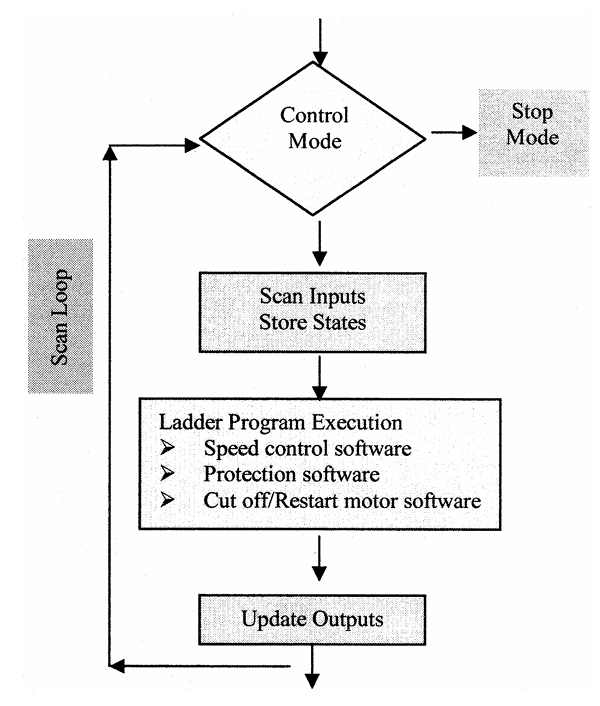
\includegraphics[width=0.4\columnwidth]{imgs/Flowchart of the main program..png}
    \caption[Short description for list of figures]{Flowchart of the Main Program}
    \label{fig-magnitude}
    \end{figure}%

Testler, PLC tabanlı kapalı çevrim kontrolün, geleneksel V/f kontrolüne göre daha yüksek hız doğruluğu sağladığını göstermektedir. Senkron hızın \%95’ine kadar verim korunmuş, değişken yük altında dahi hız sapmaları minimum seviyede kalmıştır. 

\begin{figure}[H]
    \centering
    \includegraphics[width=0.4\columnwidth]{imgs/Experimental speed–torque characteristics with PLC and inverter.png}
    \caption[Short description for list of figures]{Experimental Speed–Torque Characteristics with PLC and Inverter}
    \label{fig-magnitude}
    \end{figure}%

Şekil 7 (Deneysel hız-tork karakteristikleri): PLC ve inverter kontrolü altındaki motorun farklı referans hızlarda (600, 900, 1225, 1400 rpm) tork değişimine karşı hız tepkisini net şekilde gösteriyor. Bu, sistemin dinamik yük altında hız regülasyonu performansını karşılaştırmak için kritik.

Bu makaledeki PLC tabanlı kontrol sistemi, yük değişimlerinde motor hızını sabit tutma başarısıyla öne çıkıyor. Deneysel sonuçlarda, özellikle yüksek hızlarda, PLC kontrolünün yalnızca invertere kıyasla hız düşüşünü önemli ölçüde azalttığı görülüyor. çalışmamızda ise asenkron motorun çalışma modunu gerçek zamanlı izleyip yük ve kayma değerlerine göre adaptif şekilde kontrol ederek gereksiz enerji kayıplarını minimize etme hedefi var. Bu iki yaklaşım temelde aynı prensibe dayanıyor: motorun hız ve tork davranışını hassas şekilde kontrol ederek hem performans hem de enerji verimliliğini artırmak.

\begin{figure}[H]
    \centering
    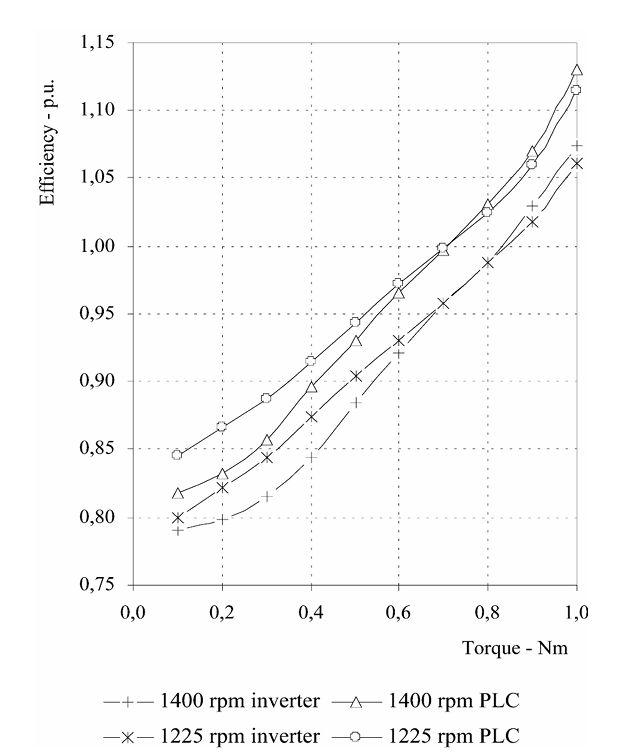
\includegraphics[width=0.4\columnwidth]{imgs/Efficiency of controlled system with and without PLC per unit of efficiency of standard supplied motor..png}
    \caption[Short description for list of figures]{Efficiency of Controlled System with and without PLC per unit of Efficiency of Standard Supplied Motor.}
    \label{fig-magnitude}
    \end{figure}%

PLC kontrollü ve yalnızca inverter kontrollü sistemlerde verimliliğin torka bağlı değişimini sunuyor. Enerji yönetimi ve verimlilik optimizasyonu açısından doğrudan kıyaslama imkânı veriyor.

\section{Gaps and Limitations}

Literature reviews show that significant progress has been made in both Modbus-based energy monitoring systems and studies aimed at improving energy efficiency in asynchronous motors. However, when previous studies are examined, some common shortcomings are apparent. Firstly, Modbus-based energy monitoring applications are mostly limited to measurement, data collection, and visualization; there is insufficient focus on analyzing the collected data in real time and integrating it into motor control algorithms, i.e., transforming it into a closed-loop structure that directly provides energy optimization. This situation limits the potential energy savings capacity of the systems. On the other hand, most studies on asynchronous motor efficiency focus on hardware-based improvements (high-efficiency motor selection, motor replacement, mechanical improvements, etc.); methods for achieving energy savings without hardware changes in the existing motor fleet, using only software-based control strategies, are addressed in a limited number of cases.Furthermore, many of these studies did not take into account different load profiles, variable operating conditions, and industrial driving cycles; optimization was generally tested under constant load or laboratory conditions. Another limitation is that secondary loss components such as thermal effects, harmonic distortion (THD), and voltage imbalances are not integrated into energy management algorithms in motor efficiency analyses. In field studies focused on high-efficiency motor use, while payback periods and cost analyses are presented in detail, an integrated analysis directly comparing these scenarios with control-based software solutions is lacking. Therefore, while the existing literature provides significant knowledge on energy monitoring and motor efficiency, there is a need for comprehensive studies that combine real-time monitoring data with control algorithms, adaptively respond to different load and environmental conditions, and comprehensively compare both hardware and software-based solutions.

\section{Justification for Proposed Approach}

Modbus-based energy monitoring systems, which are widely used in industrial facilities today, ensure accurate and real-time monitoring of electrical parameters (current, voltage, power, energy consumption, etc.). However, it is not common practice to integrate this data directly into motor control algorithms to increase energy efficiency. A review of the current literature reveals that a significant portion of energy efficiency studies focus on hardware-based approaches, particularly high-efficiency motor selection and motor replacement, while the topic of achieving energy savings in existing motor fleets through software and control algorithms is addressed only to a limited extent. However, in many industrial facilities, motor replacement is not feasible in the short term due to factors such as cost, downtime, and integration challenges. At this point, real-time monitoring of the operating modes and load profiles of existing motors, combined with the application of adaptive control strategies based on the data obtained, offers significant energy savings potential without the need for hardware changes. The proposed approach aims to dynamically optimize the motor's operating mode by analyzing real-time motor data collected via Modbus RTU/TCP in terms of parameters such as load, slip, temperature, and power factor. This will reduce unnecessary copper, iron, and mechanical losses, and by operating the motor only at the required torque and speed levels, both energy consumption will be reduced and equipment lifespan will be extended. This method, as a low-cost software-based solution, can provide similar efficiency increases to methods requiring hardware modernization, offer industrial-scale applicability with short payback periods, and contribute to sustainability in the field of energy management.  


\clearpage
\doublespacing % Do not change - required

\chapter{ Methodology}
\label{ch3}

%%%%%%%%%%%%%%%%%%%%%%%%%%%%%%%%%%%%%%%
% IMPORTANT
\begin{spacing}{1} %THESE FOUR
\minitoc % LINES MUST APPEAR IN
\end{spacing} % EVERY
\thesisspacing % CHAPTER
% COPY THEM IN ANY NEW CHAPTER
%%%%%%%%%%%%%%%%%%%%%%%%%%%%%%%%%%%%%%%



\section{Programmable Logic Controller (PLC)}

PLC is a control device that enables processes to be managed safely, efficiently and flexibly in industrial automation systems. Dick Morley is an electrical engineer known as the father of PLC. Morley is the founder and president of Bedford Associates, where he created Modicon in 1968. PLC was first used in General Motors factories. PLCs, which can control automation elements such as sensors, buttons, motors, relays and contactors through input-output modules, offer advantages such as taking up less space, having fewer failures and performing faster processes compared to classic relay systems. For these reasons, they have replaced traditional relay systems over time.

\begin{figure}[H]
    \centering
    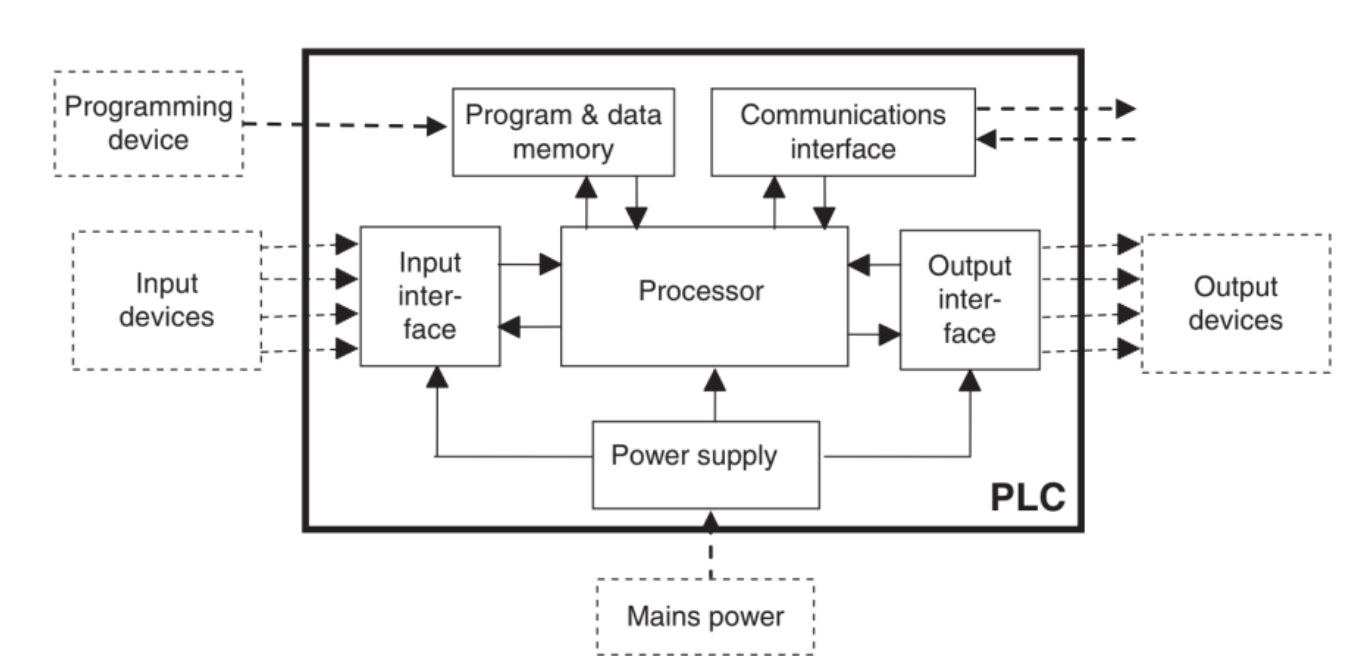
\includegraphics[width=0.8\columnwidth]{imgs/The PLC system.png}
    \caption[Short description for list of figures]{The PLC system }
    \label{fig-magnitude}
    \end{figure}%


    The basic components of the PLC include the Central Processing Unit (CPU), Memory Unit, Input-Output (I/O) Unit, Signal Compatibility Circuits and Expansion Modules. The CPU is the management center of the system and performs arithmetic and logical operations by processing the signals it receives from the input units, then controls the automation processes by transmitting the appropriate commands to the output units. Basic functions such as Timer, Counter and Comparator are operated within the CPU in order to perform the specified process flows. The Memory Unit, which determines the operating logic of the CPU, allows the storage of program codes and process data. In this context, RAM stores temporary data, while ROM and EPROM ensure that the program is protected in the event of a power outage and rewritten when necessary. This structure increases the flexibility and long-term operational sustainability of the system. The Input-Output (I/O) Unit is the main component that enables the PLC to exchange data with the physical world. Input modules receive analog or digital signals from sensors, buttons, and switches and convert them into digital data formats that the CPU can process. Output modules convert the commands processed by the CPU into appropriate electrical signals that will operate actuators such as motors, relays, and solenoid valves. Signal Compatibility Circuits in the system regulate the voltage levels of signals coming from/going to input and output units, provide protection, and enable the PLC to communicate safely with different system components.

    \begin{figure}[H]
        \centering
        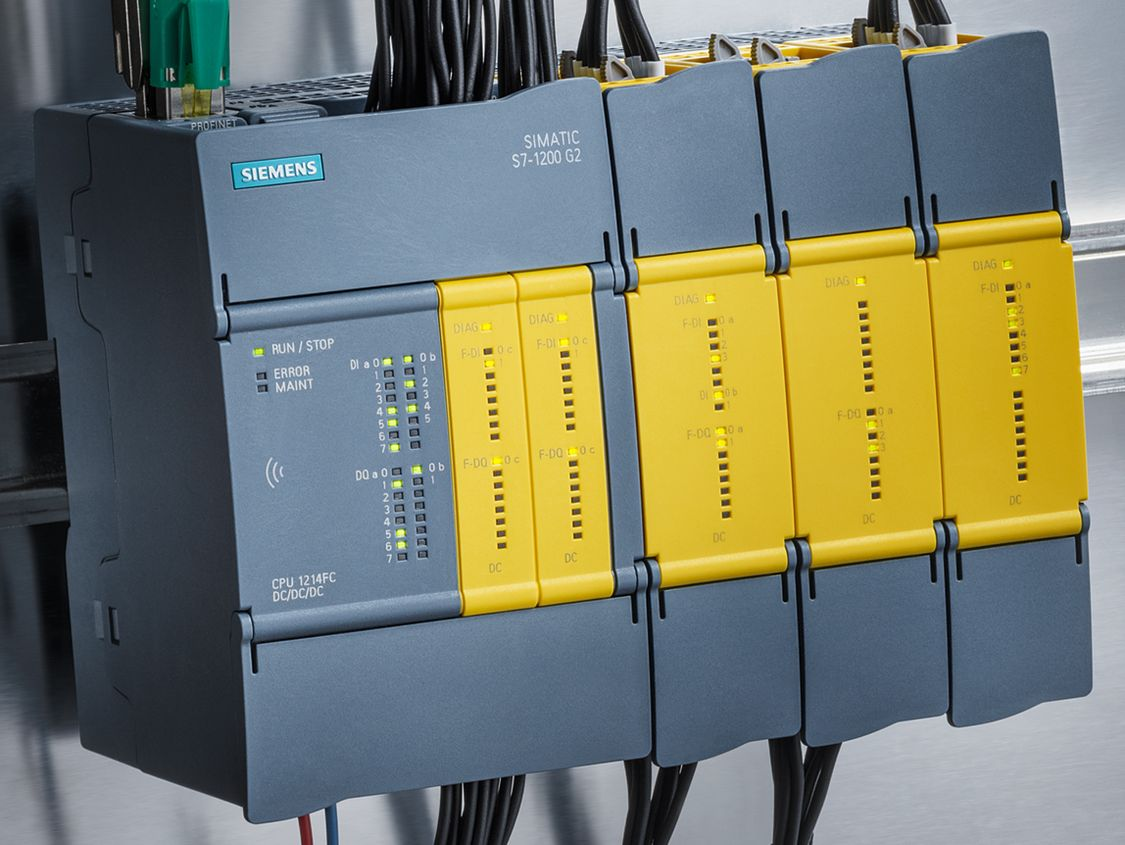
\includegraphics[width=0.8\columnwidth]{imgs/SIMATIC-S7-1200-G2.jpg}
        \caption[Short description for list of figures]{SIMATIC-S71200 }
        \label{fig-magnitude}
        \end{figure}%   
    
        In our study, Siemens S7-1200 series PLC model was preferred. Siemens S7-1200 is a common programmable logic controller (PLC) model that offers expandability thanks to its modular structure, operates with 24V DC supply voltage and provides high-speed switching capability via digital input-output modules and transistor outputs. Its compatibility with communication protocols such as Modbus and Profinet facilitates integration with different automation systems; and thanks to its high resistance to harsh environmental conditions, it offers a wide range of applications from industrial facilities to energy management systems. The CPU 1214C model of the series offers a reliable and scalable control solution in industrial areas such as automatic production lines, process control systems, building automation and energy management with its fast processing capacity, comprehensive communication protocol support and robust structure; It is effectively used in applications requiring high performance.



       
\section{Modbus}

Modbus is one of the oldest and most common protocols that provide communication between PLCs and other industrial devices. It was developed by Modicon in 1978 and over time it has become a standard communication method that provides data transfer and information exchange between PLC systems.

Modbus, which works with the master-slave model, has been divided into different versions such as Modbus RTU and Modbus TCP over time. While Modbus RTU is based on serial communication, Modbus TCP is TCP/IP based. While the PDU (Protocol Data Unit) is fixed in data transmission and works independently of the lower layer, the content of the Modbus ADU (Application Data Unit) changes according to the type of protocol used. Figure 5 shows the structure of the Modbus ADU and Modbus TCP/IP ADU data packets. Modbus RTU and Modbus ASCII use serial communication (RS-232, RS-485) and the ADU structure consists of Address (1 byte), Function Code (1 byte), Data (n bytes) and Error Check (CRC, 2 bytes) components. Modbus TCP/IP communicates over Ethernet and uses MBAP Header (7 bytes) instead of CRC for error checking. The ADU structure consists of MBAP Header (7 bytes), Function Code (1 byte) and Data (n bytes) components. PDU (Function Code + Data) is common in both structures. Modbus RTU/ASCII transmits data over serial ports (RS-232, RS-485), while Modbus TCP/IP transmits data over the Ethernet network, but both systems use the same data processing logic. 

\begin{figure}[H]
    \centering
    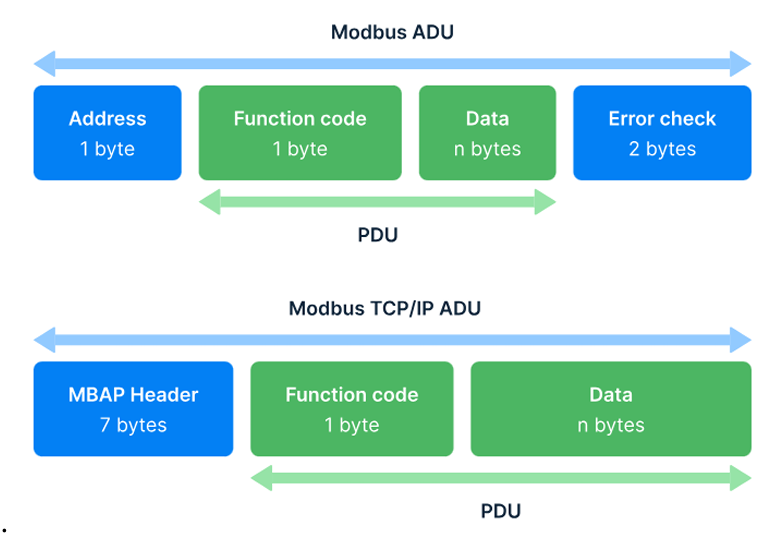
\includegraphics[width=0.8\columnwidth]{imgs/PDU and ADU.png}
    \caption[Short description for list of figures]{PDU and ADU}
    \label{fig-magnitude}
    \end{figure}%

    The Modbus communication structure consists of two main components: the communication layer and the physical layer. The most commonly used methods are Modbus ASCII, Modbus RTU and Modbus TCP/IP. In the physical layer, communication is provided via RS232, RS485, USB and CAN connections, while Ethernet is used in TCP/IP-based communications. The function code (1 byte) in the PDU (Protocol Data Unit) determines the operating mode of the devices, while the data field contains the request and response parameters between the master and slave devices.
    The Modbus message structure consists of the device address, function code, data field and error control mechanisms. The master device expects an immediate response to the commands it sends; if no response is received, it repeats the process and uses timing and error control mechanisms to ensure communication reliability. While Modbus allows flexible parameter configurations in some systems, fixed settings that cannot be changed by the user are used in other systems. Although Modbus is slower than other communication protocols, it is widely preferred in the industry due to its wide manufacturer support and flexible structure.
    



    \medskip

    \section{Energy Tracking}

    Energy monitoring systems are automation and control solutions developed to ensure effective control of energy consumption, increase energy efficiency and continuous monitoring of energy quality. These systems provide a wide data collection and evaluation infrastructure consisting of measurement devices, communication protocols and analysis software.
Energy monitoring systems ensure the healthy operation and management of production, transmission and distribution points in electrical facilities. These systems allow rapid detection and intervention of faults occurring in energy lines.
Energy monitoring systems perform critical functions in energy management and optimization processes. Thanks to the real-time monitoring feature, electrical parameters such as voltage, current, power and frequency are continuously monitored and analyzed.
In addition, remote control capability enables remote monitoring and control of energy systems via communication protocols. This feature provides ease of management, especially in energy systems spread over large areas. The energy efficiency and saving function allows the determination of unnecessary energy use and optimization of costs by analyzing consumption data. In addition, the harmonic and quality analysis feature of the system allows the detection of harmonics and other fluctuations that deteriorate energy quality. Thus, corrective measures are taken to improve energy quality and ensure system reliability. All these functions make energy monitoring systems an indispensable tool for modern energy management.



\begin{figure}[H]
    \centering
    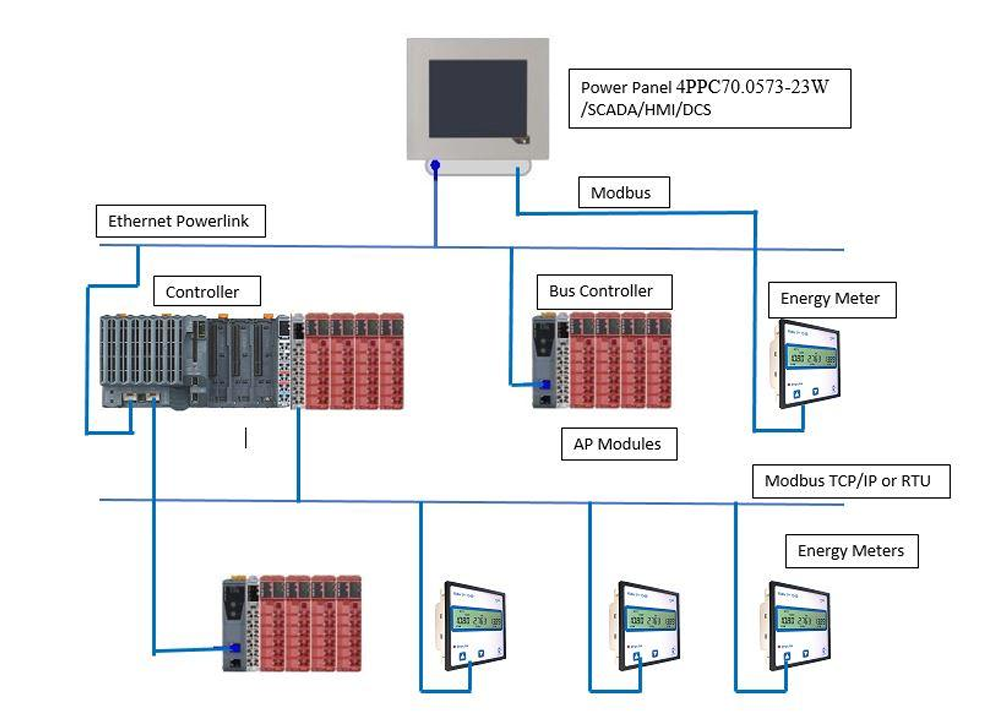
\includegraphics[width=0.8\columnwidth]{imgs/System Architecture of Energy Monitoring System.png}
    \caption[Short description for list of figures]{System Architecture of Energy Monitoring System }
    \label{fig-magnitude}
    \end{figure}%


    Energy monitoring systems are critical for monitoring energy consumption, increasing energy efficiency and ensuring energy quality. These systems help businesses reduce energy costs and provide sustainable energy management. Especially thanks to modern automation systems and communication technologies, energy monitoring systems have wider application areas.

    \medskip

    \subsection{Communication Protocols}  

    In energy monitoring systems, data transfer between devices is provided through communication protocols, and these protocols allow for secure, fast and uninterrupted data transmission. Modbus is the most widely used serial communication protocol in industrial automation systems. It provides a reliable communication infrastructure in energy monitoring systems by facilitating data transfer between devices such as PLCs and analyzers. The IEC 60870-5-101 protocol was specifically developed to ensure data security in critical energy infrastructures. It contributes to the continuous monitoring of energy systems by establishing secure communication between remote terminal units and smart electronic devices.


    \begin{figure}[H]
    \centering
    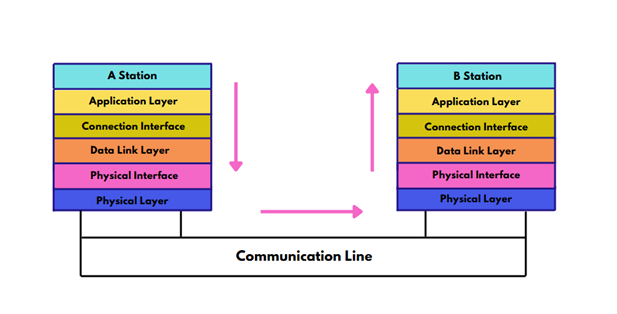
\includegraphics[width=0.8\columnwidth]{imgs/IEC 60870-5-101 Enhanced Performance Architecture Model.png}
    \caption[Short description for list of figures]{IEC 60870-5-101 Enhanced Performance Architecture Model }
    \label{fig-magnitude}
    \end{figure}%

    Wireless communication technologies such as ZigBee and Wi-Fi are frequently preferred in modern applications such as smart buildings and distributed energy production systems. These protocols have an important place in systems requiring wireless data transfer by offering low energy consumption and flexible connectivity. All these protocols provide uninterrupted data flow in energy monitoring systems, making energy management and analysis processes more reliable and efficient.



\medskip


\section{Modeling Motor}
This study aims to optimize energy consumption. The main energy-consuming components of the system are the conveyor systems and industrial robot arms in the production line. These two elements are directly connected to the drive systems, namely direct current (DC) motors, which convert electrical energy into mechanical energy in order to provide mechanical movement. Therefore, a large part of the total energy consumption is realized through these motors. In this context, a detailed examination of the operating characteristics of the motors in question and the regulation of their controllable parameters with the help of appropriate algorithms are of critical importance in terms of energy efficiency.

Within the scope of the project, the aim is to analyze the motor behavior by performing mathematical modeling of the DC motors used in the system.
The dynamic model of a typical DC motor is obtained by combining both electrical and mechanical subsystems.
In this context, in this project, we are trying to provide energy optimization by controlling these DC motors. The modeling of a DC motor is given below:

\begin{figure}[H]
    \centering
    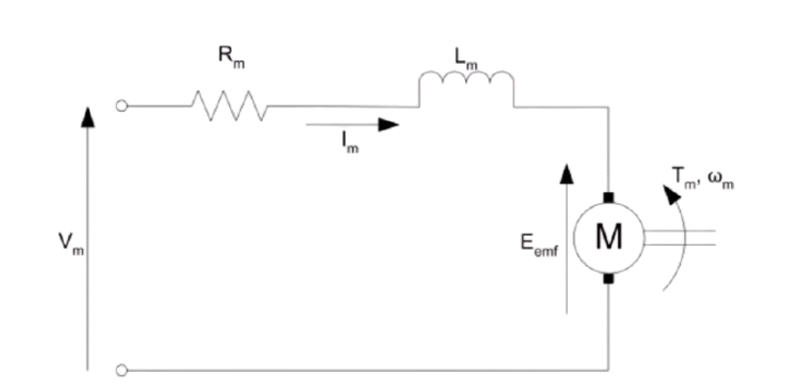
\includegraphics[width=0.8\columnwidth]{imgs/DC motor circuit.png}
    \caption[Short description for list of figures]{The circuit of DC motor }
    \label{fig-magnitude}
    \end{figure}%

    The stages of obtaining the transfer function of a DC electric motor are shown below:
    \begin{equation}
        V_m(t) = R_m I_m(t) + L_m \frac{d I_m(t)}{dt} + E_{emf} = 0
        \label{eq:dc_motor_voltage}
        \end{equation}

    The feedback voltage can be expressed as follows: 
        \begin{equation}
            E_{emf} = K_b W_m(t)
            \label{eqfeedback_voltage }
            \end{equation}

    The torque expression can be expressed as follows: 
            \begin{equation}
                T_m(t) = K_t I_m(t)
                \label{eq:torque_expression }
                \end{equation}

    The equivalent of torque in terms of viscosity and inertia is as follows:
            \begin{equation}
                T_m(t) = J_m \frac{d W_m(t)}{dt} + B_m W_m(t)
                \label{eq:mechanical_dynamics}
                \end{equation}
        

    Angular velocity equals the derivative of angular displacement:
            \begin{equation}
               W_m(t) = \frac{d \theta(t)}{dt}
                \label{eq:angular_velocity}
                \end{equation}
        

    If the voltage \( V_m(t) \) and torque \( T_m(t) \) expressed above are expressed in the frequency domain:
 
            \begin{equation}
                V_m(s) = R_m I_m(s) + L_m s I_m(s) + K_b W_m(s)
                \label{eq:voltage_laplace}
                \end{equation}
        
                \begin{equation}
                    T_m(s) = K_t I_m(s)
                    \label{eq:torque_current_laplace}
                    \end{equation}
                    
                \begin{equation}
                    T_m(s) = J_m s W_m(s) + B_m W_m(s)
                    \label{eq:mechanical_laplace}
                    \end{equation}
                        

    If \( K_t I_m(s) \) is substituted for the torque expression 

                \begin{equation}
                    K_t I_m(s) = J_m  W_m(s) + B_m W_m(s)
                    \label{eq:substituted_torque}
                    \end{equation}
        

    If the angular velocity is left alone, it is obtained as follows: 
    \begin{equation}
        W_m(s) = \frac{K_t I_m(s)}{J_m s + B_m}
        \label{eq:omega_from_current}
        \end{equation}
        
        If the angular velocity expression is substituted in equation 3.6, the voltage expression becomes 
        as follows: 

                \begin{equation}
                     V_m(s) = R_m I_m(s) + L_m s I_m(s) + K_b \left( \frac{K_t I_m(s)}{J_m s + B_m} \right)
                    \label{eq:vm_substitution_step1}
                    \end{equation}
        
                    \begin{equation}
                        V_m(s) = \left( R_m + L_m s + \frac{K_b K_t}{J_m s + B_m} \right) I_m(s)
                        \label{eq:vm_substitution_step2}
                        \end{equation}
    
    If the current expression is left alone, the following equation is obtained:

                \begin{equation}
                    I_m(s) = \frac{V_m(s)}{R_m + L_m s + \frac{K_b K_t}{J_m s + B_m}}
                    \label{eq:current_expression}
                    \end{equation}
        
    Earlier we stated that the angular velocity is:

    \begin{equation}
        W_m(s) = \frac{d \theta_m(s)}{ds}
        \label{eq:angular_velocity_laplace}
        \end{equation}
        
        Here the angular displacement, left alone, is equal to:
        
        \begin{equation}
            \theta_m(s) = \frac{W_m(s)}{s}
            \label{eq:angular_displacement_laplace}
            \end{equation}
            
            If the angular velocity is replaced by the expression in Equation 3.10 in the angle expression in 
Equation 3.15, the angular displacement is obtained as follows: 

\begin{equation}
    \theta_m(s) = \frac{K_t I_m(s)}{J_m s^2 + B_m s}
    \label{eq:theta_current_relation}
    \end{equation}

    
    If the expression for \( I_m(s) \) in Equation 3.16 is replaced by the expression for velocity in Equation 3.13, the angular displacement is equal to the following expression: 

\begin{equation}
    \theta_m(s) = 
    \frac{
    \left( \frac{K_t}{J_m s^2 + B_m s} \right) V_m(s)
    }{
    R_m + L_m s + \frac{K_b K_t}{J_m s + B_m}
    }
    \label{eq:theta_over_vm}
    \end{equation}

    Hence, with angular displacement \( \theta_m(s) \) as output and motor voltage \( V_m(s) \) as input, the 
transfer function is equal to the following expression: 

\begin{equation}
    \frac{\theta_m(s)}{V_m(s)} = 
    \frac{
    \frac{K_t}{J_m s^2 + B_m s}
    }{
    R_m + L_m s + \frac{K_b K_t}{J_m s + B_m}
    }
    \label{eq:transfer_unsimplified}
    \end{equation}

    
    \begin{equation}
        \frac{\theta_m(s)}{V_m(s)} = 
        \frac{K_t}{
        (s L_m + R_m)(s J_m + B_m) + K_b K_t
        }
        \label{eq:transfer_simplified}
        \end{equation}

        
    The efficiency \( \eta  \) of a DC motor is calculated by the following formulas: P is the motor power, \( P_{out}  \) is the output power of the motor, \( w \) is the angular speed: 

            \begin{equation}
    P_{\text{out}} = T_{\text{out}} \, \omega
    \label{eq:output_power}
    \end{equation}

    \begin{equation}
        \eta = \frac{P_{\text{out}}}{P} \cdot 100
        \label{eq:efficiency}
        \end{equation}
        

        \begin{figure}[H]
            \centering
            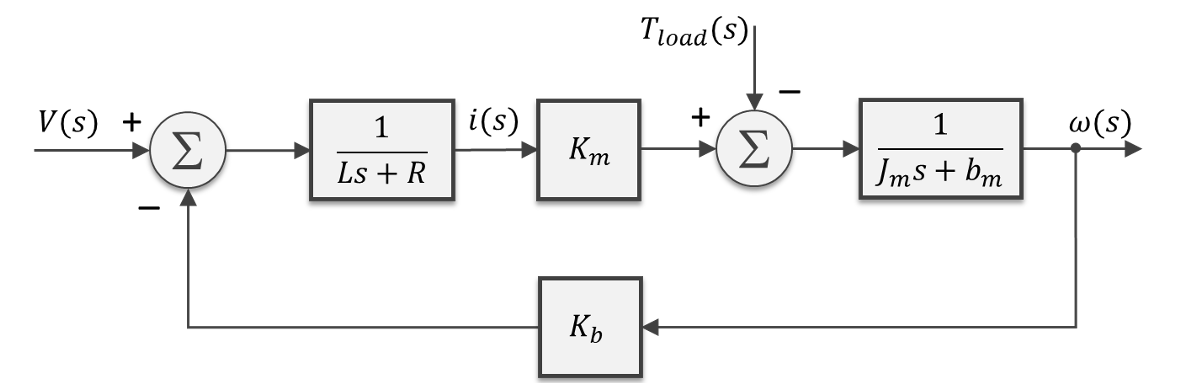
\includegraphics[width=0.8\columnwidth]{imgs/block diagram of the DC motor.png}
            \caption[Short description for list of figures]{The block diagram of the DC motor }
            \label{fig-magnitude}
            \end{figure}%

            Below is the Simulink drawing of the specified DC motor. In this model, terminal resistance, terminal inductance, back EMF constant, torque constant, rotor moment of inertia and mechanical friction coefficient specified as motor parameters in the data sheet are placed in the system. 5V is applied to the system as input voltage. In this structure; current, output voltage, output power, motor power, torque, motor speed, motor angle, load angle, load speed, counter torque and energy consumption are measured from the relevant points and collected via a 'bus selector' block and transferred to 'scope' blocks. Then, this data is connected to scope blocks and displayed graphically. Then, data is transferred to Matlab environment via 'to workspace' block; graphics are drawn here and added to the report.
            
    \begin{figure}[H]
        \centering
        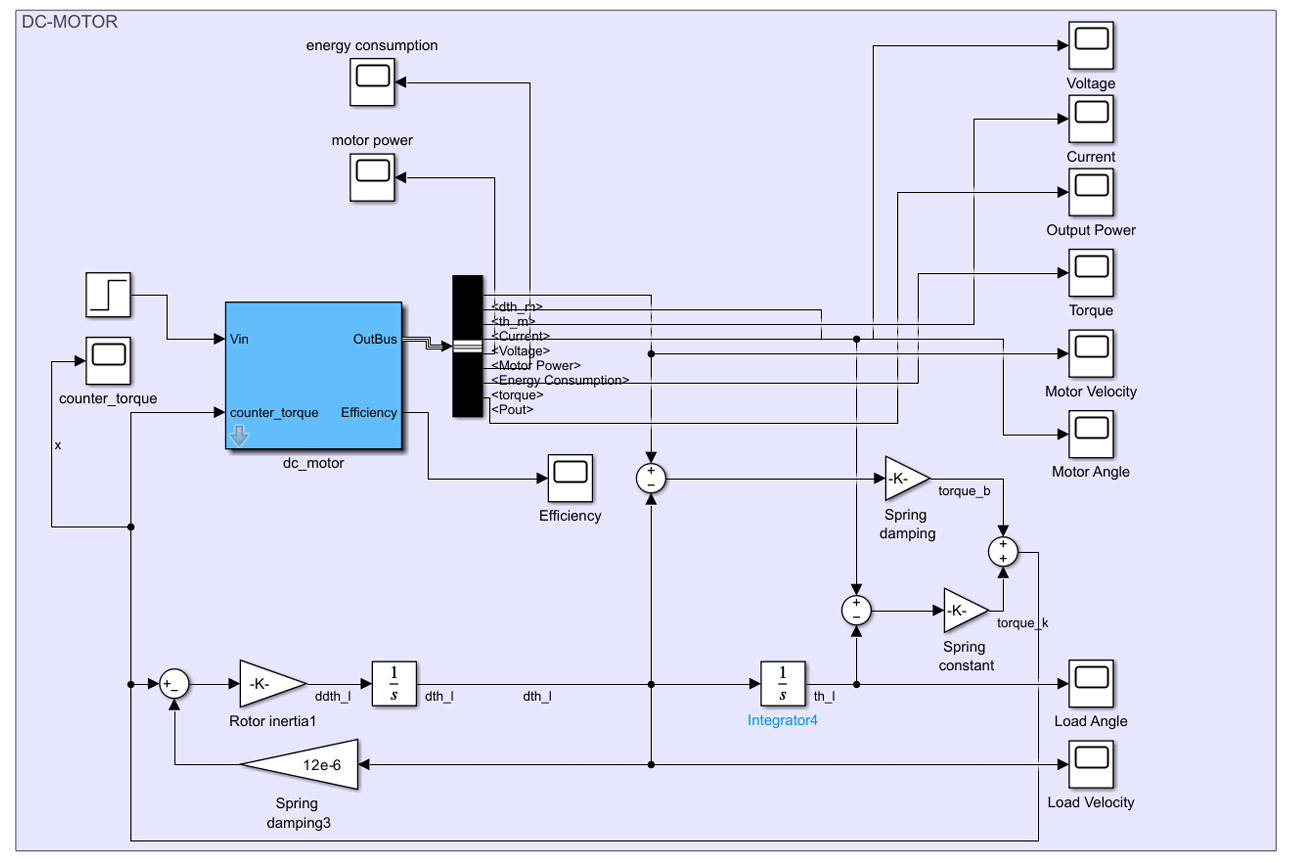
\includegraphics[width=0.8\columnwidth]{imgs/Simulink drawing of DC motor and load system.png}
        \caption[Short description for list of figures]{Simulink drawing of DC motor and load system }
        \label{fig-magnitude}
        \end{figure}%

        The internal structure of the subsystem (mask) block seen in blue above is as follows. Here, 
each parameter to be examined is connected to the outport port. 

\begin{figure}[H]
    \centering
    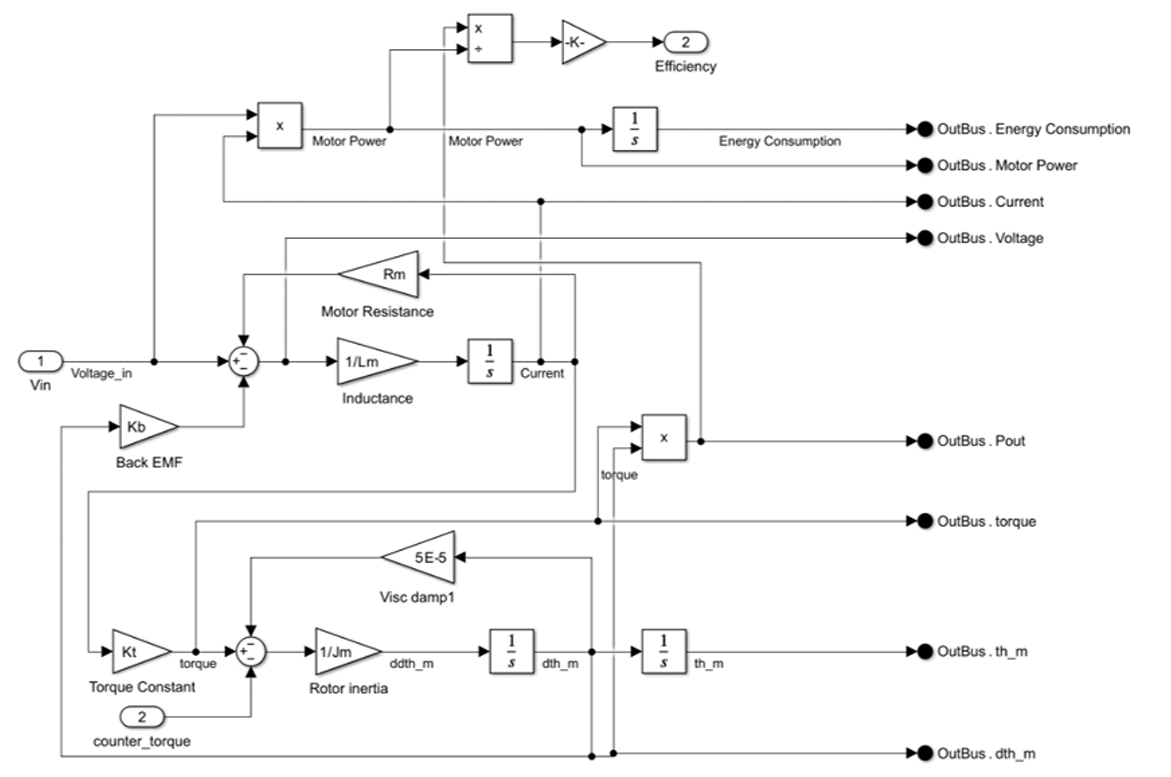
\includegraphics[width=0.8\columnwidth]{imgs/Tne inside of DC motor.png}
    \caption[Short description for list of figures]{Tne inside of DC motor }
    \label{fig-magnitude}
    \end{figure}%

    Detailed descriptions of the engine model and the corresponding graphical results are presented in Appendix B.

\section{dq Modeli} lÜç fazlı makine değişkenlerini (a-b-c) önce Clarke dönüşümü ile durağan $\alpha$–$\beta$ eksenlerine, ardından Park dönüşümü ile döner $d$–$q$ eksen takımına taşırız. $d$ ekseni rotor akısına paralel (\textit{akı bileşeni}), $q$ ekseni akıya dik (\textit{moment bileşeni}) olacak şekilde seçilirse akı ve moment birbirinden bağımsız kontrol edilebilir. Bu yapı asenkron motoru DC motor gibi kontrol etmeyi mümkün kılar \cite{macdonald1979dq,leonhard1996control}. dq modelinde motorun elektriksel dinamikleri, $d$ ve $q$ eksenlerine ait gerilim ve akım bileşenleri üzerinden ifade edilir. Bu eksen dönüşümü sayesinde, zamanla değişen üç fazlı sinyaller, sabit referans çerçevesinde iki bağımsız bileşen olarak kontrol edilir. Literatürde bu yöntem, \textit{Field Oriented Control} (FOC) gibi gelişmiş kontrol stratejilerinin temelini oluşturur \cite{blashke1972,sen1989}. Macdonald ve Sen'in \cite{macdonald1979dq} çalışmasında, dq modeli kullanılarak inverter–motor sisteminin kararlı çalışma noktaları belirlenmiş, akım kontrolü, kayma frekansı kontrolü ve akı kontrolü gibi stratejilerin kararlılık ve dinamik yanıt üzerindeki etkileri transfer fonksiyon analizi ile incelenmiştir. Elde edilen sonuçlar, akı ve momentin ayrık kontrolünün, sistemin hem düşük hem yüksek yük altında daha iyi performans gösterdiğini ortaya koymaktadır. \textbf{Standartlar ve Kısıtlar:} dq modelinin pratik uygulamalarında motor parametrelerinin doğru ölçülmesi kritik önemdedir. Bu ölçümler, IEC 60034-2-1 (verim ölçüm metotları), IEC 60034-4 (senkronizasyon metotları) ve IEC 60034-12 (başlatma metotları) gibi uluslararası standartlara uygun yapılmalıdır. Ayrıca, kayma frekansının aşırı yükselmesi akı zayıflamasına, düşük akım seviyelerinde ise belirli kontrol stratejilerinde kararlılık kaybına yol açabileceğinden kontrolcü tasarımında bu sınırlar dikkate alınmalıdır. \section{Clarke ve Park Dönüşümleri} Üç fazlı alternatif akım makinelerinin analizi ve kontrolünde, matematiksel ifadelerin basitleştirilmesi amacıyla \textbf{Clarke} ve \textbf{Park} dönüşümleri yaygın olarak kullanılmaktadır. Bu dönüşümler, motorun kontrol algoritmalarında zamanla değişen sinyallerin durağan veya döner referans sistemlerine aktarılmasını sağlar. Böylece, özellikle vektör kontrol (FOC) gibi yöntemlerde akı ve moment bileşenlerinin bağımsız kontrolü mümkün olur \cite{blashke1972,leonhard1996control}. \subsection{Clarke Dönüşümü (abc $\rightarrow$ $\alpha\beta0$)} Clarke dönüşümü, üç fazlı ($a$, $b$, $c$) dengeli sistemdeki akım veya gerilim bileşenlerini, durağan $\alpha$-$\beta$ eksen takımına ve sıfır bileşeni $i_0$’a dönüştürür. Bu sayede, üç fazlı sistem iki boyutlu Kartezyen koordinat sisteminde temsil edilir. $\alpha$ ekseni genellikle $a$ fazı ile aynı doğrultuda alınır, $\beta$ ekseni ise ona dik olarak tanımlanır. Dönüşüm matrisi aşağıda verilmiştir: \begin{equation} \begin{bmatrix} i_\alpha \\ i_\beta \\ i_0 \end{bmatrix} = \frac{2}{3} \begin{bmatrix} 1 & -\frac{1}{2} & -\frac{1}{2} \\ 0 & \frac{\sqrt{3}}{2} & -\frac{\sqrt{3}}{2} \\ \frac12 & \frac12 & \frac12 \end{bmatrix} \begin{bmatrix} i_a \\ i_b \\ i_c \end{bmatrix} \end{equation} Bu dönüşüm, IEC 60034 standardında tanımlı üç fazlı akım ölçümleri için uyumludur ve pratikte dijital kontrolörlerde hızlı hesaplama imkânı sunar. \subsection{Park Dönüşümü ($\alpha\beta$ $\rightarrow$ dq)} Park dönüşümü, Clarke dönüşümü ile elde edilen $\alpha$-$\beta$ durağan bileşenlerini, rotor akısına hizalanmış döner $d$-$q$ eksen takımına dönüştürür. Böylece, $d$ ekseni akı bileşenini, $q$ ekseni ise moment bileşenini temsil eder. $\theta$ açısı, rotor akı vektörünün $\alpha$ ekseni ile yaptığı açıdır ve genellikle enkoder, resolver veya sensörsüz gözlemciler ile belirlenir. \begin{equation} \begin{bmatrix} i_d \\ i_q \\ i_0 \end{bmatrix} = \frac{2}{3} \begin{bmatrix} \sin\theta & \sin\left(\theta-\frac{2\pi}{3}\right) & \sin\left(\theta+\frac{2\pi}{3}\right) \\ \cos\theta & \cos\left(\theta-\frac{2\pi}{3}\right) & \cos\left(\theta+\frac{2\pi}{3}\right) \\ \frac12 & \frac12 & \frac12 \end{bmatrix} \begin{bmatrix} i_a \\ i_b \\ i_c \end{bmatrix} \end{equation} Park dönüşümü, zamanla değişen sinyalleri sabit değerlere dönüştürdüğü için PI (Proportional–Integral) kontrolörlerin etkin şekilde çalışmasına olanak tanır. Bu, FOC algoritmalarında hassas tork ve akı kontrolü sağlamak için kritik öneme sahiptir. \textbf{Uygulama Notu:} Clarke ve Park dönüşümleri sayısal işlemcilerde (DSP, FPGA, mikrodenetleyici) gerçek zamanlı olarak hesaplanabilir. Ancak, $\theta$ açısının hatalı tahmini durumunda akı ve moment bileşenleri karışacağından kontrol performansı düşer. Bu nedenle, standartlara uygun hassas pozisyon/speed sensörleri veya yüksek doğruluklu sensörsüz tahmin yöntemleri kullanılmalıdır \cite{macdonald1979dq}. \section{3 Fazlı 4 kW 4 Kutuplu WEG Motor} Örnek motor: WEG W22 IE3, 4 kW, 4 kutup, 50 Hz \begin{itemize} \item Senkron hız: $1500$ d/dk \item Nominal hız: $\approx 1450$ d/dk \item Gerilim: 220–240/380–415 V ($\Delta$/Y) \item Koruma sınıfı: IP55 \item Soğutma: IC411-TEFC \end{itemize} \section{FOC (Field Oriented Control)} FOC, stator akımını akı ($d$) ve tork ($q$) bileşenlerine ayırıp, bu iki bileşeni PI akım çevrimleri ile referanslarında tutarak hızlı ve hassas moment/hız kontrolü sağlar. Temel fikir, rotor akı vektörünü $d$ eksenine sabitlemek ve $q$ eksenini moment üretimi için kullanmaktır. \section{Verimlilik Hesabı} Motor verimi: \begin{equation} \eta = \frac{P_{out}}{P_{in}} = \frac{T \cdot \omega}{P_{in}} \end{equation} \begin{itemize} \item \textbf{Doğrudan yöntem:} Giriş gücü (üç faz güç analizörü) ve çıkış gücü (torkmetre + devir) ölçülerek hesaplanır. \item \textbf{Dolaylı yöntem:} Bakır, demir, mekanik ve ek kayıplar ölçülerek toplam kayıp bulunur ve giriş gücünden düşülür. \end{itemize} Ölçüm ve raporlama IEC 60034-2-1 standardına uygun yapılmalıdır.
 
\medskip




\clearpage

\doublespacing % Do not change - required

\chapter{Implementation}
\label{ch4}

%%%%%%%%%%%%%%%%%%%%%%%%%%%%%%%%%%%%%%%
% IMPORTANT
\begin{spacing}{1} %THESE FOUR
\minitoc % LINES MUST APPEAR IN
\end{spacing} % EVERY
\thesisspacing % CHAPTER
% COPY THEM IN ANY NEW CHAPTER
%%%%%%%%%%%%%%%%%%%%%%%%%%%%%%%%%%%%%%%
\section{Discuss the practical realization of the proposed method}
In this section, practical implementation of smart energy monitoring and control system using Modbus protocol and Programmable Logic Controller (PLC) will be discussed. The system was designed to perform real-time data collection, analysis and control functions via a simulation program in order to increase energy efficiency and optimize energy consumption. The aim of the project is to monitor, optimize energy use in industrial facilities and reduce environmental impacts.

The basis of the system is to transfer energy data received from sensors to a PLC via Modbus protocol and process this data to optimize energy consumption. Here, a production system was implemented in Factory IO environment and then the PLC code suitable for this system was tried to be written via PLC software. PLC collects and processes data from sensors and will undertake the task of activating the control algorithm to improve the energy consumption of the system. It was decided to implement PID (Proportional-Integral-Derivative) as the control algorithm considered in this project. Both the simple and effective structure of the controller and its compatibility with PLC were effective in this decision. The purpose of using controllers is to turn devices on and off or adjust their speeds as necessary in order to minimize energy consumption and maximize system efficiency.
a
The simulation of the system in a virtual environment was performed with Factory IO software. This software has the ability to model and simulate industrial automation processes in a 3D environment and can be integrated with PLC and other automation systems. The simulation allowed the system to be tested in the real world and allowed the system to be evaluated without implementing a real application, considering the time and cost calculations.

The PLC used in the project process is the Siemens S7-1200 model. This model has high compatibility with the Modbus protocol and is widely used in industrial automation systems thanks to its fast processing capacity and expandable structure. In this project, a virtual PLC provided by Siemens, known as the PLCSIM application, was used instead of a real PLC. In the study, v18 versions were used in both programs. PLC Siemens S7-1200 was preferred due to the convenience of operating the PID control block and its compatibility with other programs.

The structure of the system components will be detailed below:

\textbf{Sensors:}: 

In order to control energy consumption, energy-related information such as speed, position, current of energy consuming system components must be known by the user. In this system, there are a number of power consuming components in the simulation environment. These are components such as conveyor systems that enable the movement of products in the system, robot arm that changes the position and state of the product. The robot arm transmits data to the PLC via the enerModbus protocol and fulfills the energy monitoring function by providing instant data for each energy parameter. 

\begin{figure}[H]
    \centering
    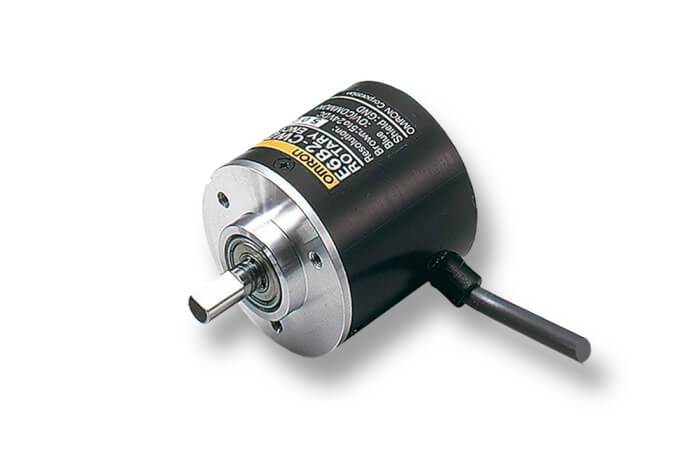
\includegraphics[width=0.8\columnwidth]{encoder.jpg}
    \caption[e6b2-c Encoder]{e6b2-c Encoder}
    \label{fig-magnitude}
\end{figure}%

\textbf{PLC (Programmable Logic Controller)}: 

A control device used in industrial automation systems. Siemens S7-1200 PLC is a widely used model in such systems and is known for its high performance. PLC usually communicates with sensors, actuators and other devices to control various processes. Such controllers analyze incoming data, apply certain logical operations and send output commands to make the system work more efficiently. One of the most important features of Siemens S7-1200 PLC is its compatibility with industrial protocols such as Modbus TCP/IP and Modbus RTU. These protocols allow PLC to exchange data with different devices and systems, thus ensuring seamless integration between devices.

\begin{figure}[H]
    \centering
    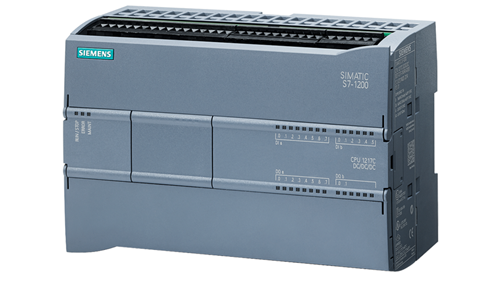
\includegraphics[width=0.8\columnwidth]{imgs/s7-1200.png}
    \caption[S7-1200 PLC]{S7-1200 PLC}
    \label{fig-magnitude}
\end{figure}%

\textbf{Communication Protocols:} 

Modbus is a communication protocol widely used in industrial automation systems. Designed to provide data transmission and communication between devices, this protocol allows data received from sensors to be processed securely and quickly, especially in PLC (Programmable Logic Controller) systems. There are different versions of Modbus; the most common of these are Modbus RTU (Remote Terminal Unit) and Modbus TCP/IP (Transmission Control Protocol/Internet Protocol).

In the Modbus RTU module, data is transmitted in digital format and communication is generally established over serial connections (such as RS-232, RS-485). This version is preferred in low-cost and simple systems because it has sufficient features in terms of speed and security. The RTU format provides error control and data verification mechanisms in each data frame, ensuring the security of data transmission.

Modbus TCP/IP, on the other hand, uses an Ethernet-based system and transmits data over the network using internet protocols. This version is preferred in larger systems, when a large number of devices need to be connected to each other. Modbus TCP/IP optimizes data communication in industrial automation systems by offering higher speeds and more device support.

\textbf{Control Algorithms}  

PID controller is a control system widely used in industrial automation and engineering applications, and includes Proportional (P), Integral (I), and Derivative (D) components. These components are combined to minimize the error between the target value and the current value of a system. PID controller is generally used to control temperature, speed, pressure, and other physical quantities. The basic components of PID control are explained below:

Proportional (P): The proportional component produces a control signal proportional to the error. The error is the difference between the target value and the actual value. This term determines the response speed of the system. A high Kp (proportional gain) value allows faster response to the error, but an excessively large Kp value may cause the system to be unstable.

Integral (I): The integral component takes into account the accumulation of the error over time. This term increases the error reset ability of the system and is used to eliminate static errors. However, a very large Ki (integral gain) value may cause the system to oscillate.

Derivative (D): The Derivative component takes into account the rate of change of the error. This term allows the system to reach equilibrium more smoothly and quickly. The value of Kd (derivative gain) helps to reduce the oscillations of the system, but a very high value of Kd can create excessive sensitivity in the system

\medskip

\section{Provide details on system architecture, hardware/software implementation}
\subsection{Software Programs}

Here, the software programs used in the project will be introduced first and their functions will be mentioned in the project. Then, hardware and software applications related to the system will be explained.

Many different software programs were used together in the system. What they are and their roles in the project are as follows:

\begin{itemize}
    \item \textbf{Matlab:} MATLAB (Matrix Laboratory), is a powerful software environment used for mathematical computations, data analysis, engineering and scientific research. Developed by MathWorks in the late 1980s, this software is widely used in many areas such as numerical computations, data analysis, graphics, simulations and algorithm development.

MATLAB is a matrix-based software environment, which is one of its most powerful features. While it focuses primarily on processing numerical data, it offers advanced mathematical functions, graphical tools, and a user-friendly programming language. MATLAB is often used in areas such as engineering calculations, control systems, signal processing, image processing, machine learning, and artificial intelligence.

MATLAB has a large number of built-in functions and toolboxes. Users can develop customized solutions in different application areas. For example, Simulink is a tool used with MATLAB for simulations of dynamic systems. It also allows users to visualize.

This project includes electric motors that drive the movement of robot arms and conveyors. Matlab was used to create models of these DC motors in the system and to relate the relationships of various physical quantities to each other and to energy.
\end{itemize}

\begin{itemize}
    \item \textbf{Tia Portal ve PLCSim:} TIA Portal (Totally Integrated Automation Portal) is a software platform developed by Siemens and provides integrated management of all components of industrial automation systems. This software allows users to program and monitor various devices such as PLC (Programmable Logic Controller), HMI (Human Machine Interface), motors, sensors. TIA Portal simplifies the software development, monitoring and maintenance processes of automation systems. Users can manage automation projects in an integrated manner through a single platform and accelerate the design process. This software is designed specifically for Siemens S7 PLCs and the Simatic product family and is widely used in production lines and industrial facilities.

    PLCSim is a simulation software that works integrated with Siemens' TIA Portal. This software allows PLC programs to be run in a virtual environment. PLCSim helps engineers verify their software by simulating software development and testing processes before using real hardware. This software is extremely useful in training and development processes, detecting programming errors and foreseeing the operation of automation systems.

    In this project, TIA Portal software was used to control the industrial production line simulation created in the Factory IO environment via a virtual PLC. This program written via the TIA portal was connected with the PLCSim selection from the drivers section in the Factory IO section and the inputs and outputs were matched and controlled. The program belonging to the project can be seen in detail in Appendix-1.
\end{itemize}

\begin{itemize}
    \item \textbf{Factory IO:} Factory IO is a simulation program used to model, test, and train industrial automation applications. Factory IO is used to perform simulations of PLC (Programmable Logic Controller) based systems, thus ensuring that industrial automation systems are designed and tested correctly.

    Factory IO includes devices such as a virtual production line, conveyor belts, robots, sensors, and actuators. These devices can be controlled with industrial protocols such as Modbus TCP/IP, allowing the user to test PLC programs without requiring real hardware. One of the biggest advantages of Factory IO is that it is compatible with industrial programming software such as TIA Portal or RSLogix 5000. This compatibility facilitates system integration and allows engineers to develop their software faster and more efficiently.

    Factory IO is used not only for simulation and training purposes, but also for the development of robotic systems, system design, and pre-application testing in the field. Users can simulate various industrial scenarios and applications in the software and increase the efficiency of the system by performing tests on these simulations. In addition, the software provides the necessary tools for users to test PLC programs, perform system verification, and perform performance analysis.
    
    As will be explained in detail in the following sections of this project, a simulation environment was created in the Factory IO environment where two parts will be combined. Then, the program was connected to the virtual PLC via PLCSim and the process was controlled from there.
\end{itemize}

\subsection{Created Project Environment}
This project includes a simulation program that involves producing two different parts that have key-lock compatibility with each other and then integrating them with a robot arm. As mentioned before, Factory IO, which produces a prototype of the real industrial world, was used as the simulation program. Figure 4.3 below shows the empty world of the Factory IO program.

\begin{figure}[H]
    \centering
    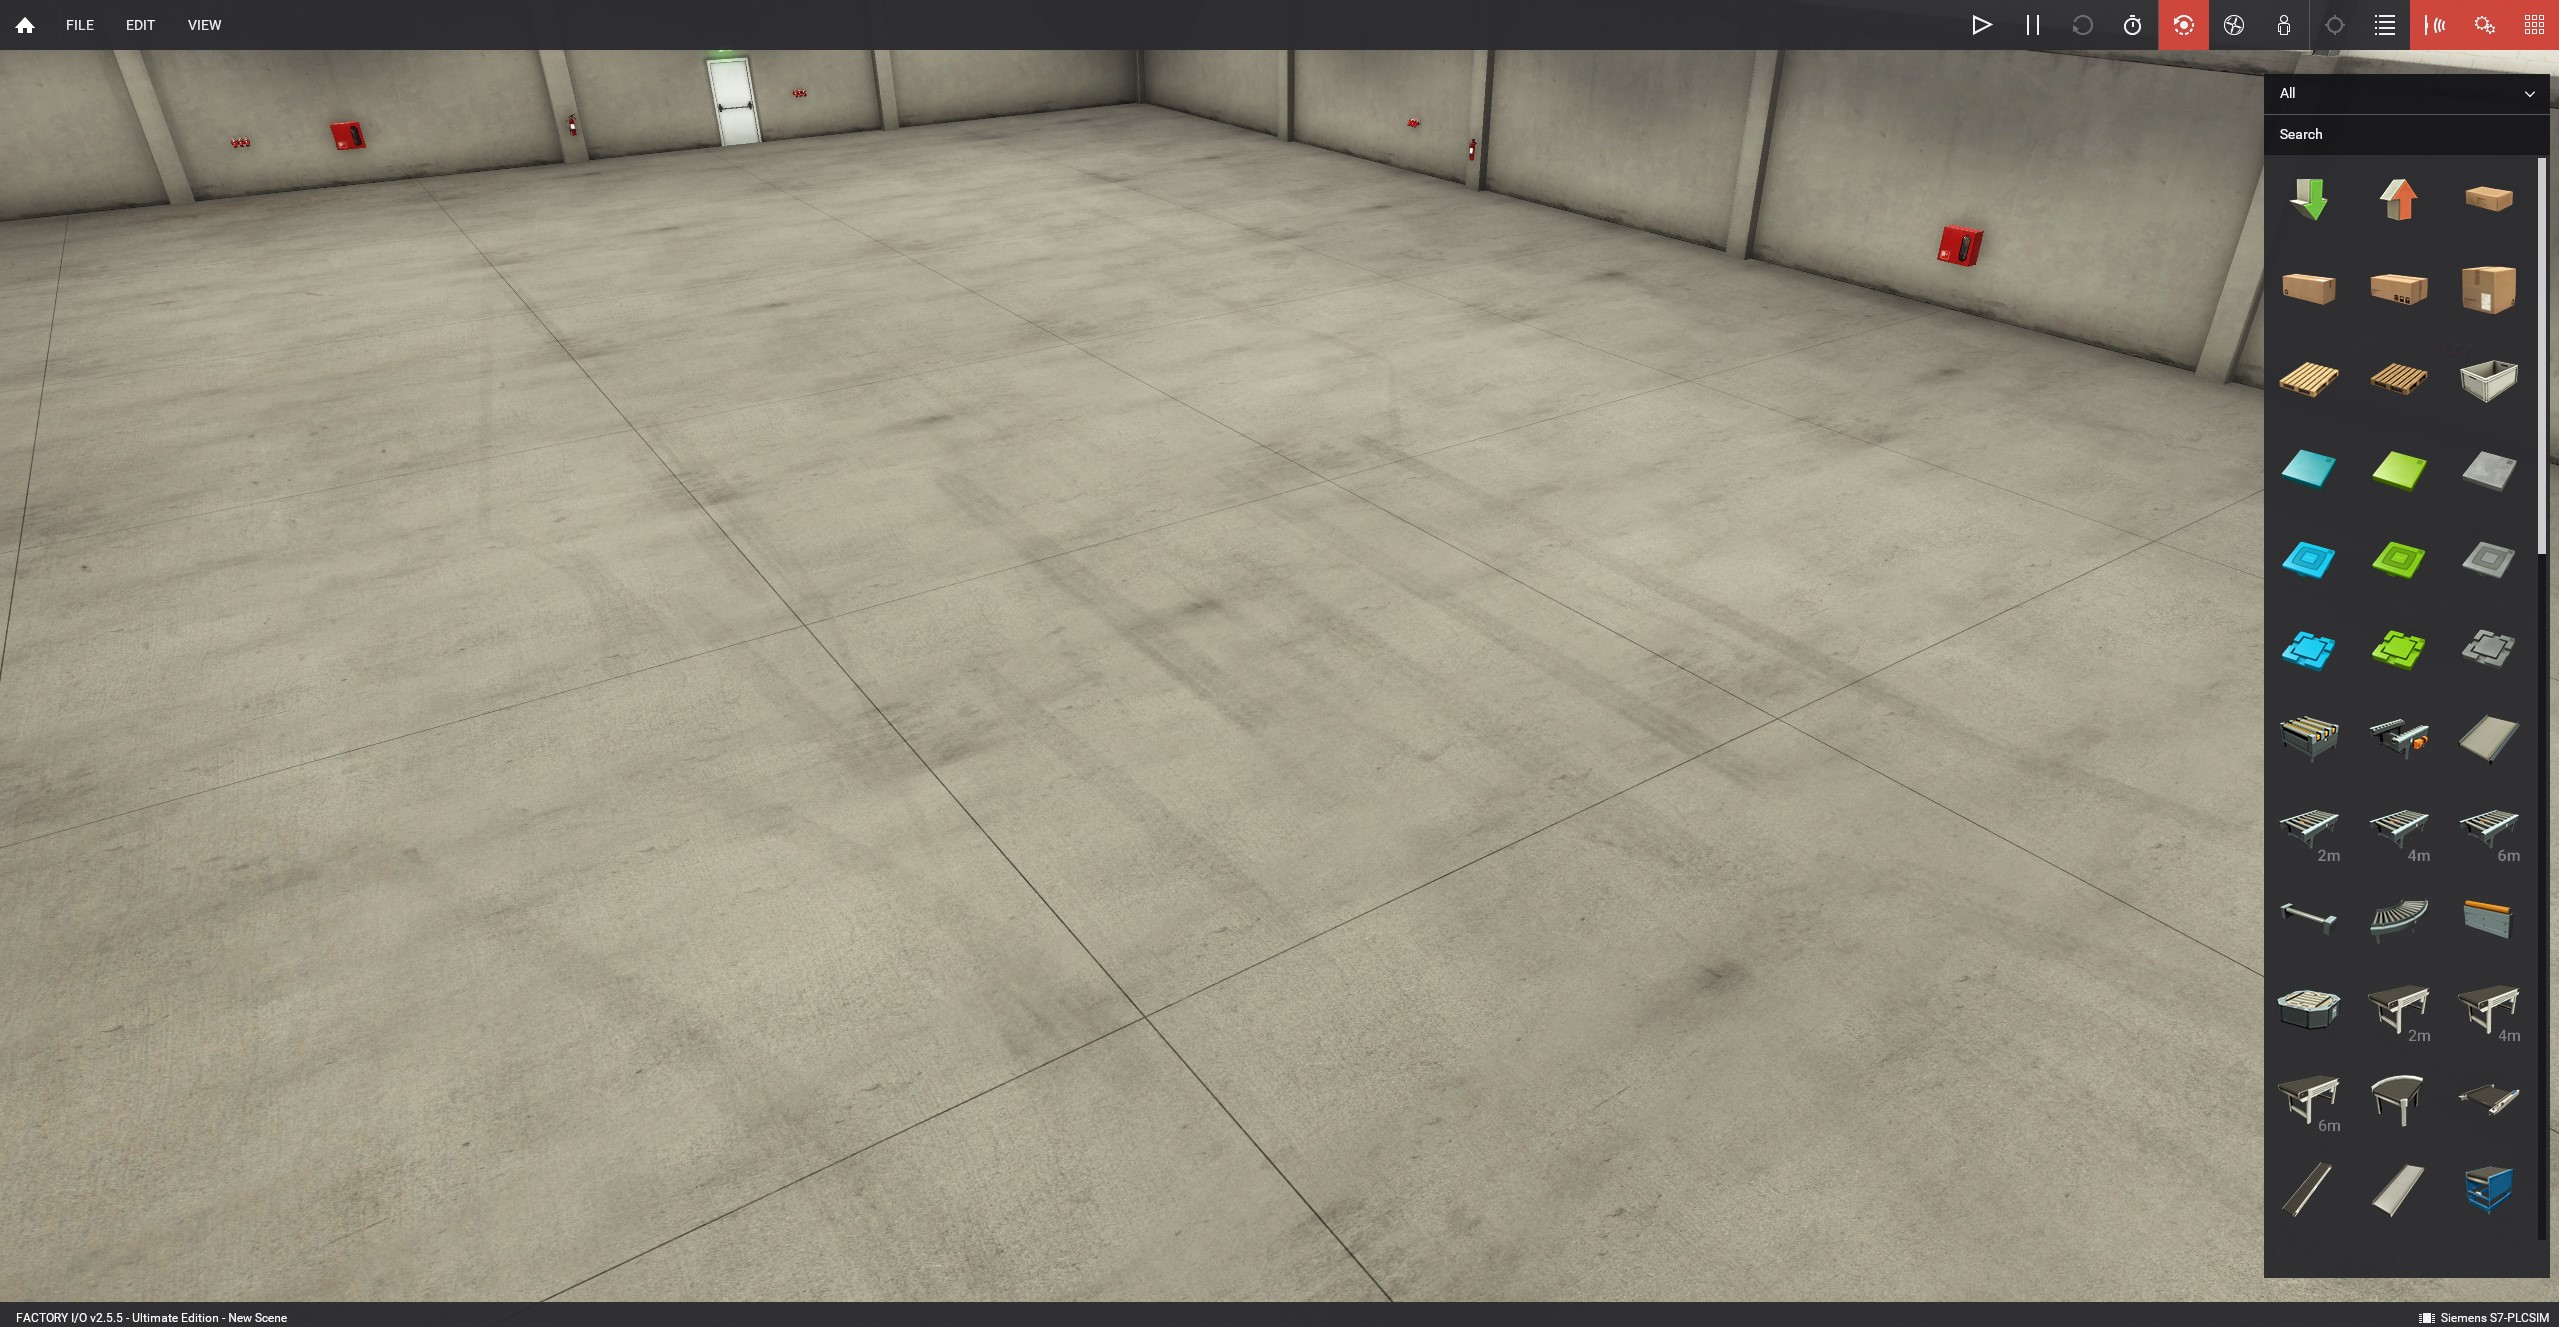
\includegraphics[width=0.5\columnwidth]{FactoryIO_baslangic_ortami.jpg}
    \caption[Factory IO starting environment]{Factory IO starting environment}
    \label{fig-magnitude}
\end{figure}%

As explained above, the project includes a simulation program that combines two parts. Below is a detailed examination of the system and an explanation of its working logic.

Below is the front view of the simulation system created in Figure 4.4.
\begin{figure}[H]
    \centering
    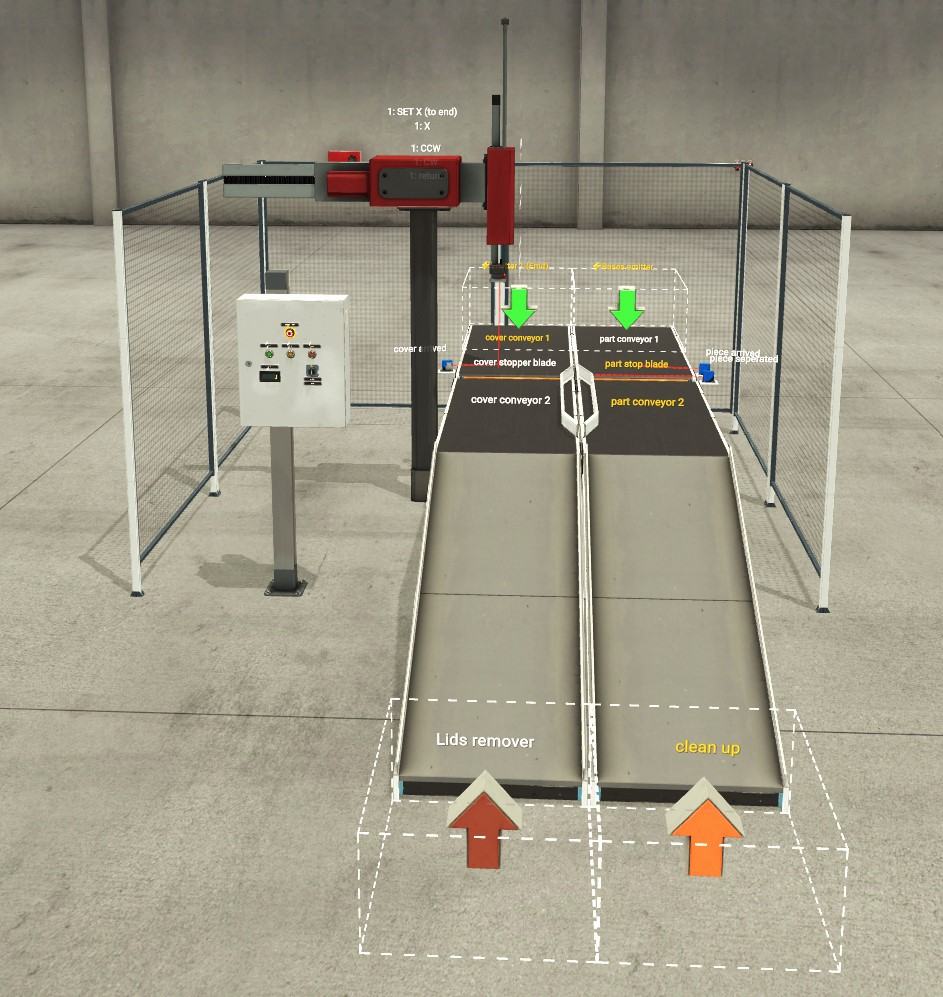
\includegraphics[width=0.5\columnwidth]{imgs/io/3.jpg}
    \caption[Front view of the created system]{Front view of the created system}
    \label{fig-magnitude}
\end{figure}%

The right view of the simulation system is shown in Figure 4.5.
\begin{figure}[H]
    \centering
    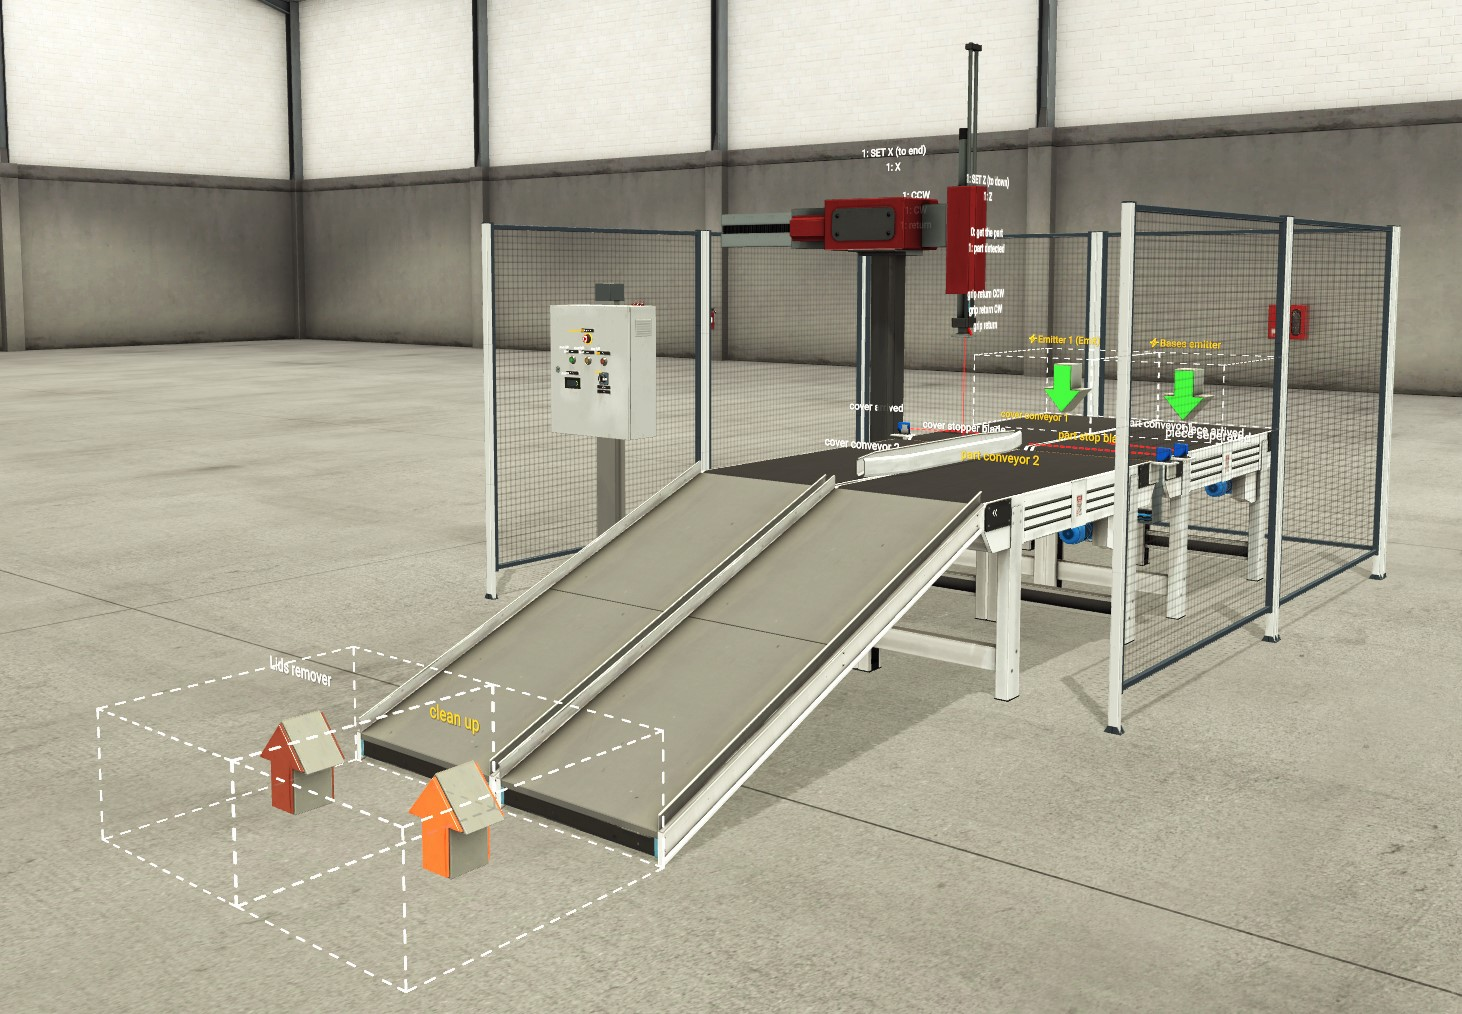
\includegraphics[width=0.5\columnwidth]{imgs/io/1.jpg}
    \caption[Right view of the created system]{Right view of the created system}
    \label{fig-magnitude}
\end{figure}%

The left view of the simulation system is shown in Figure 4.5.
\begin{figure}[H]
    \centering
    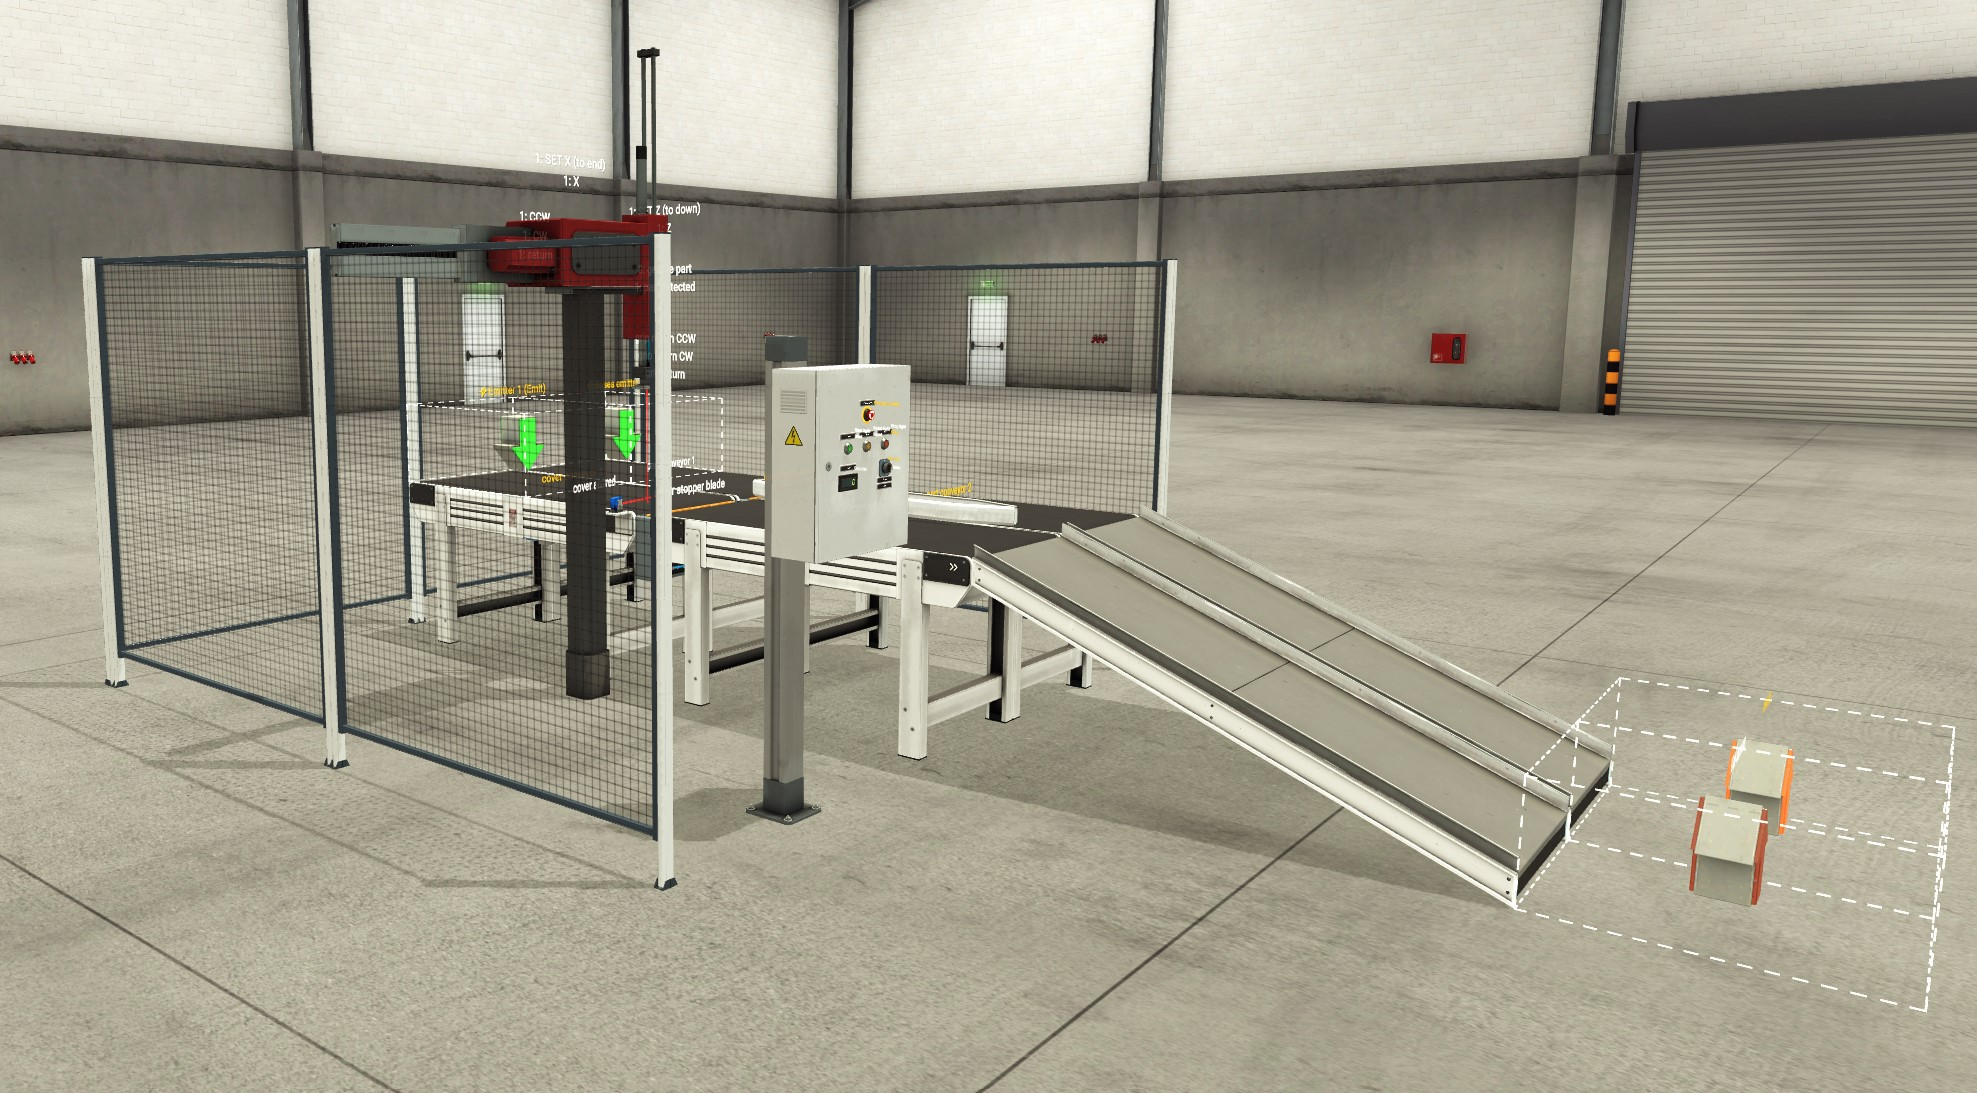
\includegraphics[width=0.5\columnwidth]{imgs/io/2.jpg}
    \caption[Left view of the created system]{Left view of the created system}
    \label{fig-magnitude}
\end{figure}%

\begin{itemize}
    \item \textbf{Working Principle of the System:} 
\end{itemize}

\begin{enumerate}
    \item \textbf{}\textbf{First stage:} When the start button is pressed while the emergency stop button shown in Figure 4.7 is closed, the part and cover conveyor shown in Figure 4.8 will start working.
    \item \textbf{} \textbf{Second stage:} When the created part and the cover are detected by the diffuse sensors seen in blue on both sides, the blades will lift up and the progress of the products on the belt will be stopped.
    \item \textbf{} \textbf{Third stage} The robot arm will come into play and, as seen in Figure 4.9, it will pick up the cover according to the values ​​set for it, place it on the body and drop it.
    \item \textbf{} \textbf{Fourth stage} After the parts are combined, the blade in front of the part will lift and the combined product will continue on the conveyor.
    \item \textbf{} \textbf{Fifth stage:} Finally, the product that has completed its movement on the conveyor will slide down from the platform and be removed as seen in Figure 4.11.
\end{enumerate}

\begin{figure}[H]
    \centering
    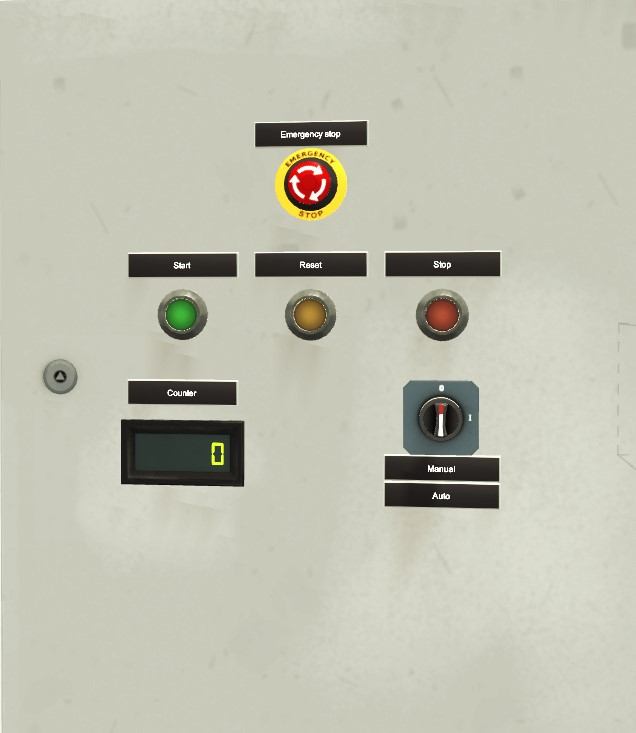
\includegraphics[width=0.65\columnwidth]{imgs/io/5.jpg}
    \caption[Board with buttons]{Board with buttons}
    \label{fig-magnitude}
\end{figure}%
\begin{figure}[H]
    \centering
    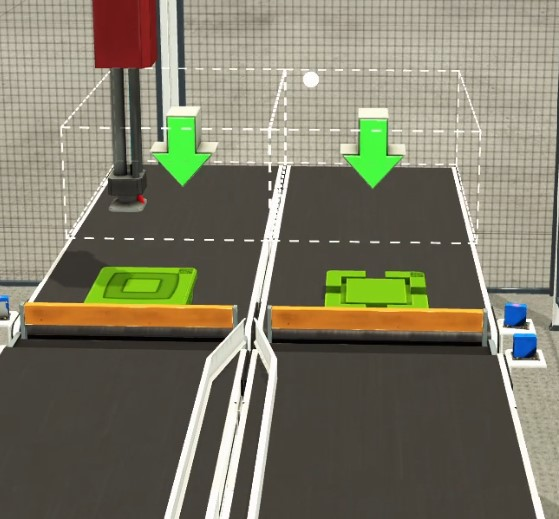
\includegraphics[width=0.65\columnwidth]{imgs/io/9.jpg}
    \caption[Creating parts and covers]{Creating parts and covers}
    \label{fig-magnitude}
\end{figure}%
\begin{figure}[H]
    \centering
    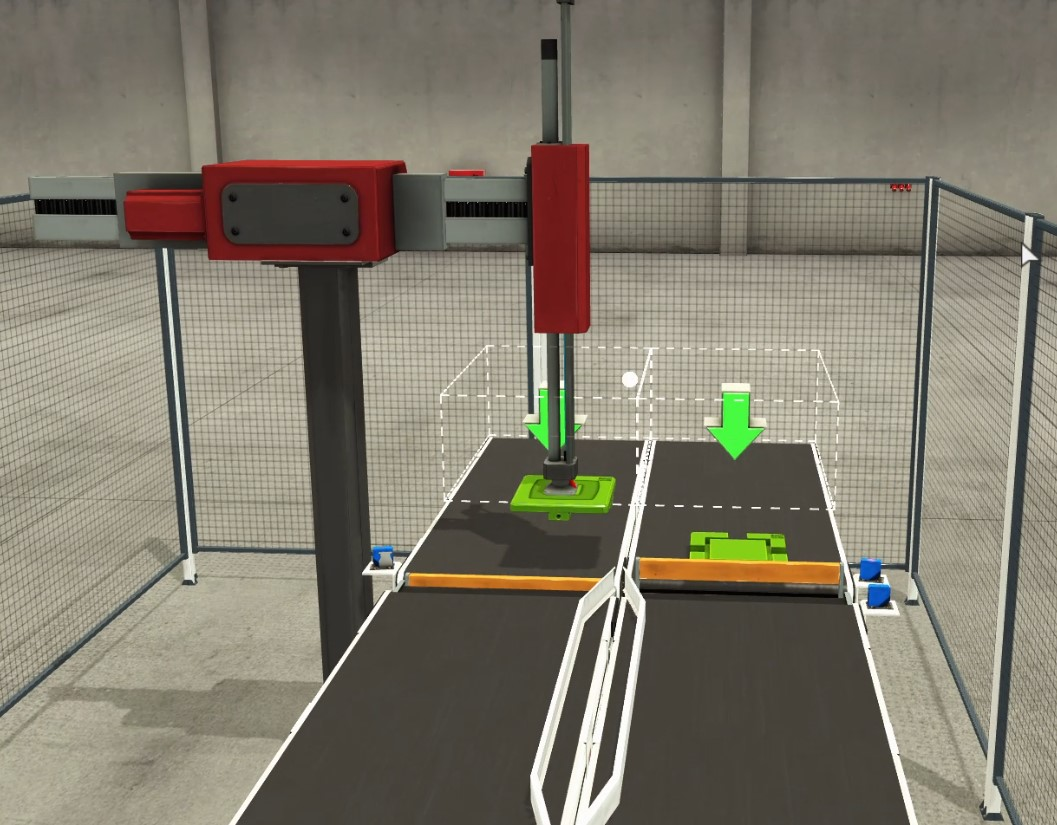
\includegraphics[width=0.8\columnwidth]{imgs/io/8.jpg}
    \caption[Robot arm moves the cover to the body]{Robot arm moves the cover to the body}
    \label{fig-magnitude}
\end{figure}%
\begin{figure}[H]
    \centering
    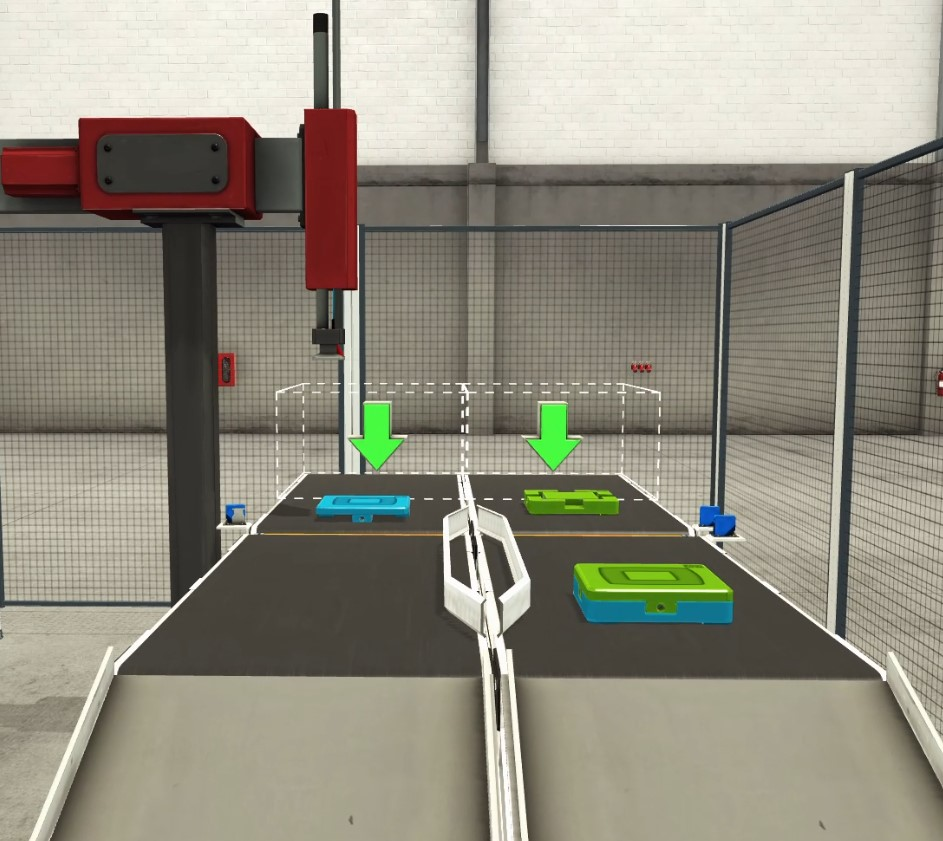
\includegraphics[width=0.8\columnwidth]{imgs/io/7.jpg}
    \caption[After the blades are opened, the produced part moves forward on the conveyor.]{After the blades are opened, the produced part moves forward on the conveyor.}
    \label{fig-magnitude}
\end{figure}%
\begin{figure}[H]
    \centering
    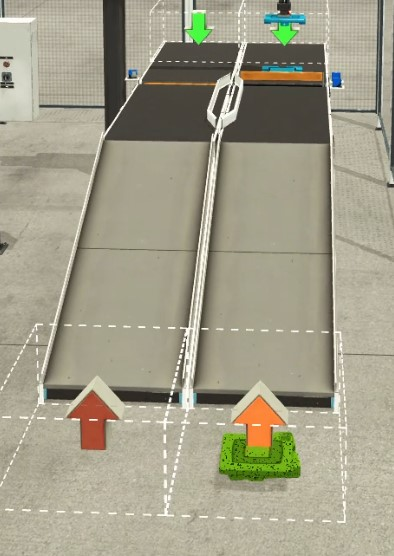
\includegraphics[width=0.5\columnwidth]{imgs/io/10.jpg}
    \caption[The manufactured part completes the conveyor and reaches the final stage.]{The manufactured part completes the conveyor and reaches the final stage.}
    \label{fig-magnitude}
\end{figure}%

All of these processes above are programmed via TIA Portal software and the inputs and outputs are placed in the same positions in the PLC and Factory IO software.
Below is the configuration of inputs and outputs in Factory IO according to PLCSim. The TIA Portal program that enables the operation of the system is presented in detail in Appendix-1.

\begin{figure}[H]
    \centering
    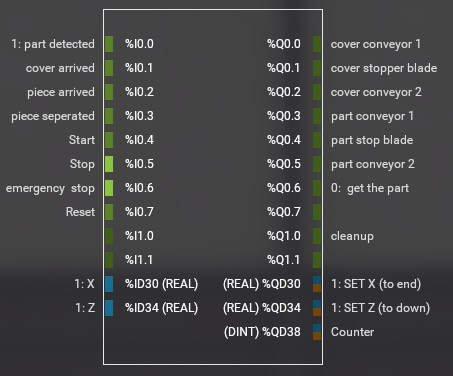
\includegraphics[width=0.5\columnwidth]{imgs/io/11.jpg}
    \caption[S7-1200 PLCSim driver settings]{S7-1200 PLCSim driver settings}
    \label{fig-magnitude}
\end{figure}%

\section{Highlight challenges and how they were addressed}
This project first includes the creation of an industrial production system in the Factory IO environment and the control of this system with a PLC. Then comes the determination and modeling of energy consumption parts. It is aimed to replace the parameters obtained from the industrial system and related to energy consumption in the model and operate with a PID controller at maximum efficiency.

In the part of the project so far, the system has been created, controlled with a PLC, energy consumption elements have been determined and energy-based modeled. The problem encountered is that the energy and parameters of the conveyors and robot arm located in the production facility and causing energy consumption cannot be obtained. The main problem causing this is that the Factory IO program does not have sensors such as an energy analyzer or encoder that will give the rotation speed of the motors directly. In addition, there is no data regarding the type of these motors or the simulation parameters. In other words, only the energy-related parameters of these two components need to be determined in order to complete the project. After this is done, the created model will be replaced and control will be provided with a PID controller. Research on this is ongoing.

Apart from this, while creating the system in Factory IO, a problem was encountered in which the system worked without pressing any buttons, and this was solved with the added emergency stop button. Apart from this, some minor system failures were experienced and easily solved.

In this study, it was aimed to transfer the energy data of the conveyor system to the PLC using the Factory I/O simulation software. However, as a result of the tests, it was not possible to transfer the data related to energy consumption directly to the PLC in the simulation environment at the expected level. Due to these technical limitations experienced during the implementation process, it was decided to evaluate the possibility of continuing with the SCADA (Supervisory Control and Data Acquisition) system, which offers a more stable and measurable structure in the monitoring and control component of the project.

SCADA systems provide high-level visualization, data collection and central control in industrial automation and energy monitoring projects; enabling real-time process monitoring. In this context, parameters such as the operating status of the conveyor system modeled in the Factory I/O environment, the triggering time of the motors, and the active times of the loads in the system can be digitized via the PLC and transferred to the SCADA screen. By using a Ladder diagram to be developed within the PLC, the operating times of the motors can be measured with counters or timers (TON blocks) and the approximate energy consumption can be calculated based on these values. For example, a certain fixed power factor is defined for each motor and the energy consumption data is obtained by multiplying it by the motor operating time. When this data is transferred to the SCADA system, both instantaneous energy consumption and total cumulative consumption can be monitored graphically via the user interface. In addition, thanks to the alarm and reporting features of SCADA; automatic warning systems can be created for situations such as exceeding energy limit values ​​and periodic consumption analyses can be reported. Thus, a realistic and traceable energy management system can be established in the light of the data obtained from the processes created in the simulation environment without using a physical energy analyzer in the field. This approach allows students to develop both PLC programming and SCADA application development competencies in an integrated manner.

\medskip

\clearpage
\doublespacing % Do not change - required

\chapter{Simulations, Results and Discussion}
\label{ch5}

%%%%%%%%%%%%%%%%%%%%%%%%%%%%%%%%%%%%%%%
% IMPORTANT
\begin{spacing}{1} %THESE FOUR
\minitoc % LINES MUST APPEAR IN
\end{spacing} % EVERY
\thesisspacing % CHAPTER
% COPY THEM IN ANY NEW CHAPTER
%%%%%%%%%%%%%%%%%%%%%%%%%%%%%%%%%%%%%%%

\section{Present experimental results, data analysis, and performance evaluation}
As mentioned before, the system is designed and simulated in the Factory IO environment. Since the program is a simulation of a factory environment, it cannot be expected to be fully compatible with the real world. Due to modeling errors and simulation errors, the system cannot be expected to work at an optimal level.

A part and cover clamping project coded with PLC and implemented in the simulation environment works successfully in the simulation. From time to time, due to programmatic errors or sensor detection programs, it has been observed that although the parts are programmed to be the same size and their midpoints overlap, the midpoints do not overlap and different parts are clamped.

It has been determined that the encoders planned to be used for the determination of energy-related quantities such as speed and position of the system are not available in the simulation environment. The main reason here is thought to be that the program cannot reach the high-frequency data processing capacity of the encoders. At this point, the possibility of slowing down the system speed and programming a manual encoder or using a different tool for simulation is considered in future studies.

After the energy-related components of the motors are obtained, it is thought that the simulation can be performed by replacing the parameters in the currently ready DC motor model. Then, it is thought that a PID block design will be made in the Matlab software with the obtained data and then the coefficients found will be transferred to the program with the PID block in the PLC.

In this way, the optimization of the system's energy saving will be provided by working together with many programs on energy-consuming motors.
\medskip

\section{Compare results with existing approaches}
In our study, the system architecture is based on a PLC-based structure, and energy consumption is monitored in real time; data processing is performed with PLC and a virtual modeling of physical systems is provided using Factory IO software. In this structure, control and monitoring operations are carried out directly through the interaction between PLC and Factory IO. Within the scope of the software platform, PID control applications are implemented for users and data visualization is provided. In the "Development of a Real-Time Energy Monitoring Platform" study, data is received from the energy analyzer using the RS485 communication protocol and a basic level graphical data monitoring service is offered to the user via an interface developed with the DELPHI language; there is no virtual modeling or simulation integration in this project. In the "Industrial IoT-Based Energy Monitoring System Using Data Processing at Edge" study, the system architecture is based on the edge computing approach, data is collected on a local server and analyzed via a JavaScript-based data processing engine and presented to the user with an advanced dashboard interface; in addition, automatic e-mail notification mechanisms are also included in the system. However, there is no simulation or modeling infrastructure representing the physical process in this study. In this context, although the studies examined aim to monitor energy, they show significant differences in terms of system architectures, data processing methods and software platforms.
\medskip

\section{Discuss key findings and their implications}
The important negative finding, as mentioned before, is the difficulty in transferring data to the PLC due to the encoder problem in the simulation program. Although other processes were ready, the energy-based control of the system could not be performed due to this problem.

The important positive findings are that industrial processes can be successfully performed in the simulation environment. Conversely, it is highly probable that the processes implemented in the simulation environment can also be performed in the real world. If this is done, sensor problems can also be prevented.
\medskip

\clearpage
\doublespacing % Do not change - required

\chapter{Conclusion and Future Work}
\label{ch6}

%%%%%%%%%%%%%%%%%%%%%%%%%%%%%%%%%%%%%%%
% IMPORTANT
\begin{spacing}{1} %THESE FOUR
\minitoc % LINES MUST APPEAR IN
\end{spacing} % EVERY
\thesisspacing % CHAPTER
% COPY THEM IN ANY NEW CHAPTER
%%%%%%%%%%%%%%%%%%%%%%%%%%%%%%%%%%%%%%%



    \section{Main Contributions of the Study}

Within the scope of this project, a real-time energy monitoring and control system integrated with a PLC using a Modbus-based communication protocol was developed. The modular architecture of the system allows for future expansion and improvement work. In addition, the design of the system using low-cost hardware that complies with industrial standards provided both economic efficiency and ease of application.
    \medskip

    \section{Limitations of The Work}

The system developed within the scope of the project was limited to a specific PLC model and energy analyzer. The integration of the system with different brands and models of devices was not tested. In addition, the communication infrastructure was implemented only via the Modbus RTU protocol, and compatibility with other communication protocols (such as Modbus TCP/IP or OPC UA) was not evaluated. Real-time performance analysis was performed only on specific sample load scenarios.    
    \medskip

    \section{Suggestions for Future Studies}

In future studies, the system can be integrated with different communication protocols to increase its flexibility. In addition, more in-depth analysis of energy consumption data can be made possible by adding advanced data analytics algorithms. Redesigning the system to work on different hardware platforms and integrating it with cloud-based monitoring systems will also enable the project outputs to be transferred to wider areas of use.
    \medskip




\clearpage

%\doublespacing % Do not change - required

\chapter{How To ...... in\LaTeX ?}
\label{chHT}

%%%%%%%%%%%%%%%%%%%%%%%%%%%%%%%%%%%%%%%
% IMPORTANT
\begin{spacing}{1} %THESE FOUR
\minitoc % LINES MUST APPEAR IN
\end{spacing} % EVERY
\thesisspacing % CHAPTER
% COPY THEM IN ANY NEW CHAPTER
%%%%%%%%%%%%%%%%%%%%%%%%%%%%%%%%%%%%%%%

{\color{red}This section provides detailed examples of equations, tables, figures, etc. that you will use in LATEX to help you with your interim and final reports. Please review the recommended websites!!!!!!!}

\section{Introduction}

In this section, some crucial point about how to fill this template are given such as formulation, figures, tables etc.

\section{How to define an equation ?}
\medskip
A simple and a complex examples are given in equation (\ref{eq:simpleexample}) and equation (\ref{eq:complexexample})

\begin{equation}
    u(t) = K_p e \left( t\right) + K_i \int_0^t \left( \tau\right) dt + K_d \frac{d e \left( t\right)}{dt}
    \label{eq:simpleexample}
\end{equation}

%
%
\begin{equation}
\begin{split}
& \mathbf{F_1}=\{i \ | \ |\beta_i|=Z, |G\left(\mathbf{x_i}\right)|\geq \epsilon \} \\
& \mathbf{F_2}=\{i \ | \ 0< |\alpha_i|<P, |G_2\left(\mathbf{x_{ijkl}}\right)|=0  \} \\ 
& \mathbf{\omega_{PSA}}=\{k \ | \ |\lambda_i|=0, | \phi\left(\mathbf{x_i}\right)|\leq \varepsilon  \}
\end{split}
\label{eq:complexexample}
\end{equation}
%
%
For more detailed informations, you can use \url{https://www.overleaf.com/learn/latex/Mathematical_expressions} and "Further reading" sections given in previous website.
%
%
\subsection{How to define matrix?}


\begin{equation}
\boldsymbol{\Omega}=\begin{bmatrix}
	\Omega_{s_0}\\
	\Omega_{s_1}\\
	\vdots\\
	\Omega_{s_k}
	\end{bmatrix} =-\mathbf{\Theta}\begin{bmatrix}
	1\\
	2\\
	\vdots\\
	K
	\end{bmatrix} \ , \
	\label{eq:10}
\end{equation}


\begin{equation}
%\begin{split}
\boldsymbol{\Omega}=\begin{bmatrix}
	\Omega_{s_0}\\
	\Omega_{s_1}\\
	\vdots\\
	\Omega_{s_k}
	\end{bmatrix} =-\mathbf{\theta}\begin{bmatrix}
	1\\
	2\\
	\vdots\\
	K
	\end{bmatrix} \ , \
    	\mathbf{\theta}=\begin{bmatrix}
	\theta_{11} & \theta_{12} & \cdots &\theta_{1k} \\
	\theta_{21} & \theta_{22} & \cdots &\theta_{2k} \\
	\vdots & \vdots & \ddots & \vdots \\
    \theta_{k1} & \theta_{k2} & \cdots &\theta_{kk}
	\end{bmatrix}^{-1}
%\end{split}        
	\label{eq:10}
\end{equation}
%
%






\subsection{How to split Long equations?}

You can use "split" command given as below:

\begin{equation}
\begin{split}
&\boldsymbol{\Omega}=\begin{bmatrix}
	\Omega_{s_0}\\
	\Omega_{s_1}\\
	\vdots\\
	\Omega_{s_k}
	\end{bmatrix} =-\mathbf{\theta}\begin{bmatrix}
	1\\
	2\\
	\vdots\\
	K
	\end{bmatrix} \ , \\
    &
    	\mathbf{\theta}=\begin{bmatrix}
	\theta_{11} & \theta_{12} & \cdots &\theta_{1k} \\
	\theta_{21} & \theta_{22} & \cdots &\theta_{2k} \\
	\vdots & \vdots & \ddots & \vdots \\
    \theta_{k1} & \theta_{k2} & \cdots &\theta_{kk}
	\end{bmatrix}^{-1}
\end{split}        
	\label{eq:10}
\end{equation}

%
%
For detailed information you can use the following website.

\medskip
For detailed information you can use the following website.\\
\url{https://www.overleaf.com/learn/latex/Aligning_equations_with_amsmath}


\subsection{Significant Greek Symbols utilized in \LaTeX}

Some symbols are given below



In addition to these, you can find much more detailed information on the website below. In addition, LLM structures will be very helpful.

\begin{itemize}
\item \url{https://www.overleaf.com/learn/latex/List_of_Greek_letters_and_math_symbols}
\item \url{https://ftp.cc.uoc.gr/mirrors/CTAN/info/symbols/comprehensive/symbols-a4.pdf}
\item \url{https://www.geeksforgeeks.org/greek-alphabet-symbols/}

\item Your LLM Friends(ChatGPT, Deepseek etc) 
\end{itemize}


\subsubsection{Greek Alphabet}
\subsubsection{Lowercase Letters}
\begin{tabular}{ll | ll | ll}
\textbackslash alpha & $\alpha$ & \textbackslash nu & $\nu$ & \textbackslash upsilon & $\upsilon$ \\
\textbackslash beta & $\beta$ & \textbackslash xi & $\xi$ & \textbackslash phi & $\phi$ \\
\textbackslash gamma & $\gamma$ & \textbackslash omicron & $o$ & \textbackslash chi & $\chi$ \\
\textbackslash delta & $\delta$ & \textbackslash pi & $\pi$ & \textbackslash psi & $\psi$ \\
\textbackslash epsilon & $\epsilon$ & \textbackslash rho & $\rho$ & \textbackslash omega & $\omega$ \\
\textbackslash zeta & $\zeta$ & \textbackslash sigma & $\sigma$ &  &  \\
\textbackslash eta & $\eta$ & \textbackslash tau & $\tau$ &  &  \\
\textbackslash theta & $\theta$ & \textbackslash iota & $\iota$ &  &  \\
\end{tabular}

\subsubsection{Uppercase Letters}
\begin{tabular}{ll | ll | ll}
\textbackslash Gamma & $\Gamma$ & \textbackslash Lambda & $\Lambda$ & \textbackslash Sigma & $\Sigma$ \\
\textbackslash Delta & $\Delta$ & \textbackslash Xi & $\Xi$ & \textbackslash Upsilon & $\Upsilon$ \\
\textbackslash Theta & $\Theta$ & \textbackslash Pi & $\Pi$ & \textbackslash Phi & $\Phi$ \\
\textbackslash Omega & $\Omega$ & \textbackslash Psi & $\Psi$ &  &  \\
\end{tabular}

\subsubsection{Mathematical Symbols}
\subsubsection{Commonly Used Symbols}
\begin{tabular}{ll | ll | ll}
\textbackslash infty & $\infty$ & \textbackslash pm & $\pm$ & \textbackslash times & $\times$ \\
\textbackslash sum & $\sum$ & \textbackslash prod & $\prod$ & \textbackslash int & $\int$ \\
\textbackslash sqrt & $\sqrt{x}$ & \textbackslash frac & $\frac{a}{b}$ & \textbackslash lim & $\lim$ \\
\textbackslash sin & $\sin x$ & \textbackslash cos & $\cos x$ & \textbackslash tan & $\tan x$ \\
\textbackslash log & $\log x$ & \textbackslash exp & $\exp x$ & \textbackslash ln & $\ln x$ \\
\end{tabular}

\subsubsection{Relational Symbols}
\begin{tabular}{ll | ll | ll}
\textbackslash leq & $\leq$ & \textbackslash geq & $\geq$ & \textbackslash neq & $\neq$ \\
\textbackslash approx & $\approx$ & \textbackslash equiv & $\equiv$ & \textbackslash subset & $\subset$ \\
\textbackslash supset & $\supset$ & \textbackslash subseteq & $\subseteq$ & \textbackslash supseteq & $\supseteq$ \\
\end{tabular}

\subsubsection{Logic and Set Notation}
\begin{tabular}{ll | ll | ll}
\textbackslash forall & $\forall$ & \textbackslash exists & $\exists$ & \textbackslash neg & $\neg$ \\
\textbackslash in & $\in$ & \textbackslash notin & $\notin$ & \textbackslash emptyset & $\emptyset$ \\
\textbackslash cap & $\cap$ & \textbackslash cup & $\cup$ & \textbackslash subseteq & $\subseteq$ \\
\textbackslash wedge & $\wedge$ & \textbackslash vee & $\vee$ & \textbackslash Rightarrow & $\Rightarrow$ \\
\textbackslash Leftrightarrow & $\Leftrightarrow$ & \textbackslash bot & $\bot$ & \textbackslash top & $\top$ \\
\end{tabular}

\subsubsection{Brackets and Parentheses in Mathematical Expressions}
The following web site will help you for detailed information about Brackets and Parentheses " 
\url{https://www.overleaf.com/learn/latex/Brackets_and_Parentheses} " .




















\section{How to upload Figure etc?}


\begin{figure}
\centering
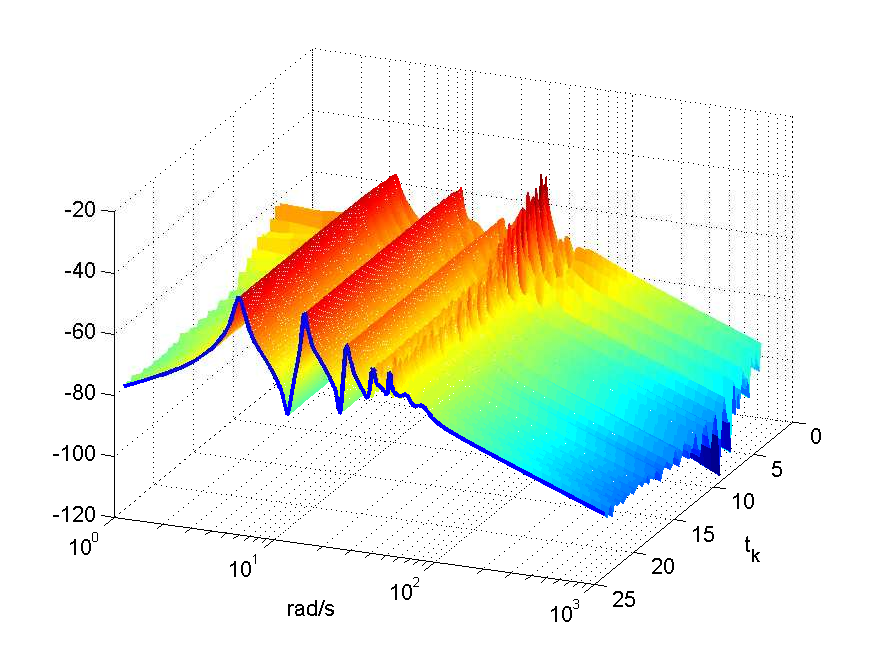
\includegraphics[width=0.8\columnwidth]{imgs/buildmagnitude.pdf}
\caption[Short description for list of figures]{This figure is taken from \cite{Sca:16}.}
\label{fig-magnitude}
\end{figure}%




\section{How to define Tables?}


In this section tables, equation etc examples are given. As given in Table~\ref{tab:1}, xxxxxxxxxx can be.

\begin{table*}[htbp]
	\caption{Comparison of Various Methods.}
	\begin{center}
		\begin{tabular}{l l l l l l l}
			%\hline
			%\multicolumn{7}{c}{Computation Times(in ms) for controllers} \\
			\cline{1-7}
			%Systems&&  IP System\\
			\hline
             Methods &  & Method 1&  &  & Method 2& \\
			\cline{1-7}
			Operations $\setminus$ Cases & Case 1& Case 2& Case 3 & Case 1 & Case 2 & Case 3\\
			\hline
			Operation 1 & 0.93684	&0.89219	&1.5028	&1.2275 &2.6182	&1.1922\\
            Operation 2 & 0.053503	&0.061289	&0.049883	&0.038601 &0.045261	&0.039763\\
            Operation 3 & 0.20027	&0.63789	&0.20335	&0.19014 &1.6918	&0.19196\\
            Operation 4 &0.28225	&0.40756	&0.32971	&0.24073 &0.3323	&0.2559\\
            Operation Final &1.4729	&1.9989	&2.0857  &1.6969 &4.6875	&1.6798\\
			\hline
		\end{tabular}
	\end{center}
	% \caption{Computation Times(in ms) for controllers}
	\label{tab:1}
\end{table*}
%
%



\section{How to define Algorithms and depict Flowcharts?}
An example for a pseudo code is given below. In order to cite an algorithm don't forget to label your algorithms such as "$\text{\label{alg:1}}$" . Algorithm~\ref{alg:1} is given below :
\begin{algorithm}
\caption{An algorithm with caption}\label{alg:1}
\begin{algorithmic}
\Require $n \geq 0$
\Ensure $y = x^n$
\State $y \gets 1$
\State $X \gets x$
\State $N \gets n$
\While{$N \neq 0$}
\If{$N$ is even}
    \State $X \gets X \times X$
    \State $N \gets \frac{N}{2}$  \Comment{This is a comment}
\ElsIf{$N$ is odd}
    \State $y \gets y \times X$
    \State $N \gets N - 1$
\EndIf
\EndWhile
\end{algorithmic}
\end{algorithm}

You can reach comprehensive information about Alogirthms etc via \url{https://www.overleaf.com/learn/latex/Algorithms}

Flow chart detailed informations are here \url{https://www.overleaf.com/learn/latex/LaTeX_Graphics_using_TikZ%3A_A_Tutorial_for_Beginners_(Part_3)%E2%80%94Creating_Flowcharts}



\tikzstyle{startstop} = [rectangle, rounded corners, 
minimum width=3cm, 
minimum height=1cm,
text centered, 
draw=black, 
fill=red!30]

\tikzstyle{io} = [trapezium, 
trapezium stretches=true, % A later addition
trapezium left angle=70, 
trapezium right angle=110, 
minimum width=3cm, 
minimum height=1cm, text centered, 
draw=black, fill=blue!30]

\tikzstyle{process} = [rectangle, 
minimum width=3cm, 
minimum height=1cm, 
text centered, 
text width=3cm, 
draw=black, 
fill=orange!30]

\tikzstyle{decision} = [diamond, 
minimum width=3cm, 
minimum height=1cm, 
text centered, 
draw=black, 
fill=green!30]
\tikzstyle{arrow} = [thick,->,>=stealth]


 \begin{tikzpicture}
        \node (start) [startstop] {Start};
        \node (input) [process, below of=start, yshift=-1.5cm] {Enter exam score};
        \node (decision) [decision, below of=input, yshift=-2cm] {Score >= 50?};
        \node (pass) [process, right of=decision, xshift=4cm] {Pass};
        \node (fail) [process, below of=decision, yshift=-2cm] {Fail};
        \node (end) [startstop, below of=fail, yshift=-1.5cm] {End};
        
        \draw [arrow] (start) -- (input);
        \draw [arrow] (input) -- (decision);
        \draw [arrow] (decision.east) -- node[anchor=south] {Yes} (pass.west);
        \draw [arrow] (pass.south) |- (end.east);
        \draw [arrow] (decision.south) -- node[anchor=east] {No} (fail.north);
        \draw [arrow] (fail.south) -- (end.north);
        
\end{tikzpicture}
    
\section{How to add ..... in Text?}
\subsection{How to add footnotes?}

Start writing your suggestions section here.\footnote{This is an example of footnote usage!}

\subsection{How to add Mathematical Expression in TEXT?}
You can add mathematical expression in text by definig expression inside two "\$". An axmple can be considered as $\sum_{i=1}^{\infty}\frac{1}{5}\frac{a+e^{-\lambda}}{2-\gamma_{\omega}}$


\subsection{How to add Abbreviations/Ancroynms in TEXT?}
You can use some acronyms: \ac{CAE}, \ac{EEE},\ac{ITU}, \ac{IEEE}, \ac{IFAC}, \ac{TOK}, \ac{PID} and \ac{LTI} systems in your text. The acronyms you have previously defined will appear in the list of acronyms as you mention them in the text.


\subsection{How to cite references in TEXT?}
Example of citation are here
\cite{AdaAroKre:71,PadScaAst:16a,PadScaAst:16b,PavVdWNij:06,PurBorVar:96,SLICOT,Sca:16,Sca:16a,Sca:16b,Sca:17,Sca:18}.
\subsection{How to refer equations, Tables, Figures, Algorithms etc in TEXT?}
adadada
% You can change the title of the conclusions by changing the text between { }
%\conclusions{Conclusions and future directions} % Do not remove - required

\EthicalRulesComplianceStatement{Ethical Rules Compliance Statement} % If you need a label for this chapter

\IndividualContributionStatement{Individual Contribution Statement}


\MultiobjectivecriteriaEngineeringStandards{Constraints and Engineering Standards Used in the Report} % If you need a label for this chapter




% EDIT THE CONTENT OF THE FILE
% Conclusions.tex
% You can find it under the folder 
% "chapters" on the left column

% APPENDICES ARE OPTIONAL
% COMMENT OUT BOTH LINES BELOW TO REMOVE THEM
% ADD CHAPTERS TO ADD MULTIPLE APPENDICES
\appendix 
\doublespacing % Do not change - required

\chapter{TIA Portal Program}

\thesisspacing % Do not change - required

In Chapter4, it was stated that a program was written in the TIA Portal software on PLCSim in order for the simulation environment created in the Factory IO environment to work correctly.
Here, the program written in the TIA Portal will be examined. As seen in Figures A1 and A2 below, the program consists of a total of 7 function blocks. Function blocks were preferred because the program does not look too complicated and is easier to examine and write.
\begin{figure}[H]
    \centering
    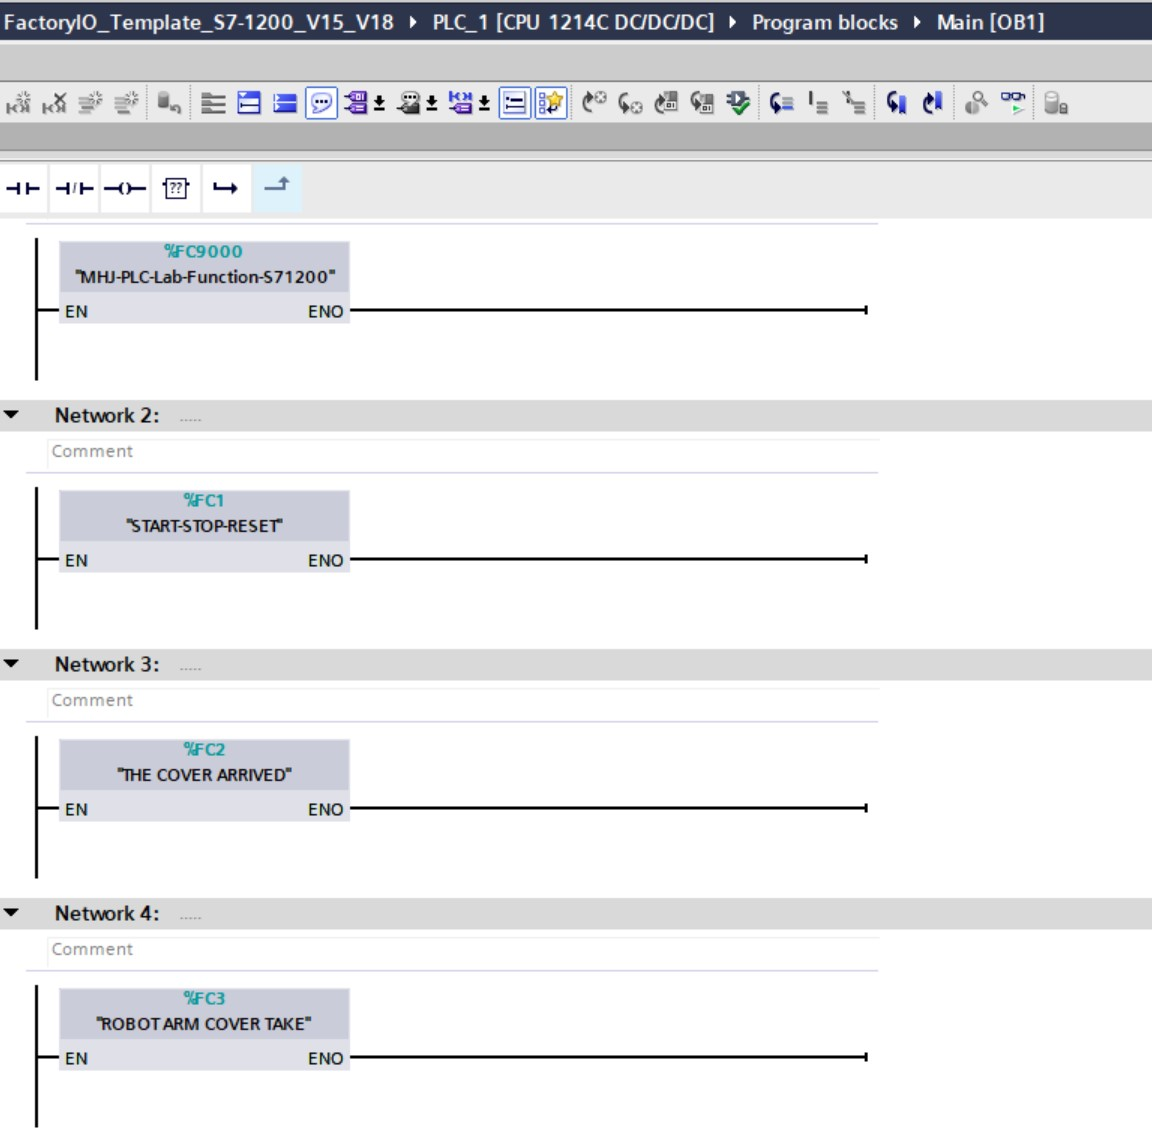
\includegraphics[width=0.70\columnwidth]{imgs/io/tia1.jpg}
    \caption[First four lines of the program]{First four lines of the program}
    \label{fig-magnitude}
\end{figure}%    
    \begin{figure}[H]
        \centering
        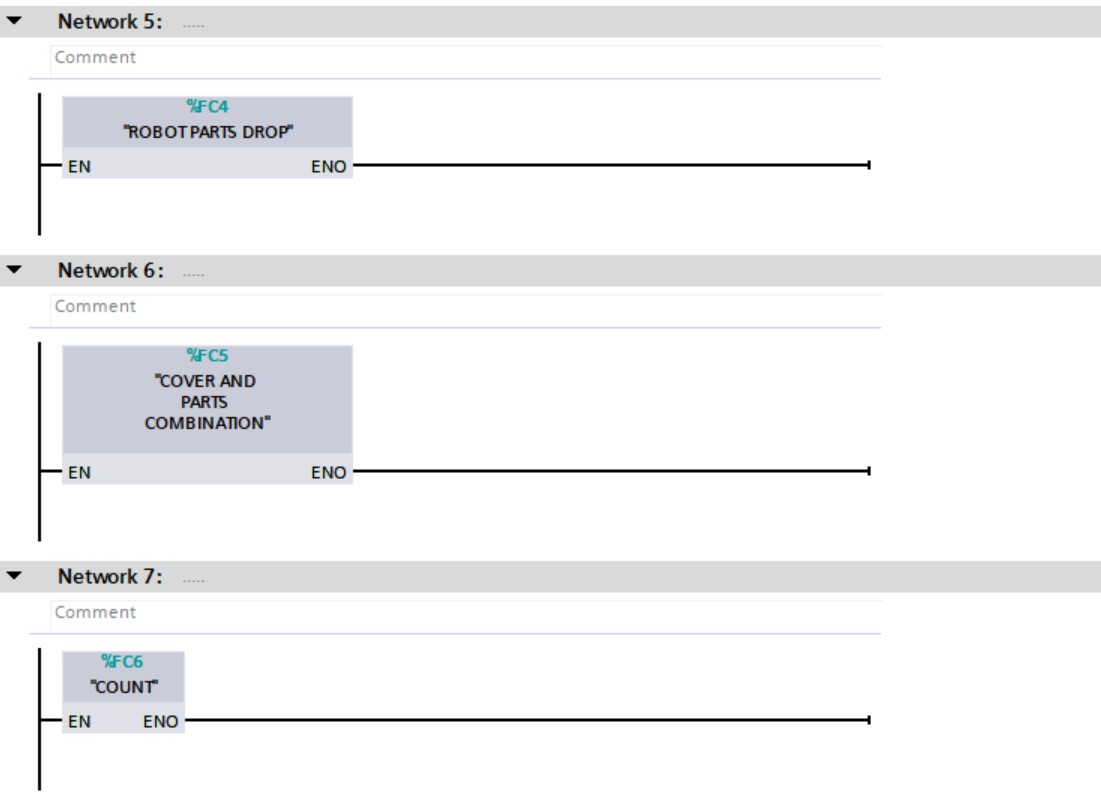
\includegraphics[width=0.70\columnwidth]{imgs/io/tia2.jpg}
        \caption[Last 3 lines of the program]{Last 3 lines of the program}
        \label{fig-magnitude}
    \end{figure}%
    Here, the first function block contains a ready-made function to establish the connection between TIA Portal and Factory IO. The internal structure of the block can be seen below.
\begin{figure}
    \centering
    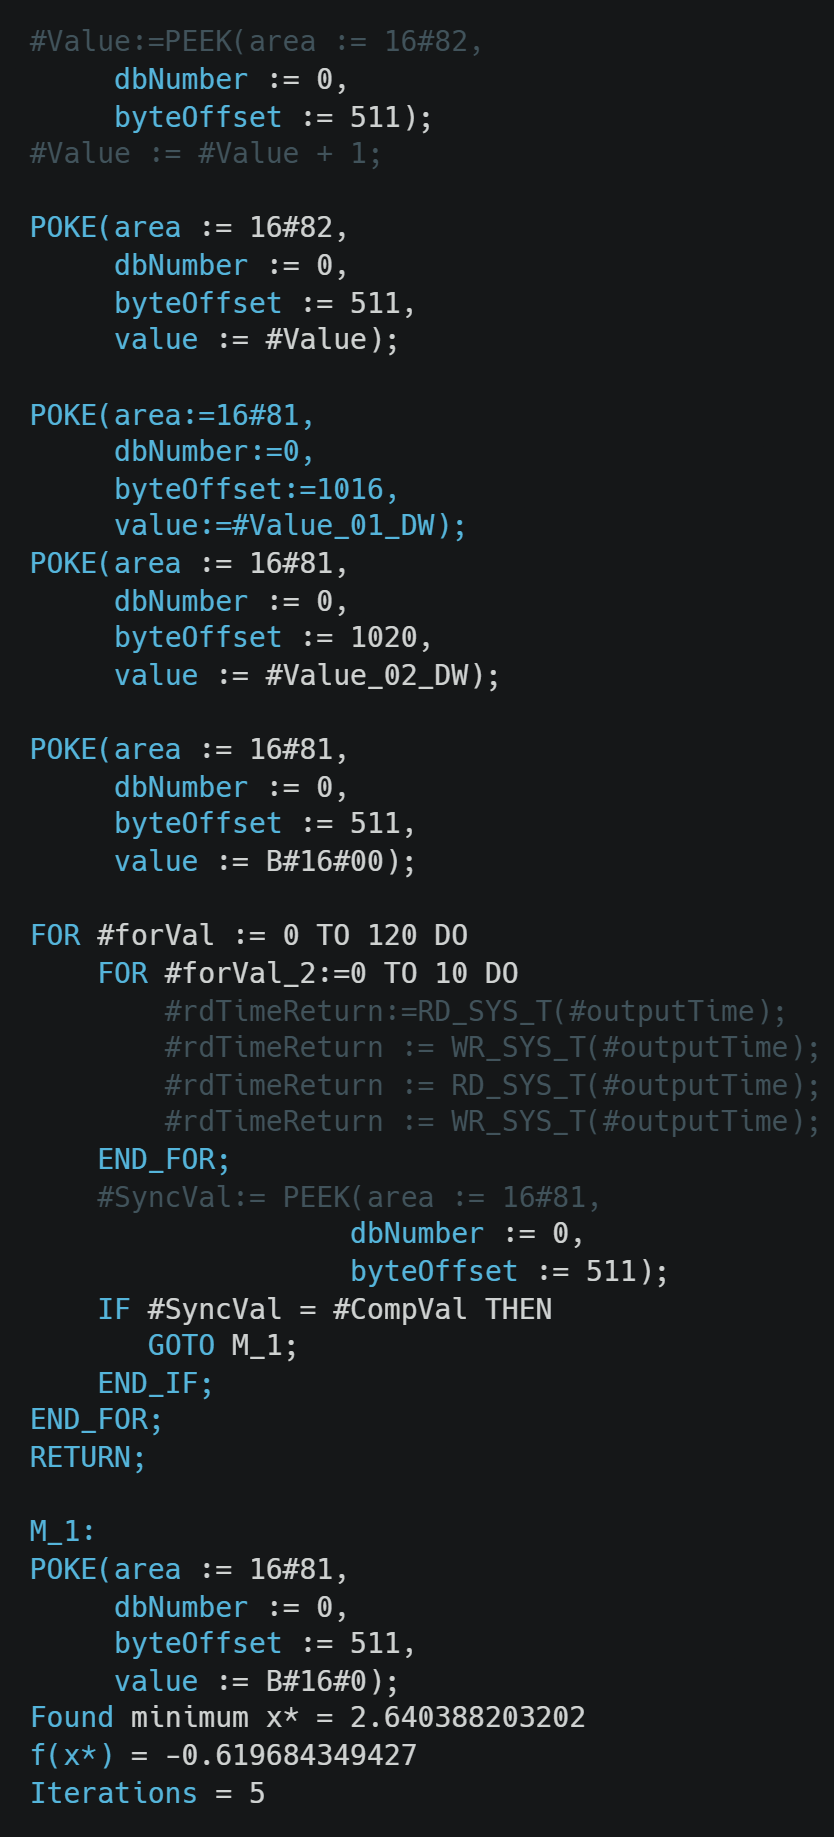
\includegraphics[width=0.50\columnwidth]{imgs/io/carbon.png}
    \caption[Function block 0]{Function block 0}
    \label{fig-magnitude}
\end{figure}%   

The function block seen in Figure A.4 above aims to start the system. Since the emergency stop button is normally connected to a closed contact in Factory IO, an open contact is connected here. Then, when the start button is pressed, the system starts.
\begin{figure}
    \centering
    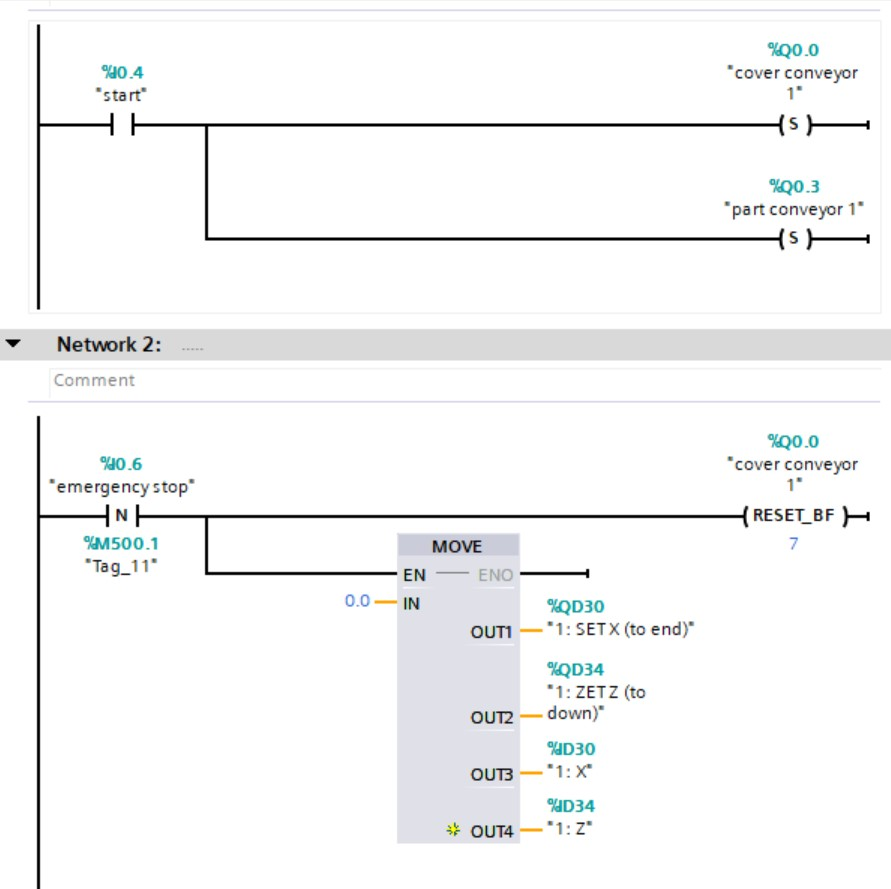
\includegraphics[width=0.60\columnwidth]{imgs/io/tia3.jpg}
    \caption[Function block 1]{Function block 1}
    \label{fig-magnitude}
\end{figure}%   


\begin{figure}[H]
    \centering
    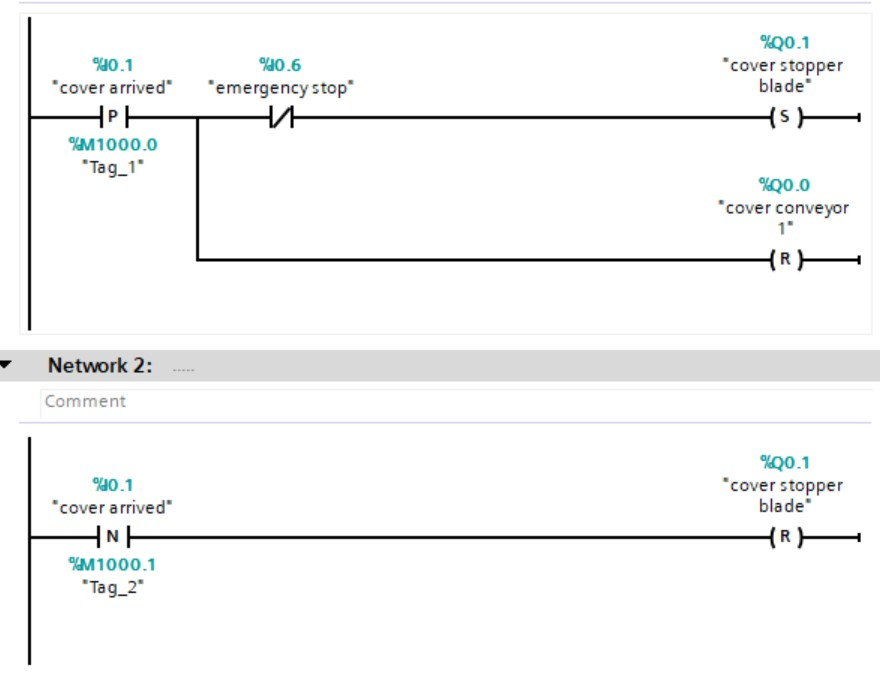
\includegraphics[width=0.60\columnwidth]{imgs/io/tia4.jpg}
    \caption[Function block 2]{Function block 2}
    \label{fig-magnitude}
\end{figure}% 
As seen in Figure A.5 above, when the sensor detecting the cover conveyor is active, the blade on the relevant side closes and the conveyor it comes to stops. When the sensor stops detecting, the blade opens again.

\begin{figure}[h!]
    \centering
    \begin{minipage}{0.45\textwidth}  
        \centering
        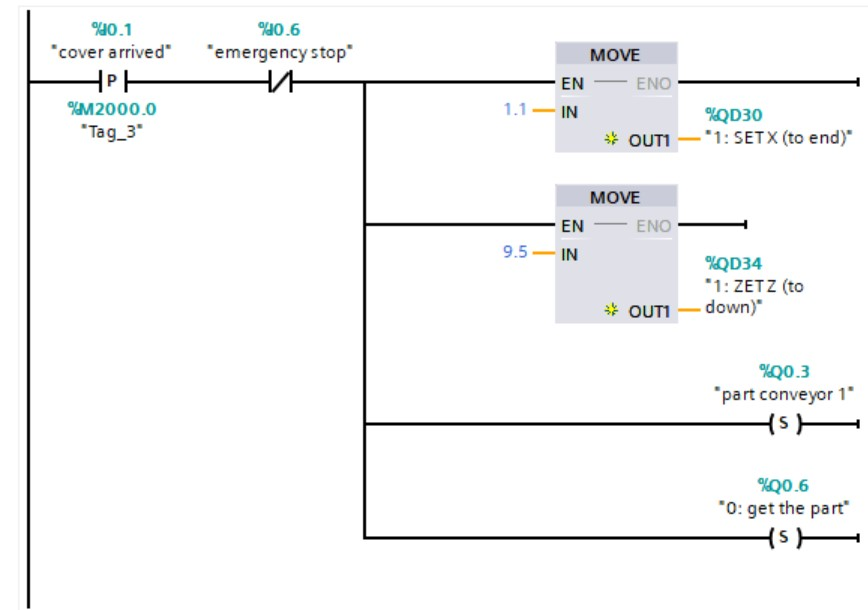
\includegraphics[width=\textwidth]{imgs/io/tia5.1.jpg}  
        \caption[Function blok 3 Network1]{Function blok 3 Network1}
        \label{fig:first}
    \end{minipage} \hfill  
    \begin{minipage}{0.45\textwidth}  
        \centering
        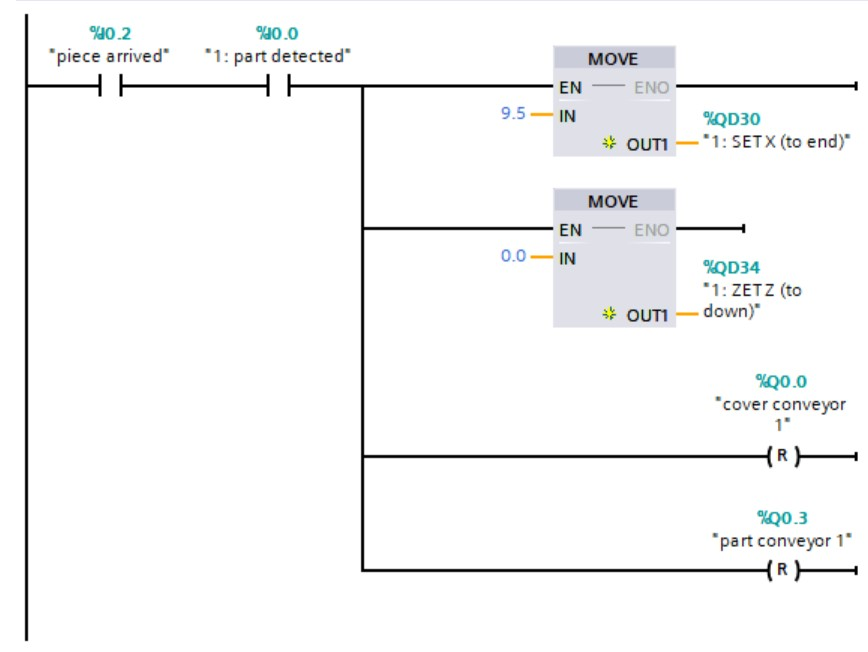
\includegraphics[width=\textwidth]{imgs/io/tia5.2.jpg}  
        \caption[Function blok 3 Network2]{Function blok 3 Network2}
        \label{fig:second}
    \end{minipage}
\end{figure}

In Figure A.6 above, after the lid is detected, the robot arm is provided with the help of a gripper to take the lid. These values ​​are provided to the x and z coordinates that were previously set by trial, that is, to be approximately on top of the lid.
In Figure A.7, the lid is taken to the determined coordinates and made ready to be combined with the part.

\begin{figure}[H]
    \centering
    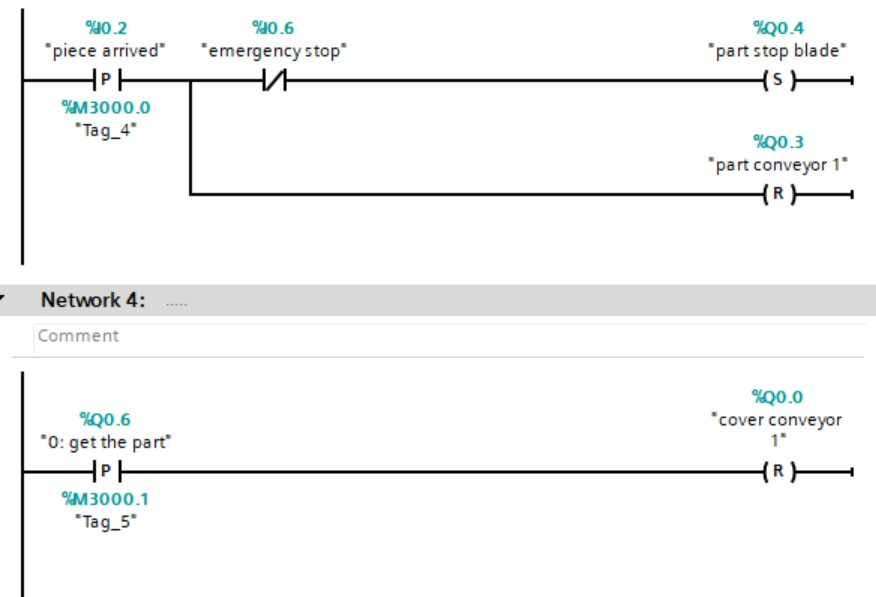
\includegraphics[width=0.60\columnwidth]{imgs/io/tia5.3.jpg}
    \caption[Function block 3 Network3 and Network4]{Function block 3 Network3 and Network4}
    \label{fig-magnitude}
\end{figure}% 

In Figure A.8 above, when the part sensor detects the object, the blade becomes active and the conveyor on which it stands goes into the off position. At the same time, after the gripper holds the lid, the lid conveyor stops accordingly.

\begin{figure}[H]
    \centering
    \begin{minipage}{0.45\textwidth}  
        \centering
        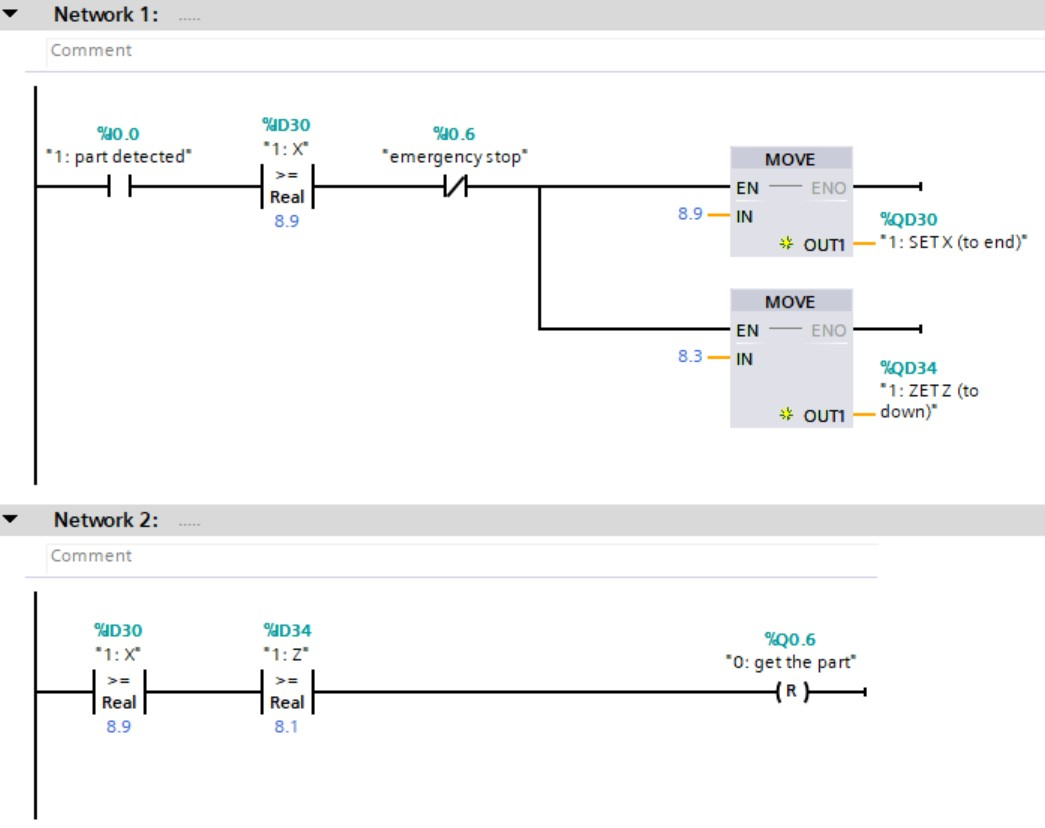
\includegraphics[width=\textwidth]{imgs/io/tia6.1.jpg}  
        \caption[Function blok 4 Network1 and Network2]{Function blok 4 Network1 and Network2}
        \label{fig:first}
    \end{minipage} \hfill  
    \begin{minipage}{0.45\textwidth}  
        \centering
        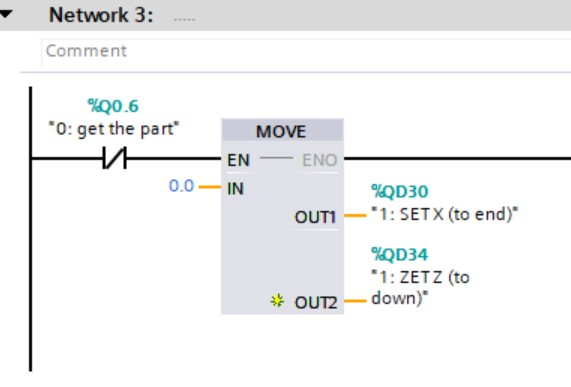
\includegraphics[width=\textwidth]{imgs/io/tia6.2.jpg} 
        \caption[Function blok 4 Network3]{Function blok 4 Network3}
        \label{fig:second}
    \end{minipage}
\end{figure}

In Figure A.9 above, when the robot arm reaches the desired position, it is assembled by dropping the cover onto the part.

In Figure A.10, the robot arm returns to the set starting position after releasing the lid.

\begin{figure}[H]
    \centering
    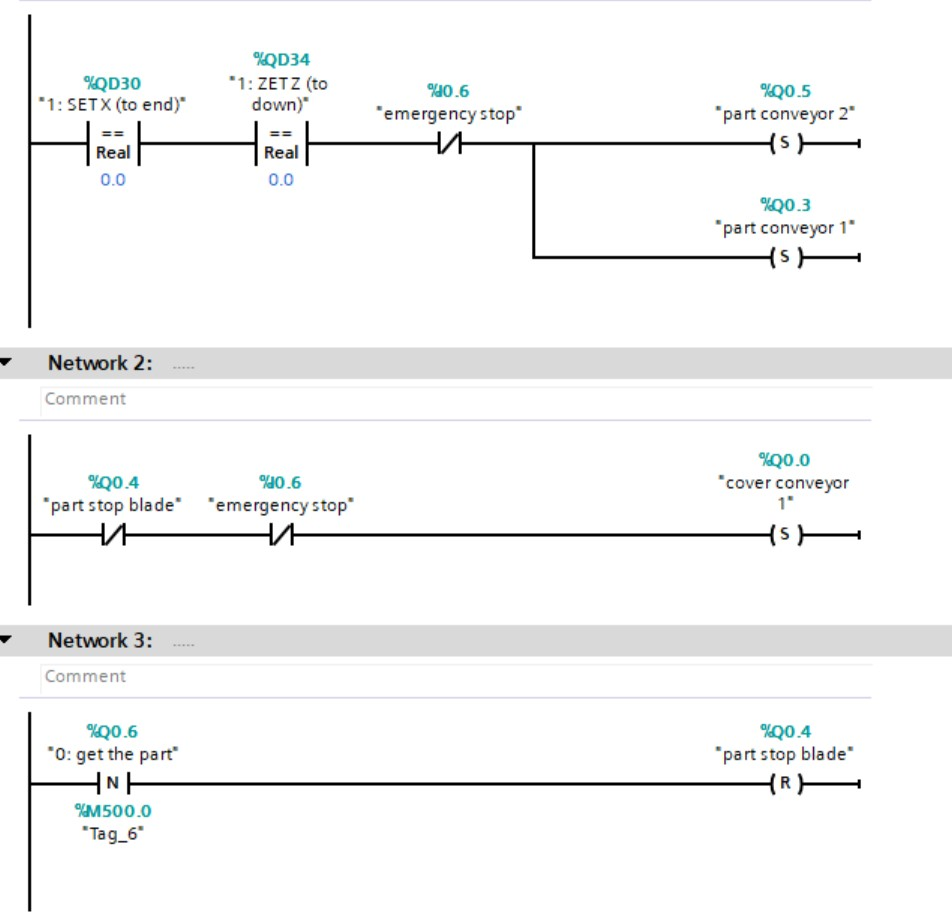
\includegraphics[width=0.60\columnwidth]{imgs/io/tia7.1.jpg}
    \caption[Function block 5 Network1 to Network3]{Function block 5 Network1 to Network3}
    \label{fig-magnitude}
\end{figure}% 

In Network 1 and Network 2 above, the conveyors are restarted. In Network 3, after the gripper releases the cover, the blade in front of the product is lifted. In this way, the product can move forward on the part conveyor.

\begin{figure}[H]
    \centering
    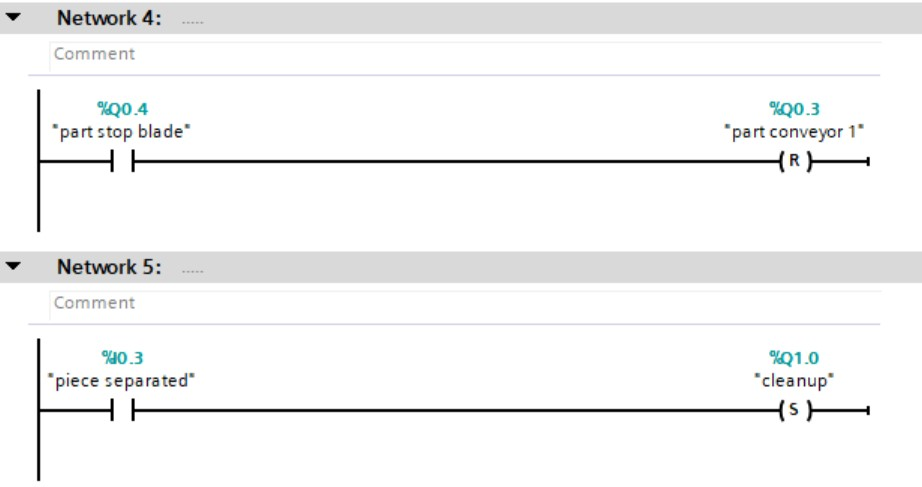
\includegraphics[width=0.60\columnwidth]{imgs/io/tia7.2.jpg}
    \caption[Function block 5 Network4 and Network5]{Function block 5 Network4 and Network5}
    \label{fig-magnitude}
\end{figure}% 

In Network 4 above, if the part blade is open, unnecessary operation of the 1st part conveyor is prevented. In this way, energy saving is achieved. In Network 5, after the created part passes the part separation sensor, the remover that cleans the created part at the end of the belt is activated.

\begin{figure}[H]
    \centering
    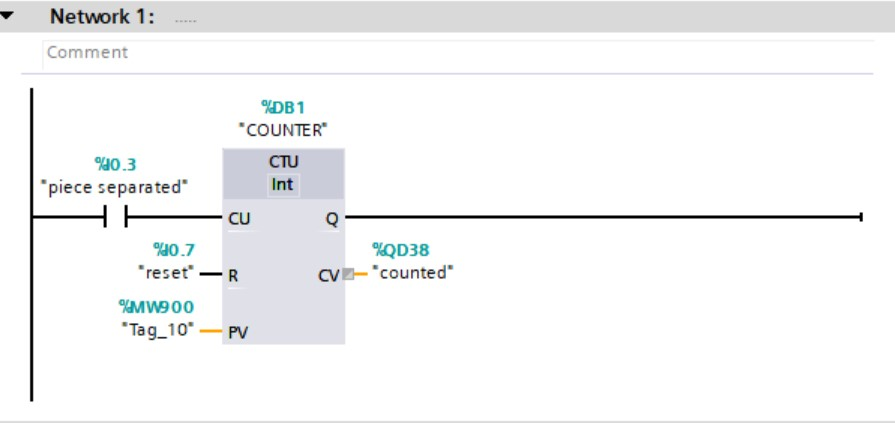
\includegraphics[width=0.60\columnwidth]{imgs/io/tia8.jpg}
    \caption[Function block 6]{Function block 6}
    \label{fig-magnitude}
\end{figure}% 
Here, a program part is seen where the products produced in the system are counted with an up counter block after the object created passes through the part separation sensor. A reset button is assigned to reset the counting process.


\doublespacing % Do not change - required

\chapter{DC Motor Matlab Modeling}

\thesisspacing % Do not change - required

Below you can see the modeling of a DC motor in the Simulink program and the internal structure of the DC motor.

\begin{figure}[H]
    \centering
    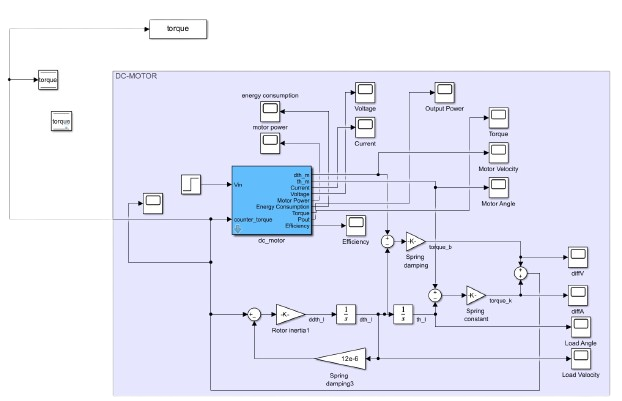
\includegraphics[width=0.9\columnwidth]{imgs/io/dc1.png}
    \caption[Simulink model of the DC motor]{Simulink model of the DC motor}
    \label{fig-magnitude}
\end{figure}%

A Simulink drawing of a DC model was created above. From here, the current, torque, etc. quantities were taken and the energy consumption and efficiency of the motor were measured.

\begin{figure}[h]
        \centering
        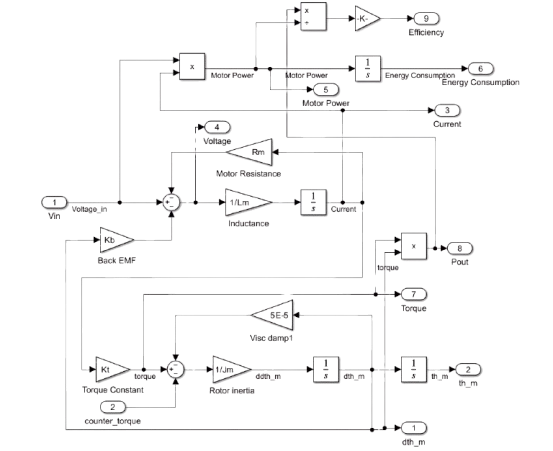
\includegraphics[width=0.9\columnwidth]{imgs/io/dc2.png}
        \caption[Inside of the DC motor]{Inside of the DC motor}
        \label{fig-magnitude}
\end{figure}%

The internal structure of a DC motor is shown above. Depending on these, any information desired from the current-time expression of the system to the efficiency expression can be obtained.

The current is equal to the integral of the output voltage divided by the inductance value with
respect to time. The current-time graph is shown below:


\begin{equation}
i = \int_{0}^{t} \frac{V_{\text{out}}}{L_m} \, dt 
\end{equation}



\begin{figure}[H]
    \centering
    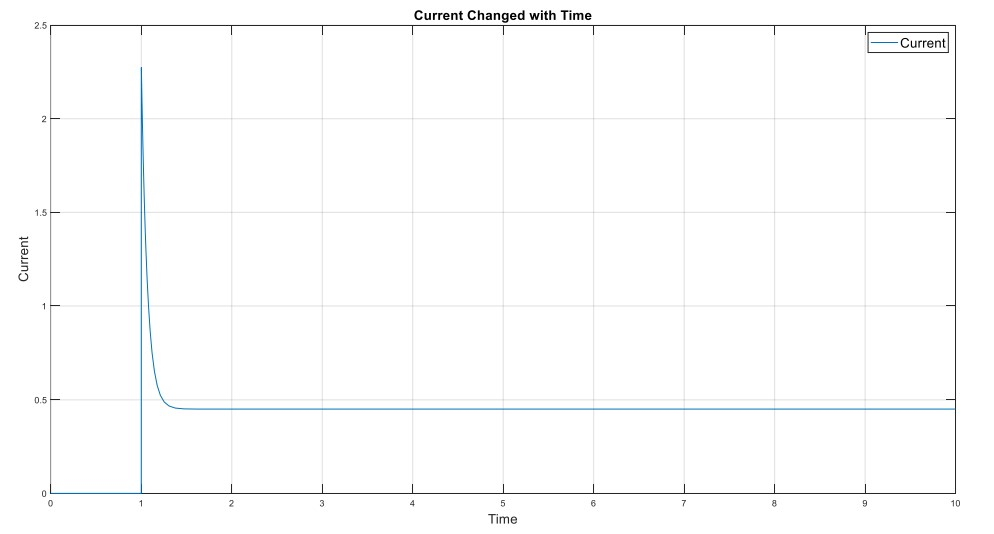
\includegraphics[width=0.7\columnwidth]{imgs/io/a.jpg}
    \caption[Current-time graph]{Current-time graph}
    \label{fig-magnitude}
\end{figure}%

Torque is equal to the product of the torque constant and the current. Below is the torque time
graph.

\begin{equation}
u = K_t i
\end{equation}

\begin{figure}[H]
    \centering
    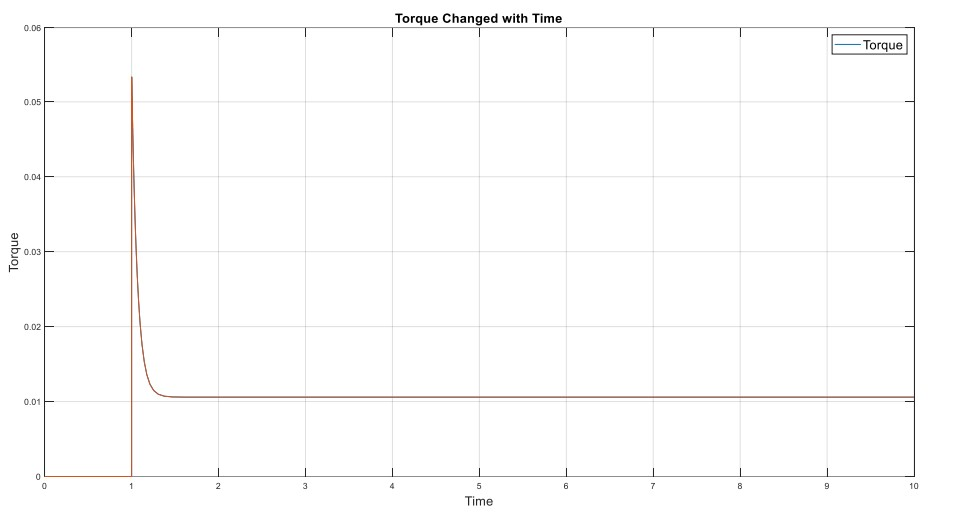
\includegraphics[width=0.7\columnwidth]{imgs/io/b.jpg}
    \caption[Torque-time graph]{Torque-time graph}
    \label{fig-magnitude}
\end{figure}%

The counter torque created by the load is as shown in the graph below. This acts as a
distorting effect on the DC motor.

\begin{figure}[H]
    \centering
    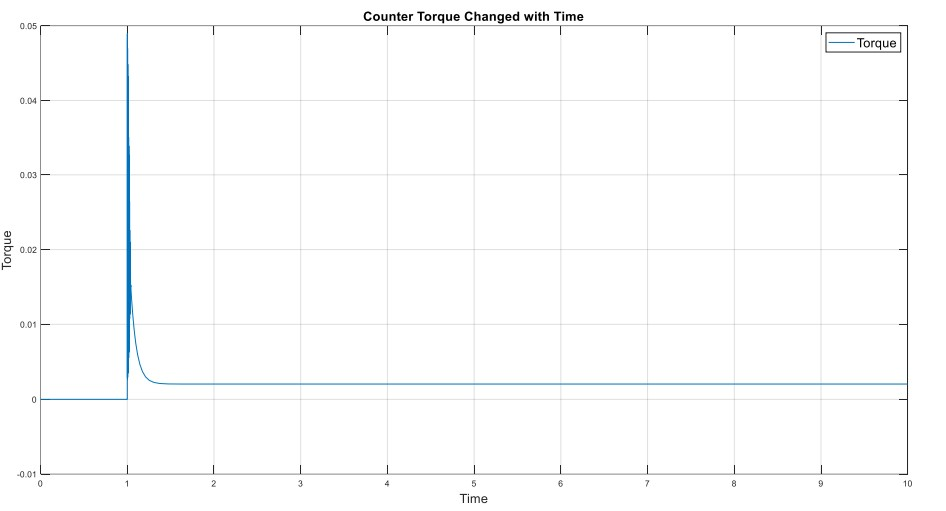
\includegraphics[width=0.7\columnwidth]{imgs/io/c.jpg}
    \caption[Counter torque-time graph]{Counter torque-time graph}
    \label{fig-magnitude}
\end{figure}%

The angular velocity of the motor is equal to the integral of the angular acceleration of the
motor. Here we see that the motor increases rapidly and then settles to a constant value.

\begin{equation}
w = \int_0^t \alpha \, dt    
\end{equation}

\begin{figure}[H]
    \centering
    \includegraphics[width=0.7\columnwidth]{imgs/io/d.jpg}
    \caption[Angular velocity-time graph]{Angular velocity-time graph}
    \label{fig-magnitude}
\end{figure}%

The angular position of the motor, that is, its angle, is equal to the integral of the angular velocity
of the motor. In other words, it is the second integral of its angular acceleration. Here, it is seen
that the angular increases linearly. Its unit is radian.

\begin{equation}
\theta = \int_{0}^{t} \int_{0}^{t} \alpha \, dt    
\end{equation}

\begin{figure}[H]
    \centering
    \includegraphics[width=0.7\columnwidth]{imgs/io/e.jpg}
    \caption[Motor angle-time graph]{Motor angle-time graph}
    \label{fig-magnitude}
\end{figure}%

The speed-time graph of the load is as follows
\begin{figure}[H]
    \centering
    \includegraphics[width=0.7\columnwidth]{imgs/io/f.jpg}
    \caption[load speed-time graph]{load speed-time graph}
    \label{fig-magnitude}
\end{figure}%

The angular position-time graph of the load is as follows.
\begin{figure}[H]
    \centering
    \includegraphics[width=0.7\columnwidth]{imgs/io/g.jpg}
    \caption[load angular position-time graph]{load angular position-time graph}
    \label{fig-magnitude}
\end{figure}%

In the simulation, the voltage of the DC motor was initially given as 5 with a step. Then, with
the effect of back emf, resistance and coil, this voltage was equalized to zero.

\begin{equation}
V = V_{in} - V_{backemf} - RI 
\end{equation}

\begin{figure}[H]
    \centering
    \includegraphics[width=0.7\columnwidth]{imgs/io/h.jpg}
    \caption[DC motor voltage-time graph]{DC motor voltage-time graph}
    \label{fig-magnitude}
\end{figure}%

Motor power is formulated as the product of input voltage and current. Motor power time graph
is as follows

\begin{equation}
P_{DC} = V_{in} I    
\end{equation}

\begin{figure}[H]
    \centering
    \includegraphics[width=0.7\columnwidth]{imgs/io/ı.jpg}
    \caption[Motor power-time graph]{Motor power-time graph}
    \label{fig-magnitude}
\end{figure}%

Output power is equal to the product of the system torque and the motor speed. It is an important
parameter in calculating efficiency. The graph is as follows.

\begin{equation}
P_{out} = \tau W
\end{equation}

\begin{figure}[H]
    \centering
    \includegraphics[width=0.7\columnwidth]{imgs/io/i.jpg}
    \caption[Output power-time graph]{Output power-time graph}
    \label{fig-magnitude}
\end{figure}%

In physics, the energy consumed is calculated as the integral of the power. Here, the integral of
the motor power represents the energy consumption of the system

\begin{equation}
Consumption = \int_0^t P_{out} \, dt 
\end{equation}

\begin{figure}[H]
    \centering
    \includegraphics[width=0.7\columnwidth]{imgs/io/j.jpg}
    \caption[Energy consumtion-time graph]{Energy consumtion-time graph}
    \label{fig-magnitude}
\end{figure}%

Efficiency is the measure of the extent to which the power given at the input of a system can be
preserved at the output. Because the integral of the power gives the speed. Here, efficiency is
the ratio of the output power to the input power. A gain block was multiplied to calculate as a
percentage. It was determined that our engine operated at 80% efficiency under these
parameters and this load.

\begin{equation}
\eta = \frac{P_{out}}{P_{DC}} 100    
\end{equation}

\begin{figure}[H]
    \centering
    \includegraphics[width=0.7\columnwidth]{imgs/io/k.jpg}
    \caption[Efficiency-time graph]{Efficiency-time graph}
    \label{fig-magnitude}
\end{figure}%





 % Example second appendix (need to create the file in "chapters")


\cleardoublepage % Do not change - required
\RemoveLabels % Do not change - required
\thesisspacing % Do not change - required
\printbibliography[title={References},heading=bibintoc] % Do not change - required

%=============    CV/Resume Section ==================
%You can add as many CVs as the number of students. Comment the CVs that will not be used with the "%" sign like "%\ResumeTwo{Resume2}% If you need a label for this chapter." 


\ResumeOne{Resume 1} % Add Resume of the 1st author
\ResumeTwo{Resume 2} % Add Resume of the 2nd author if needed
\ResumeThree{Resume 3} % Add Resume of the 3rd author if needed


%permission might be required for teams with more than 5 students
%\ResumeSix{Resume 6} % Add Resume of the 6th author if needed 
%\ResumeSeven{Resume 7} % Add Resume of the 7th author if needed



%\doublespacing % Do not change - required

\chapter{How To ...... in\LaTeX ?}
\label{chHT}

%%%%%%%%%%%%%%%%%%%%%%%%%%%%%%%%%%%%%%%
% IMPORTANT
\begin{spacing}{1} %THESE FOUR
\minitoc % LINES MUST APPEAR IN
\end{spacing} % EVERY
\thesisspacing % CHAPTER
% COPY THEM IN ANY NEW CHAPTER
%%%%%%%%%%%%%%%%%%%%%%%%%%%%%%%%%%%%%%%

{\color{red}This section provides detailed examples of equations, tables, figures, etc. that you will use in LATEX to help you with your interim and final reports. Please review the recommended websites!!!!!!!}

\section{Introduction}

In this section, some crucial point about how to fill this template are given such as formulation, figures, tables etc.

\section{How to define an equation ?}
\medskip
A simple and a complex examples are given in equation (\ref{eq:simpleexample}) and equation (\ref{eq:complexexample})

\begin{equation}
    u(t) = K_p e \left( t\right) + K_i \int_0^t \left( \tau\right) dt + K_d \frac{d e \left( t\right)}{dt}
    \label{eq:simpleexample}
\end{equation}

%
%
\begin{equation}
\begin{split}
& \mathbf{F_1}=\{i \ | \ |\beta_i|=Z, |G\left(\mathbf{x_i}\right)|\geq \epsilon \} \\
& \mathbf{F_2}=\{i \ | \ 0< |\alpha_i|<P, |G_2\left(\mathbf{x_{ijkl}}\right)|=0  \} \\ 
& \mathbf{\omega_{PSA}}=\{k \ | \ |\lambda_i|=0, | \phi\left(\mathbf{x_i}\right)|\leq \varepsilon  \}
\end{split}
\label{eq:complexexample}
\end{equation}
%
%
For more detailed informations, you can use \url{https://www.overleaf.com/learn/latex/Mathematical_expressions} and "Further reading" sections given in previous website.
%
%
\subsection{How to define matrix?}


\begin{equation}
\boldsymbol{\Omega}=\begin{bmatrix}
	\Omega_{s_0}\\
	\Omega_{s_1}\\
	\vdots\\
	\Omega_{s_k}
	\end{bmatrix} =-\mathbf{\Theta}\begin{bmatrix}
	1\\
	2\\
	\vdots\\
	K
	\end{bmatrix} \ , \
	\label{eq:10}
\end{equation}


\begin{equation}
%\begin{split}
\boldsymbol{\Omega}=\begin{bmatrix}
	\Omega_{s_0}\\
	\Omega_{s_1}\\
	\vdots\\
	\Omega_{s_k}
	\end{bmatrix} =-\mathbf{\theta}\begin{bmatrix}
	1\\
	2\\
	\vdots\\
	K
	\end{bmatrix} \ , \
    	\mathbf{\theta}=\begin{bmatrix}
	\theta_{11} & \theta_{12} & \cdots &\theta_{1k} \\
	\theta_{21} & \theta_{22} & \cdots &\theta_{2k} \\
	\vdots & \vdots & \ddots & \vdots \\
    \theta_{k1} & \theta_{k2} & \cdots &\theta_{kk}
	\end{bmatrix}^{-1}
%\end{split}        
	\label{eq:10}
\end{equation}
%
%






\subsection{How to split Long equations?}

You can use "split" command given as below:

\begin{equation}
\begin{split}
&\boldsymbol{\Omega}=\begin{bmatrix}
	\Omega_{s_0}\\
	\Omega_{s_1}\\
	\vdots\\
	\Omega_{s_k}
	\end{bmatrix} =-\mathbf{\theta}\begin{bmatrix}
	1\\
	2\\
	\vdots\\
	K
	\end{bmatrix} \ , \\
    &
    	\mathbf{\theta}=\begin{bmatrix}
	\theta_{11} & \theta_{12} & \cdots &\theta_{1k} \\
	\theta_{21} & \theta_{22} & \cdots &\theta_{2k} \\
	\vdots & \vdots & \ddots & \vdots \\
    \theta_{k1} & \theta_{k2} & \cdots &\theta_{kk}
	\end{bmatrix}^{-1}
\end{split}        
	\label{eq:10}
\end{equation}

%
%
For detailed information you can use the following website.

\medskip
For detailed information you can use the following website.\\
\url{https://www.overleaf.com/learn/latex/Aligning_equations_with_amsmath}


\subsection{Significant Greek Symbols utilized in \LaTeX}

Some symbols are given below



In addition to these, you can find much more detailed information on the website below. In addition, LLM structures will be very helpful.

\begin{itemize}
\item \url{https://www.overleaf.com/learn/latex/List_of_Greek_letters_and_math_symbols}
\item \url{https://ftp.cc.uoc.gr/mirrors/CTAN/info/symbols/comprehensive/symbols-a4.pdf}
\item \url{https://www.geeksforgeeks.org/greek-alphabet-symbols/}

\item Your LLM Friends(ChatGPT, Deepseek etc) 
\end{itemize}


\subsubsection{Greek Alphabet}
\subsubsection{Lowercase Letters}
\begin{tabular}{ll | ll | ll}
\textbackslash alpha & $\alpha$ & \textbackslash nu & $\nu$ & \textbackslash upsilon & $\upsilon$ \\
\textbackslash beta & $\beta$ & \textbackslash xi & $\xi$ & \textbackslash phi & $\phi$ \\
\textbackslash gamma & $\gamma$ & \textbackslash omicron & $o$ & \textbackslash chi & $\chi$ \\
\textbackslash delta & $\delta$ & \textbackslash pi & $\pi$ & \textbackslash psi & $\psi$ \\
\textbackslash epsilon & $\epsilon$ & \textbackslash rho & $\rho$ & \textbackslash omega & $\omega$ \\
\textbackslash zeta & $\zeta$ & \textbackslash sigma & $\sigma$ &  &  \\
\textbackslash eta & $\eta$ & \textbackslash tau & $\tau$ &  &  \\
\textbackslash theta & $\theta$ & \textbackslash iota & $\iota$ &  &  \\
\end{tabular}

\subsubsection{Uppercase Letters}
\begin{tabular}{ll | ll | ll}
\textbackslash Gamma & $\Gamma$ & \textbackslash Lambda & $\Lambda$ & \textbackslash Sigma & $\Sigma$ \\
\textbackslash Delta & $\Delta$ & \textbackslash Xi & $\Xi$ & \textbackslash Upsilon & $\Upsilon$ \\
\textbackslash Theta & $\Theta$ & \textbackslash Pi & $\Pi$ & \textbackslash Phi & $\Phi$ \\
\textbackslash Omega & $\Omega$ & \textbackslash Psi & $\Psi$ &  &  \\
\end{tabular}

\subsubsection{Mathematical Symbols}
\subsubsection{Commonly Used Symbols}
\begin{tabular}{ll | ll | ll}
\textbackslash infty & $\infty$ & \textbackslash pm & $\pm$ & \textbackslash times & $\times$ \\
\textbackslash sum & $\sum$ & \textbackslash prod & $\prod$ & \textbackslash int & $\int$ \\
\textbackslash sqrt & $\sqrt{x}$ & \textbackslash frac & $\frac{a}{b}$ & \textbackslash lim & $\lim$ \\
\textbackslash sin & $\sin x$ & \textbackslash cos & $\cos x$ & \textbackslash tan & $\tan x$ \\
\textbackslash log & $\log x$ & \textbackslash exp & $\exp x$ & \textbackslash ln & $\ln x$ \\
\end{tabular}

\subsubsection{Relational Symbols}
\begin{tabular}{ll | ll | ll}
\textbackslash leq & $\leq$ & \textbackslash geq & $\geq$ & \textbackslash neq & $\neq$ \\
\textbackslash approx & $\approx$ & \textbackslash equiv & $\equiv$ & \textbackslash subset & $\subset$ \\
\textbackslash supset & $\supset$ & \textbackslash subseteq & $\subseteq$ & \textbackslash supseteq & $\supseteq$ \\
\end{tabular}

\subsubsection{Logic and Set Notation}
\begin{tabular}{ll | ll | ll}
\textbackslash forall & $\forall$ & \textbackslash exists & $\exists$ & \textbackslash neg & $\neg$ \\
\textbackslash in & $\in$ & \textbackslash notin & $\notin$ & \textbackslash emptyset & $\emptyset$ \\
\textbackslash cap & $\cap$ & \textbackslash cup & $\cup$ & \textbackslash subseteq & $\subseteq$ \\
\textbackslash wedge & $\wedge$ & \textbackslash vee & $\vee$ & \textbackslash Rightarrow & $\Rightarrow$ \\
\textbackslash Leftrightarrow & $\Leftrightarrow$ & \textbackslash bot & $\bot$ & \textbackslash top & $\top$ \\
\end{tabular}

\subsubsection{Brackets and Parentheses in Mathematical Expressions}
The following web site will help you for detailed information about Brackets and Parentheses " 
\url{https://www.overleaf.com/learn/latex/Brackets_and_Parentheses} " .




















\section{How to upload Figure etc?}


\begin{figure}
\centering
\includegraphics[width=0.8\columnwidth]{imgs/buildmagnitude.pdf}
\caption[Short description for list of figures]{This figure is taken from \cite{Sca:16}.}
\label{fig-magnitude}
\end{figure}%




\section{How to define Tables?}


In this section tables, equation etc examples are given. As given in Table~\ref{tab:1}, xxxxxxxxxx can be.

\begin{table*}[htbp]
	\caption{Comparison of Various Methods.}
	\begin{center}
		\begin{tabular}{l l l l l l l}
			%\hline
			%\multicolumn{7}{c}{Computation Times(in ms) for controllers} \\
			\cline{1-7}
			%Systems&&  IP System\\
			\hline
             Methods &  & Method 1&  &  & Method 2& \\
			\cline{1-7}
			Operations $\setminus$ Cases & Case 1& Case 2& Case 3 & Case 1 & Case 2 & Case 3\\
			\hline
			Operation 1 & 0.93684	&0.89219	&1.5028	&1.2275 &2.6182	&1.1922\\
            Operation 2 & 0.053503	&0.061289	&0.049883	&0.038601 &0.045261	&0.039763\\
            Operation 3 & 0.20027	&0.63789	&0.20335	&0.19014 &1.6918	&0.19196\\
            Operation 4 &0.28225	&0.40756	&0.32971	&0.24073 &0.3323	&0.2559\\
            Operation Final &1.4729	&1.9989	&2.0857  &1.6969 &4.6875	&1.6798\\
			\hline
		\end{tabular}
	\end{center}
	% \caption{Computation Times(in ms) for controllers}
	\label{tab:1}
\end{table*}
%
%



\section{How to define Algorithms and depict Flowcharts?}
An example for a pseudo code is given below. In order to cite an algorithm don't forget to label your algorithms such as "$\text{\label{alg:1}}$" . Algorithm~\ref{alg:1} is given below :
\begin{algorithm}
\caption{An algorithm with caption}\label{alg:1}
\begin{algorithmic}
\Require $n \geq 0$
\Ensure $y = x^n$
\State $y \gets 1$
\State $X \gets x$
\State $N \gets n$
\While{$N \neq 0$}
\If{$N$ is even}
    \State $X \gets X \times X$
    \State $N \gets \frac{N}{2}$  \Comment{This is a comment}
\ElsIf{$N$ is odd}
    \State $y \gets y \times X$
    \State $N \gets N - 1$
\EndIf
\EndWhile
\end{algorithmic}
\end{algorithm}

You can reach comprehensive information about Alogirthms etc via \url{https://www.overleaf.com/learn/latex/Algorithms}

Flow chart detailed informations are here \url{https://www.overleaf.com/learn/latex/LaTeX_Graphics_using_TikZ%3A_A_Tutorial_for_Beginners_(Part_3)%E2%80%94Creating_Flowcharts}



\tikzstyle{startstop} = [rectangle, rounded corners, 
minimum width=3cm, 
minimum height=1cm,
text centered, 
draw=black, 
fill=red!30]

\tikzstyle{io} = [trapezium, 
trapezium stretches=true, % A later addition
trapezium left angle=70, 
trapezium right angle=110, 
minimum width=3cm, 
minimum height=1cm, text centered, 
draw=black, fill=blue!30]

\tikzstyle{process} = [rectangle, 
minimum width=3cm, 
minimum height=1cm, 
text centered, 
text width=3cm, 
draw=black, 
fill=orange!30]

\tikzstyle{decision} = [diamond, 
minimum width=3cm, 
minimum height=1cm, 
text centered, 
draw=black, 
fill=green!30]
\tikzstyle{arrow} = [thick,->,>=stealth]


 \begin{tikzpicture}
        \node (start) [startstop] {Start};
        \node (input) [process, below of=start, yshift=-1.5cm] {Enter exam score};
        \node (decision) [decision, below of=input, yshift=-2cm] {Score >= 50?};
        \node (pass) [process, right of=decision, xshift=4cm] {Pass};
        \node (fail) [process, below of=decision, yshift=-2cm] {Fail};
        \node (end) [startstop, below of=fail, yshift=-1.5cm] {End};
        
        \draw [arrow] (start) -- (input);
        \draw [arrow] (input) -- (decision);
        \draw [arrow] (decision.east) -- node[anchor=south] {Yes} (pass.west);
        \draw [arrow] (pass.south) |- (end.east);
        \draw [arrow] (decision.south) -- node[anchor=east] {No} (fail.north);
        \draw [arrow] (fail.south) -- (end.north);
        
\end{tikzpicture}
    
\section{How to add ..... in Text?}
\subsection{How to add footnotes?}

Start writing your suggestions section here.\footnote{This is an example of footnote usage!}

\subsection{How to add Mathematical Expression in TEXT?}
You can add mathematical expression in text by definig expression inside two "\$". An axmple can be considered as $\sum_{i=1}^{\infty}\frac{1}{5}\frac{a+e^{-\lambda}}{2-\gamma_{\omega}}$


\subsection{How to add Abbreviations/Ancroynms in TEXT?}
You can use some acronyms: \ac{CAE}, \ac{EEE},\ac{ITU}, \ac{IEEE}, \ac{IFAC}, \ac{TOK}, \ac{PID} and \ac{LTI} systems in your text. The acronyms you have previously defined will appear in the list of acronyms as you mention them in the text.


\subsection{How to cite references in TEXT?}
Example of citation are here
\cite{AdaAroKre:71,PadScaAst:16a,PadScaAst:16b,PavVdWNij:06,PurBorVar:96,SLICOT,Sca:16,Sca:16a,Sca:16b,Sca:17,Sca:18}.
\subsection{How to refer equations, Tables, Figures, Algorithms etc in TEXT?}
adadada % Since this section is given for help in your thesis, don't forget to disable this section via \% sign before finalizing your report 



\end{document}
